\chapter{实数的连续性}

这一章我们首先介绍实数序列的极限概念, 然后研究了序列极限的基本性质, 最后证明了实数的连续性.

\section{实数序列的极限}

首先我们介绍实数序列的极限定义.

\section*{1. 实数序列的极限定义}

定义 从 $\mathbf{{N到R}}$ 的任一映射 $x : \mathbf{N} \rightarrow  \mathbf{R}$ 称为一个实数序列,简记为 $\left\langle  {x}_{n}\right\rangle$ . ${x}_{n}\left( {n \in  \mathbf{N}}\right)$ 称为此实数序列的第 $n$ 项或通项.

例1 设

1) ${x}_{n} = \frac{{a}^{n}}{n!}\left( {n \in  \mathbf{N}}\right)$ ,

2) ${x}_{n} = f\left( n\right) \left( {n \in  \mathbf{N}}\right)$ ,这里 $f : {\mathbf{R}}^{ + } \rightarrow  \mathbf{R}$ 是任一函数;

3) ${x}_{n + 1} = \sqrt{2 + {x}_{n}}\;\left( {n \in  \mathbf{N}}\right) ,{x}_{1} = 0$ ,

则这些 $\left\langle  {x}_{n}\right\rangle$ 都是实数序列,第 3 个实数序列称为递推序列.

对于一个实数序列 $\left\langle  {x}_{n}\right\rangle$ ,我们关心的是通项 ${x}_{n}$ 随 $n$ 增大时的变化趋势. 为此引入下述定义.

定义 设 $\left\langle  {x}_{n}\right\rangle$ 是任一实数序列,我们称 $\left\langle  {x}_{n}\right\rangle$ 收敛,如果存在 $a \in  \mathbf{R}$ ,它具有下述性质:
$$\left( {\forall \varepsilon  > 0}\right) \left( {\exists N \in  \mathbf{N}}\right) \left( {\forall n \in  \mathbf{N},n \geq  N}\right)  \Rightarrow  \left| {{x}_{n} - a}\right|  < \varepsilon .$$

这时也称实数序列 $\left\langle  {x}_{n}\right\rangle$ 收敛于 $a$ 或以 $a$ 为极限,并记为
$$\mathop{\lim }\limits_{{n \rightarrow   + \infty }}{x}_{n} = a\text{ ,或 }{x}_{n} \rightarrow  a\left( {n \rightarrow   + \infty }\right) .$$

用邻域的语言来描述序列的极限就是
\begin{align*}
	&\mathop{\lim }\limits_{{n \rightarrow  \infty }}{x}_{n} = a \Leftrightarrow  \left( {\forall \bar{\varepsilon } > 0}\right) \left( {\exists N \in  \mathbf{N}}\right) \left( {\forall n \in  \mathbf{N},n \geq  N}\right)\\
	&\Rightarrow  {x}_{n} \in  B\left( {a,\varepsilon }\right) \text{ . }
\end{align*}

序列极限的这种数学描述通常称为 “ $\varepsilon  - N$ ” 极限语言.

由上述序列极限的定义可知,实数序列 $\left\langle  {x}_{n}\right\rangle$ 收敛于 $a$ 的实质是: 通项 ${x}_{n}$ 与实数 $a$ 的差的绝对值 $\left| {{x}_{n} - a}\right|$ 随 $n$ 增大的变化趋势最终要任意小而不管 ${x}_{n}$ 接近 $a$ 的方式如何.

例2. 考虑下列三个实数序列 $\left\langle  {x}_{n}\right\rangle  ,\left\langle  {y}_{n}\right\rangle  ,\left\langle  {z}_{n}\right\rangle$ :
$${x}_{n} = \frac{1}{n},{y}_{n} = {\left( -1\right) }^{n}\frac{1}{n},{z}_{n} = \frac{2 + {\left( -1\right) }^{n}}{n}\left( {\forall n \in  \mathbf{N}}\right) .$$

由于
$$\left| {{x}_{n} - 0}\right|  = \frac{1}{n},\left| {{y}_{n} - 0}\right|  = \frac{1}{n},\left| {{z}_{n} - 0}\right|  \leq  \frac{3}{n},$$

故 $\forall \bar{\varepsilon } > 0$ ,若取 $N = \left\lbrack  \frac{3}{\varepsilon }\right\rbrack   + 1$ ,则
$$\forall n \in  \mathbf{N},n \geq  N \Rightarrow  \left| {{x}_{n} - 0}\right|  < \bar{\varepsilon },\left| {{y}_{n} - 0}\right|  < \bar{\varepsilon },\left| {{z}_{n} - 0}\right|  < \bar{\varepsilon }.$$

根据上述定义, 此即表明
$$\mathop{\lim }\limits_{{n \rightarrow   + \infty }}{x}_{n} = 0,\mathop{\lim }\limits_{{n \rightarrow   + \infty }}{y}_{n} = 0,\mathop{\lim }\limits_{{n \rightarrow   + \infty }}{z}_{n} = 0.$$

但是 ${x}_{n},{y}_{n},{z}_{n}$ 接近极限 0 的方式各不相同(参见图 3-1):

对于序列 $\left\langle  {x}_{n}\right\rangle$ : 通项 ${x}_{n} = \frac{1}{n}$ 仅从 0 的右侧趋于 0 .

对于序列 $\left\langle  {y}_{n}\right\rangle$ : 通项 ${y}_{n} = {\left( -1\right) }^{n}\frac{1}{n}$ 从 0 的左右侧趋于 0 .

对于序列 $\left\langle  {z}_{n}\right\rangle$ : 通项 ${z}_{n} = \frac{2 + {\left( -1\right) }^{n}}{n}$ 以时而接近 0 又时而离开 0 的方式趋于 0 .

定义 我们称实数序列 $\left\langle  {x}_{n}\right\rangle$ 发散,如果 $\left\langle  {x}_{n}\right\rangle$ 不收敛.

由序列收敛的定义可知:

$\left\langle  {x}_{n}\right\rangle$ 发散 $\Leftrightarrow  \forall a \in  \mathbf{R},\mathop{\lim }\limits_{{n \rightarrow   + \infty }}{x}_{n} \neq  a$
\begin{align*}
	&\Leftrightarrow  \left( {\forall a \in  \mathbf{R}}\right) \left( {\exists {\varepsilon }_{a} > 0}\right) \left( {\forall n \in  \mathbf{N}}\right)\\
	&\left( {\exists {k}_{n} \in  \mathbf{N},{k}_{n} \geq  n}\right)\\
	&\Rightarrow  \left| {{x}_{{k}_{n}} - a}\right|  \geq  {\varepsilon }_{a}\text{ . }
\end{align*}

\begin{center}
	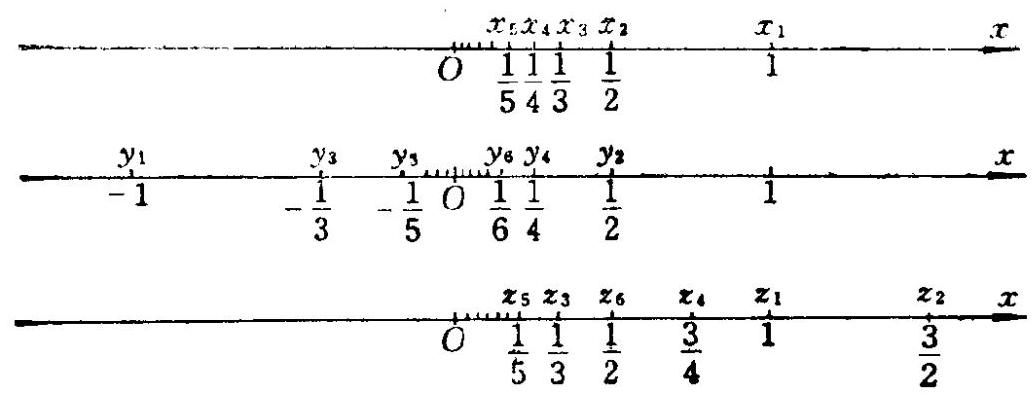
\includegraphics[max width=0.9\textwidth]{images/bo_d25ksc77aajc738obdgg_77_329_373_1036_397_0.jpg}
\end{center}
\hspace*{3em} 

图 3-1

例 3 证明: 实数序列 $\left\{  {1 + {\left( -1\right) }^{n}}\right\}$ 发散.

事实上, $\forall a \in  \mathbf{R}$ ,由
\begin{align*}
	&2 = \left| {2 - a + a}\right|  \leq  \left| {2 - a}\right|  + \left| a\right|\\
	&= \left| {1 + {\left( -1\right) }^{2n} - a}\right|  + \left| {1 + {\left( -1\right) }^{{2n} - 1} - a}\right|
\end{align*}

推知 $\left| {1 + {\left( -1\right) }^{2n} - a}\right|  \geq  1$ 或 $\left| {1 + {\left( -1\right) }^{{2n} - 1} - a}\right|  \geq  1$ ,因此
\begin{align*}
	&\left( {\forall a \in  \mathbf{R}}\right) \left( {\exists {\varepsilon }_{a} = 1 > 0}\right) \left( {\forall n \in  \mathbf{N}}\right) (\exists {2n} \in  \mathbf{N}\text{ 或 }{2n} - 1 \in  \mathbf{N},\\
	&{2n},{2n} - 1 \geq  n)\\
	&\Rightarrow  \left| {1 + {\left( -1\right) }^{2n} - a}\right|  \geq  1\text{ 或 }\\
	&\left| {1 + {\left( -1\right) }^{{2n} - 1} - a}\right|  \geq  1,
\end{align*}

此即表明 $\left\langle  {1 + {\left( -1\right) }^{n}}\right\rangle$ 发散.

直接从序列极限的定义可推出下述等价命题成立:
\begin{align*}
	&\lim {x}_{n} = a \Leftrightarrow  \left( {\forall \varepsilon  > 0}\right) \left( {\exists N \in  \mathbf{N}}\right) \left( {\forall n \in  \mathbf{N},n \geq  N}\right)\\
	&\Rightarrow  \left| {{x}_{n} - a}\right|  \leq  {M\varepsilon }.
\end{align*}

这里 $M$ 是与 $n$ 无关的正数.

熟悉这一点, 将给我们今后证明序列的极限带来方便.

现在我们介绍几个常用的方法.

\section*{2. 用 $\varepsilon  - N$ 极限语言证明序列极限的方法}

直接用 $\varepsilon  - N$ 极限语言证明 $\mathop{\lim }\limits_{{n \rightarrow  \infty }}{x}_{n} = a$ 没有 万能的 方法,总的原则是将差式 $\left| {{x}_{n} - a}\right|$ 适当地放大成 $\left| {{x}_{n} - a}\right|  \leq  {A}_{n}$ 的形式,使得表达式 ${A}_{n}$ 的形式尽可能的简洁,并由 ${A}_{n} < \varepsilon$ 可方便地求出极限定义中所指的自然数 $N$ .

下面就是几个一般的证明方法.

1)直接变形求 ${A}_{n}$ 。

例 4 证明: $\mathop{\lim }\limits_{{n \rightarrow   + \infty }}\sqrt[3]{n}\left( {\sqrt[3]{n} - \sqrt[3]{n - 1}}\right)  = 0$ .

$\forall n \in  \mathbf{N}$ ,由于
\begin{align*}
	&\left| {\sqrt[8]{n}\left( {\sqrt[3]{n} - \sqrt[3]{n - 1}}\right)  - 0}\right|\\
	&= \sqrt[3]{n}\left( {\sqrt[3]{n} - \sqrt[3]{n - 1}}\right)\\
	&= \frac{\sqrt[3]{n}\left( {\sqrt[3]{n} - \sqrt[3]{n - 1}}\right) \left( {\sqrt[3]{{n}^{2}} + \sqrt[3]{n\left( {n - 1}\right) } + \sqrt[3]{{\left( n - 1\right) }^{2}}}\right) }{\sqrt[3]{{n}^{2}} + \sqrt[3]{n\left( {n - 1}\right) } + \sqrt[3]{{\left( n - 1\right) }^{2}}}\\
	&= \frac{3\sqrt{n}}{3\sqrt{{n}^{2}} + \sqrt[3]{n\left( {n - 1}\right) } + \sqrt[3]{{\left( n - 1\right) }^{2}}}
\end{align*}

故 $\forall \varepsilon  > 0$ ,由 $\frac{1}{\sqrt[3]{n}} < \varepsilon$ 得到 $n > \frac{1}{{\varepsilon }^{3}}$ . 令 $N = \left\lbrack  \frac{1}{{\varepsilon }^{3}}\right\rbrack   + 1$ ,则
$$\forall n \in  \mathbf{N},n \geq  N \Rightarrow  \left| {\sqrt[3]{n}\left( {\sqrt[3]{n} - \sqrt[3]{n - 1}}\right)  - 0}\right|  < \frac{1}{\sqrt[3]{n}} < \bar{\varepsilon }.$$

因此 $\mathop{\lim }\limits_{{n \rightarrow   + \infty }}\sqrt[3]{n}\left( {\sqrt[3]{n} - \sqrt[3]{n - 1}}\right)  = 0$ .

例 5 证明: $\mathop{\lim }\limits_{{n \rightarrow   + \infty }}\left( {\frac{1}{1 \cdot  2} + \frac{1}{2 \cdot  3} + \cdots  + \frac{1}{n\left( {n + 1}\right) }}\right)  = 1$ .

$\forall n \in  \mathbf{N}$ ,由于
\begin{align*}
	&\frac{1}{1 \cdot  2} + \frac{1}{2 \cdot  3} + \cdots  + \frac{1}{n\left( {n + 1}\right) } = \left( {1 - \frac{1}{2}}\right)  + \left( {\frac{1}{2} - \frac{1}{3}}\right)\\
	&+ \cdots  + \left( {\frac{1}{n} - \frac{1}{n + 1}}\right)\\
	&= 1 - \frac{1}{n + 1}
\end{align*}

故
$$\left| {\frac{1}{1 \cdot  2} + \frac{1}{2 \cdot  3} + \cdots  + \frac{1}{n\left( {n + 1}\right) } - 1}\right|  = \frac{1}{n + 1} < \frac{1}{n}.$$

$\forall \varepsilon  > 0$ ,由 $\frac{1}{n} < \varepsilon$ 得到 $n > \frac{1}{\varepsilon }$ . 令 $N = \left\lbrack  \frac{1}{\varepsilon }\right\rbrack   + 1$ ,则
$$\forall n \in  N,n \geq  N \Rightarrow  \left| {\frac{1}{1 \cdot  2} + \frac{1}{2 \cdot  3} + \cdots  + \frac{1}{n\left( {n + 1}\right) } - 1}\right|  < \bar{\varepsilon }.$$

因此 $\mathop{\lim }\limits_{{n \rightarrow   + \infty }}\left( {\frac{1}{1 \cdot  2} + \frac{1}{2 \cdot  3} + \cdots  + \frac{1}{n\left( {n + 1}\right) }}\right)  = 1$ .

2) 利用不等式求 ${\mathbf{A}}_{n}$ .

例 6 证明: $\mathop{\lim }\limits_{{n \rightarrow   + \infty }}\frac{1 \cdot  3 \cdot  \cdots  \cdot  \left( {{2n} - 1}\right) }{2 \cdot  4 \cdot  \cdots  \cdot  {2n}} = 0$ .

由不等式 $\frac{a + b}{2} \geq  \sqrt{ab}\left( {a \geq  0,b \geq  0}\right)$ 得到
\begin{align*}
	&2 = \frac{1 + 3}{2} \geq  \sqrt{1 \cdot  3},\;4 = \frac{3 + 5}{2} \geq  \sqrt{3 \cdot  5},\cdots ,\\
	&{2n} = \frac{\left( {{2n} - 1}\right)  + \left( {{2n} + 1}\right) }{2} \geq  \sqrt{\left( {{2n} - 1}\right) \left( {{2n} + 1}\right) }.
\end{align*}

将这些不等式相乘得
\begin{align*}
	&2 \cdot  4 \cdot  \cdots  \cdot  {2n} \geq  \sqrt{1 \cdot  3} \cdot  \sqrt{3 \cdot  5} \cdot  \cdots  \cdot  \sqrt{\left( {{2n} - 1}\right) \left( {{2n} + 1}\right) }\\
	&= 1 \cdot  3 \cdot  \cdots  \cdot  \left( {{2n} - 1}\right) \sqrt{{2n} + 1}.
\end{align*}

由此得到
$$\frac{1 \cdot  3 \cdot  \cdots  \cdot  \left( {{2n} - 1}\right) }{2 \cdot  4 \cdot  \cdots  \cdot  {2n}} < \frac{1}{\sqrt{{2n} + 1}} < \frac{1}{\sqrt{n}}.$$

$\forall \varepsilon  > 0$ ,由 $\frac{1}{\sqrt{n}} < \varepsilon$ 得到 $n > \frac{1}{{\varepsilon }^{2}}$ . 令 $N = \left\lbrack  \frac{1}{{\varepsilon }^{2}}\right\rbrack   + 1$ ,则
$$\forall n \in  N,n \geq  N \Rightarrow  \left| {\frac{1 \cdot  3 \cdot  \cdots  \cdot  \left( {{2n} - 1}\right) }{2 \cdot  4 \cdot  \cdots  \cdot  {2n}} - 0}\right|  < \frac{1}{\sqrt{n}} < \bar{\varepsilon }.$$

因此 $\mathop{\lim }\limits_{{n \rightarrow   + \infty }}\frac{1 \cdot  3 \cdot  \cdots  \cdot  \left( {{2n} - 1}\right) }{2 \cdot  4 \cdot  \cdots  \cdot  {2n}} = 0$ .

例 7 证明: $\mathop{\lim }\limits_{{n \rightarrow   + \infty }}\frac{1}{\sqrt[n]{n!}} = 0$ .

由于 $\forall n \in  \mathbf{N}$ ,

${\left( n!\right) }^{2} = n! \cdot  n!$
$$= 1 \cdot  n \cdot  2 \cdot  \left( {n - 1}\right)  \cdot  \cdots  \cdot  k\left( {n - k + 1}\right)  \cdot  \cdots  \cdot  n \cdot  1,$$

并且 $\forall k,n \in  \mathbf{N},k \leq  n$ 有 $k\left( {n - k + 1}\right)  \geq  n$ ,故
$${\left( n!\right) }^{2} \geq  n \cdot  n \cdot  \cdots  \cdot  n \cdot  \cdots  \cdot  n = {n}^{n}\text{ . }$$

由此推得 $\sqrt[n]{n!} \geq  \sqrt{n}$ 或
$$\frac{1}{\sqrt[n]{n!}} \leq  \frac{1}{\sqrt{n}}$$

$\forall \varepsilon  > 0$ ,由 $\frac{1}{\sqrt{n}} < \varepsilon$ 得到 $n > \frac{1}{{\varepsilon }^{2}}$ . 令 $N = \left\lbrack  \frac{1}{{\varepsilon }^{2}}\right\rbrack   + 1$ ,则
$$\forall n \in  \mathbf{N},n \geq  N \Rightarrow  \left| {\frac{1}{\sqrt[n]{n!}} - 0}\right|  \leq  \frac{1}{\sqrt{n}} < \bar{\varepsilon }.$$

因此 $\mathop{\lim }\limits_{{n \rightarrow   + \infty }}\frac{1}{\sqrt[n]{n!}} = 0$ .

3) 利用二项式展开求 ${\mathbf{A}}_{n}$ .

例 8 证明: $\forall q \in  \mathbf{R},\left| q\right|  < 1,\mathop{\lim }\limits_{{n \rightarrow   + \infty }}{q}^{n} = 0$ .

若 $q = 0$ ,则结论显然成立. 若 $q \neq  0$ ,则由于 $\left| q\right|  < 1$ 有 $\frac{1}{\left| q\right| } > 1$ . 令 $a = \frac{1}{\left| q\right| } - 1$ ,则 $a > 0$ 并且
$$\left| q\right|  = \frac{1}{1 + a},{\left| q\right| }^{n} = \frac{1}{{\left( 1 + a\right) }^{n}}.$$

由二项式展开公式得到
$${\left( 1 + a\right) }^{n} = 1 + {na} + \frac{n\left( {n - 1}\right) }{2}{a}^{2} + \cdots  + {a}^{n} > {na},$$

所以
$$\left| {{q}^{n} - 0}\right|  = {\left| q\right| }^{n} = \frac{1}{{\left( 1 + a\right) }^{n}} < \frac{1}{na}.$$

$\forall \bar{\varepsilon } > 0$ ,由 $\frac{1}{na} < \varepsilon$ 得到 $n > \frac{1}{a\varepsilon }$ . 令 $N = \left\lbrack  \frac{1}{a\varepsilon }\right\rbrack   + 1$ ,则
$$\forall n \in  \mathbf{N},n \geq  N \Rightarrow  \left| {{q}^{n} - 0}\right|  < \frac{1}{na} < \varepsilon .$$

因此 $\mathop{\lim }\limits_{{n \rightarrow  \infty }}{q}^{n} = 0$ .

例 9 证明: $\forall q \in  \mathbf{R},\left| q\right|  < 1,\mathop{\lim }\limits_{{n \rightarrow   + \infty }}n{q}^{n} = 0$ .

若 $q = 0$ ,则结论显然成立.

若 $q \neq  0$ ,则像上一题一样,令 $a = \frac{1}{\left| q\right| } - 1 > 0$ . 则
$$n{\left| q\right| }^{n} = \frac{n}{{\left( 1 + a\right) }^{n}}\left( {n \in  \mathbf{N}}\right) .$$

由于
$${\left( 1 + a\right) }^{n} = 1 + {na} + \frac{n\left( {n - 1}\right) }{2}{a}^{2} + \cdots  + {a}^{n} > \frac{n\left( {n - 1}\right) }{2}{a}^{2},$$

故
$$\left| {n{q}^{n} - 0}\right|  = n{\left| q\right| }^{n} < \frac{n}{\frac{n\left( {n - 1}\right) }{2}{a}^{2}} = \frac{2}{\left( {n - 1}\right) {a}^{2}}\;\left( {n \geq  2}\right) .$$

$\forall \varepsilon  > 0$ ,由 $\frac{2}{\left( {n - 1}\right) {a}^{2}} < \varepsilon$ 得到 $n > 1 + \frac{2}{{a}^{2}\varepsilon }$ . 令 $N = 1 + \left\lbrack  {1 + \frac{2}{{a}^{2}\varepsilon }}\right\rbrack$ ,

则
$$\forall n \in  \mathbf{N},n \geq  N \Rightarrow  \left| {n{q}^{n} - 0}\right|  < \frac{2}{\left( {n - 1}\right) {a}^{2}} < \bar{\varepsilon }.$$

因此 $\mathop{\lim }\limits_{{n \rightarrow   + \infty }}n{q}^{n} = 0$ .

4) 分析法求 ${A}_{n}$

例10 证明: $\mathop{\lim }\limits_{{n \rightarrow   + \infty }}\frac{{a}^{n}}{n!} = 0\left( {a \neq  0}\right)$ .

首先 $\forall n,m \in  \mathbf{N}$ 且 $m \leq  n$ ,我们有
\begin{align*}
	&\left| {\frac{{a}^{n}}{n!} - 0}\right|  = \frac{{\left| a\right| }^{n}}{n!}\\
	&= \left( {\frac{\left| a\right| }{1} \cdot  \frac{\left| a\right| }{2} \cdot  \cdots  \cdot  \frac{\left| a\right| }{m - 1}}\right)  \cdot  \left( {\frac{\left| a\right| }{m} \cdot  \cdots  \cdot  \frac{\left| a\right| }{n - 1}}\right)  \cdot  \frac{\left| a\right| }{n}.
\end{align*}

若取 $m \geq  \left| a\right|$ ,则
$$\left| {\frac{{a}^{n}}{n!} - 0}\right|  < \frac{{\left| a\right| }^{m - 1}}{\left( {m - 1}\right) !} \cdot  1 \cdot  \cdots  \cdot  1 \cdot  \frac{\left| a\right| }{n} = \frac{M}{n}.$$

这里 $M = \frac{{\left| a\right| }^{m}}{\left( {m - 1}\right) !} > 0$ . $\forall \varepsilon  > 0$ ,由 $\frac{M}{n} < \varepsilon$ 得到 $n > \frac{M}{\varepsilon }$ ,令 $N =$  $\max \left( {m,\left\lbrack  \frac{M}{\varepsilon }\right\rbrack   + 1}\right)$ ,则
$$\forall n \in  \mathbf{N},n \geq  N \Rightarrow  \left| {\frac{{a}^{n}}{n!} - 0}\right|  < \frac{M}{n} < \varepsilon .$$

因此 $\mathop{\lim }\limits_{{n \rightarrow   + \infty }}\frac{{a}^{n}}{n!} = 0$ .

例11 证明: 若 $\mathop{\lim }\limits_{{n \rightarrow   + \infty }}{x}_{n} = a$ ,则 $\mathop{\lim }\limits_{{n \rightarrow   + \infty }}\frac{{x}_{1} + {x}_{2} + \cdots  + {x}_{n}}{n} = a$ .

由于 $\mathop{\lim }\limits_{{n \rightarrow   + \infty }}{x}_{n} = a$ ,故由定义
$$\left( {\forall \varepsilon  > 0}\right) \left( {\exists {N}_{1} \in  \mathbf{N}}\right) \left( {\forall n \in  \mathbf{N},n \geq  {N}_{1}}\right)  \Rightarrow  \left| {{x}_{n} - a}\right|  < \frac{\bar{\varepsilon }}{2}.$$

因此 $\forall n \geq  {N}_{1}$ ,
\begin{align*}
	&\left| {\frac{{x}_{1} + {x}_{2} + \cdots  + {x}_{n}}{n} - a}\right|  = \left| \frac{{x}_{1} + {x}_{2} + \cdots  + {x}_{n} - {na}}{n}\right|\\
	&\leq  \left| \frac{\left( {{x}_{1} - a}\right)  + \cdots  + \left( {{x}_{{N}_{1}} - a}\right) }{n}\right|\\
	&+ \left| \frac{\left( {{x}_{{N}_{1} + 1} - a}\right)  + \cdots  + \left( {{x}_{n} - a}\right) }{n}\right|\\
	&< \frac{\left| \left( {x}_{1} - a\right)  + \cdots  + \left( {x}_{{N}_{1}} - a\right) \right| }{n}\\
	&+ \frac{n - {N}_{1}}{n} \cdot  \frac{\varepsilon }{2}\\
	&< \frac{M}{n} + \frac{\varepsilon }{2}
\end{align*}

这里 $M = \left| {\left( {{x}_{1} - a}\right)  + \cdots  + \left( {{x}_{{N}_{1}} - a}\right) }\right|  \geq  0$ . 由 $\frac{M}{n} < \frac{\bar{\varepsilon }}{2}$ 得到 $n$

$> \frac{2M}{\varepsilon }$ . 令 $N = \max \left( {{N}_{1},\left\lbrack  \frac{2M}{\varepsilon }\right\rbrack   + 1}\right)$ ,则
\begin{align*}
	&\forall n \in  N,n \geq  N \Rightarrow  \left| {\frac{{x}_{1} + {x}_{2} + \cdots  + {x}_{n}}{n} - a}\right|  < \frac{M}{n} + \frac{\bar{\varepsilon }}{2}\\
	&< \frac{\varepsilon }{2} + \frac{\varepsilon }{2} = \bar{\varepsilon }
\end{align*}

因此 $\mathop{\lim }\limits_{{n \rightarrow   + \infty }}\frac{{x}_{1} + {x}_{2} + \cdots  + {x}_{n}}{n} = a$ .

\section*{习 题}

1. 证明下列结论等价:

1) $\mathop{\lim }\limits_{{n \rightarrow   + \infty }}{x}_{n} = a$ ;

2) $\left( {\forall \varepsilon  > 0}\right) \left( {\exists N \in  \mathbf{N}}\right) \left( {\forall n \in  \mathbf{N},n \geq  N}\right)  \Rightarrow  \left| {{x}_{n} - a}\right|  < {M\varepsilon }$

(M为常数);

3) $\left( {\forall k \in  \mathbf{N}}\right) \left( {\exists N \in  \mathbf{N}}\right) \left( {\forall n \in  \mathbf{N},n \geq  N}\right)$
$$\Rightarrow  \left| {{x}_{n} - a}\right|  < \frac{1}{k}\text{ . }$$

2. 证明: 实数序列 $\left\langle  {\left( -1\right) }^{n}\right\rangle$ 发散.

3. 证明: $\forall a \in  \mathrm{R},\mathop{\lim }\limits_{{n \rightarrow   + \infty }}\frac{\left\lbrack  na\right\rbrack  }{n} = a$ .

4. 证明: 若 $\mathop{\lim }\limits_{{n \rightarrow   + \infty }}{x}_{n} = a$ ,则 $\mathop{\lim }\limits_{{n \rightarrow   + \infty }}\left| {x}_{n}\right|  = \left| a\right|$ . 举例说明逆命题不成立.

5. 证明: $\mathop{\lim }\limits_{{n \rightarrow   + \infty }}{x}_{n} = a$ 当且仅当 $\mathop{\lim }\limits_{{n \rightarrow   + \infty }}{x}_{2n} = \mathop{\lim }\limits_{{n \rightarrow   + \infty }}{x}_{{2n} + 1} = a$ .

6. 用 $\varepsilon  - N$ 语言证明下列各极限:

1) $\mathop{\lim }\limits_{{n \rightarrow   + \infty }}\frac{n!}{{n}^{n}} = 0$ ,

2) $\mathop{\lim }\limits_{{n \rightarrow   + \infty }}\sqrt[n]{a} = 1\;\left( {a > 0}\right)$ ,

3) $\mathop{\lim }\limits_{{n \rightarrow   + \infty }}\frac{{n}^{k}}{{a}^{n}} = 0\;\left( {a > 1,k \in  \mathbf{N}}\right)$ ,

4) $\mathop{\lim }\limits_{{n \rightarrow   + \infty }}\sqrt[n]{{n}^{k}} = 1\;\left( {k \in  \mathrm{N}}\right)$ ,

5) $\mathop{\lim }\limits_{{n \rightarrow   + \infty }}{\left( k\sqrt{n}\right) }^{\frac{1}{n}} = 1\;\left( {k \in  \mathrm{N}}\right)$ ,

6) $\mathop{\lim }\limits_{{n \rightarrow   + \infty }}\left( {\frac{1}{{n}^{2}} + \frac{1}{{\left( n + 1\right) }^{2}} + \cdots  + \frac{1}{{\left( 2n\right) }^{2}}}\right)  = 0$ ,

7) $\mathop{\lim }\limits_{{n \rightarrow   + \infty }}\left( {\frac{1}{{n}^{2}} + \frac{2}{{n}^{2}} + \cdots  + \frac{n}{{n}^{2}}}\right)  = \frac{1}{2}$ ,

8) $\mathop{\lim }\limits_{{n \rightarrow   + \infty }}\left( {\frac{1}{2} + \frac{2}{{2}^{2}} + \cdots  + \frac{n}{{2}^{n}}}\right)  = 2$ ,

9) $\mathop{\lim }\limits_{{n \rightarrow   + \infty }}\frac{3}{2} \cdot  \frac{5}{4}\cdots \frac{{2}^{{2}^{n}} + 1}{{2}^{{2}^{n}}} = 2$ ,

10) $\mathop{\lim }\limits_{{n \rightarrow   + \infty }}\left( {\frac{1}{2} + \frac{3}{{2}^{2}} + \cdots \cdots  + \frac{{2n} - 1}{{2}^{n}}}\right)  = 3$ .

7. 设 $\left\langle  {x}_{n}\right\rangle$ 是任一实数序列,使得 $\mathop{\lim }\limits_{{n \rightarrow   + \infty }}\left( {{x}_{n + 1} - {x}_{n}}\right)  = 0$ . 证明:
$$\mathop{\lim }\limits_{{n \rightarrow   + \infty }} - \frac{{x}_{n}}{n} = 0$$

8. 设 ${a}_{0},{a}_{1},\cdots ,{a}_{k} \in  \mathrm{R}$ 使得 ${a}_{0} + {a}_{1} + \cdots  + {a}_{k} = 0$ 。证明:
$$\mathop{\lim }\limits_{{n \rightarrow   + \infty }}\left( {{a}_{0}\sqrt{n} + {a}_{1}\sqrt{n + 1} + \cdots  + {a}_{k}\sqrt{n + k}}\right)  = 0.$$

9. 设 $\left\langle  {x}_{n}\right\rangle$ 是任一实数序列,并且 $\mathop{\lim }\limits_{{n \rightarrow   + \infty }}{x}_{n} = a$ .

1) 证明: $\mathop{\lim }\limits_{{n \rightarrow   + \infty }}\frac{{x}_{1} + 2{x}_{2} + \cdots  + n{x}_{n}}{{n}^{2}} = \frac{a}{2}$ .

2) 利用 1) 之结论计算下列各极限值 $\left( {0 < a < 1}\right)$ :
\begin{align*}
	&\mathop{\lim }\limits_{{n \rightarrow   + \infty }}\frac{1}{{n}^{2}}\left( {a + {2}^{2}{a}^{2} + \cdots  + {n}^{2}{a}^{n}}\right)\\
	&\mathop{\lim }\limits_{{n \rightarrow   + \infty }}\frac{1}{{n}^{2}}\left( {1 + \sqrt{{2}^{3}} + \sqrt[3]{{3}^{4}} + \cdots  + \sqrt[n]{{n}^{n + 1}}}\right) .
\end{align*}

10. 分别利用极限定义及反证法证明序列 $\langle \sin n\rangle$ 发散.

11. 设 $\left\langle  {a}_{n}\right\rangle$ 是一实数序列,令
$${b}_{n} = {a}_{n - 1} + 2{a}_{n}\;\left( {n \in  \mathbf{N},n \geq  2}\right) .$$

证明: 若序列 $\left\langle  {b}_{n}\right\rangle$ 收敛,则序列 $\left\langle  {a}_{n}\right\rangle$ 也收敛,并且 $\mathop{\lim }\limits_{{n \rightarrow   + \infty }}{b}_{n} = \underset{n \rightarrow   + \infty }{{31}\lim }{a}_{n}$ .

12. 设实数序列 $\left\langle  {a}_{n}\right\rangle$ 满足条件: $\mathop{\lim }\limits_{{n \rightarrow   + \infty }}\left( {{a}_{n} - {a}_{n - 2}}\right)  = 0$ . 证明:
$$\mathop{\lim }\limits_{{n \rightarrow   + \infty }}\frac{1}{n}\left( {{a}_{n} - {a}_{n - 1}}\right)  = 0.$$

13. 设 $X \subset  R$ 是任一非空集合. 证明: $X$ 是闭集的充分必要条件是
$$\forall {x}_{n} \in  X\left( {n \in  \mathbf{N}}\right) \text{ 且 }{x}_{n} \rightarrow  x\left( {n \rightarrow   + \infty }\right) \text{ ,则 }x \in  X\text{ . }$$

\section{收敛序列的性质}

\section*{1. 收敛序列的一般性质}

性质 1 如果实数序列 $\left\langle  {x}_{n}\right\rangle$ 收敛,则此序列的极限是唯一的.

证明 设 $\mathop{\lim }\limits_{{n \rightarrow  \infty }}{x}_{n} = a,\mathop{\lim }\limits_{{n \rightarrow   + \infty }}{x}_{n} = b$ 并且 $a \neq  b$ . 于是由 $\mathbf{R}$ 的 Hausdorff分离性,存在 $\delta  > 0$ 使得
$$B\left( {a,\delta }\right)  \cap  B\left( {b,\delta }\right)  = \varnothing .$$

另一方面,对 $\delta  > 0$ ,存在 ${N}_{1},{N}_{2} \in  \mathbf{N}$ ,使得
\begin{align*}
	&\forall n \in  \mathbf{N},n \geq  {N}_{1} \Rightarrow  {x}_{n} \in  B\left( {a,\delta }\right) ,\\
	&\forall n \in  \mathbf{N},n \geq  {N}_{2} \Rightarrow  {x}_{n} \in  B\left( {b,\delta }\right) .
\end{align*}

令 $N = \max \left( {{N}_{1},{N}_{2}}\right)$ ,则
$$\forall n \in  \mathbf{N},n \geq  N \Rightarrow  {x}_{n} \in  B\left( {a,\delta }\right)  \cap  B\left( {b,\delta }\right) .$$

这与 $B\left( {a,\delta }\right)  \cap  B\left( {b,\delta }\right)  = \varnothing$ 相矛盾. 因此 $a = b$ .

性质 2 如果 $\mathop{\lim }\limits_{{n \rightarrow   + \infty }}{x}_{n} = a$ ,则任意改变 $\left\langle  {x}_{n}\right\rangle$ 的有限多项后所得新的实数序列 $\left\langle  {y}_{n}\right\rangle$ 也有 $\mathop{\lim }\limits_{{n \rightarrow   + \infty }}{y}_{n} = a$ .

证明留给读者.

性质 3 如果实数序列 $\left\langle  {x}_{n}\right\rangle$ 收敛,则 $\left\langle  {x}_{n}\right\rangle$ 是有界的. 即

$\left( {\exists M > 0}\right) \left( {\forall n \in  \mathbf{N}}\right)  \Rightarrow  \left| {x}_{n}\right|  \leq  M.$

证明 设 $\mathop{\lim }\limits_{{n \rightarrow   + \infty }}{x}_{n} = a$ . 于是对 $\varepsilon  = 1$ ,存在 $N \in  \mathbf{N}$ ,使得
\begin{align*}
	&\forall n \in  \mathbf{N},n \geq  N \Rightarrow  \left| {{x}_{n} - a}\right|  < 1\\
	&\Rightarrow  \left| {x}_{n}\right|  \leq  \left| {{x}_{n} - a}\right|  + \left| a\right|  < 1 + \left| a\right| \text{ . }
\end{align*}

令 $M = \max \left( {\left| {x}_{1}\right| ,\left| {x}_{2}\right| ,\cdots ,\left| {x}_{N - 1}\right| ,1 + \left| a\right| }\right)$ ,则
$$\forall n \in  \mathbf{N},\left| {x}_{n}\right|  \leq  M.$$

性质 4 如果 $\mathop{\lim }\limits_{{n \rightarrow   + \infty }}{x}_{n} = a$ ,则对任一映射 $k : \mathbf{N} \rightarrow  \mathbf{N},k\left( n\right)  <$  $k\left( {n + 1}\right) ,\forall n \in  \mathbf{N}$ ,也有 $\mathop{\lim }\limits_{{n \rightarrow   + \infty }}{x}_{k\left( n\right) } = a$ .

(序列 $\left\langle  {x}_{k\left( n\right) }\right\rangle$ 称为 $\left\langle  {x}_{n}\right\rangle$ 的子序列, $\left\langle  {x}_{k\left( n\right) }\right\rangle$ 也常记为 $\left\langle  {x}_{{k}_{n}}\right\rangle$ )

证明 因为 $\mathop{\lim }\limits_{{n \rightarrow   + \infty }}{x}_{n} = a$ ,所以由定义,
\begin{align*}
	&\left( {\forall \varepsilon  > 0}\right) \left( {\exists N \in  \mathbf{N}}\right) \left( {\forall n \in  \mathbf{N},n \geq  N}\right)\\
	&\Rightarrow  \left| {{x}_{n} - a}\right|  < \varepsilon \text{ . }
\end{align*}

现设 $k : \mathbf{N} \rightarrow  \mathbf{N}$ 是任一映射,满足 $k\left( n\right)  < k\left( {n + 1}\right) ,\forall n \in  \mathbf{N}$ (这种映射称为严格单调上升映射). 那末由归纳法可证:

$\forall n \in  \mathbf{N},k\left( n\right)  \geq  n$ . 由此推得
\begin{align*}
	&\forall n \in  \mathbf{N},n \geq  N \Rightarrow  k\left( n\right)  > N\\
	&\Rightarrow  \left| {{x}_{k\left( n\right) } - a}\right|  < \bar{\varepsilon }\text{ . }
\end{align*}

因此 $\mathop{\lim }\limits_{{n \rightarrow   + \infty }}{x}_{k\left( n\right) } = a$ .

例 1 利用性质 4 证明实数序列 $\left\langle  {1 + {\left( -1\right) }^{n}}\right\rangle$ 发散.

定义严格单调上升映射 $k,l : \mathbf{N} \rightarrow  \mathbf{N}$ 如下:
$$k\left( n\right)  = {2n},l\left( n\right)  = {2n} - 1,\;\forall n \in  \mathbf{N}.$$

那末
$$1 + {\left( -1\right) }^{k\left( n\right) } = 2,1 + {\left( -1\right) }^{l\left( n\right) } = 0\;\forall n \in  \mathbf{N}.$$

因此 $\mathop{\lim }\limits_{{n \rightarrow   + \infty }}\left\lbrack  {1 + {\left( -1\right) }^{k\left( n\right) }}\right\rbrack   = 2,\mathop{\lim }\limits_{{n \rightarrow   + \infty }}\left\lbrack  {1 + {\left( -1\right) }^{l\left( n\right) }}\right\rbrack   = 0$ . 由性质 4 知,序列 $\left\{  {1 + {\left( -1\right) }^{n}}\right\}$ 发散.

例2 设 $p \in  \mathbf{N},\left\langle  {x}_{n}\right\rangle$ 是一实数序列满足 ${x}_{n} = {x}_{n + p}\left( {\forall n \in  \mathbf{N}}\right)$ . 证明,若 $\mathop{\lim }\limits_{{n \rightarrow   + \infty }}{x}_{n} = a$ ,则 ${x}_{n} \equiv  a\;\left( {\forall n \in  \mathbf{N}}\right)$ .

为此,考虑 $p$ 个严格单调上升映射 ${k}^{\left( i\right) } : \mathbf{N} \rightarrow  \mathbf{N}(i = 1,2,\cdots$ , $p)$ ,它定义为:
$${k}^{\left( i\right) }\left( n\right)  = i + \left( {n - 1}\right) p,\;\forall n \in  \mathbf{N}.\;\left( {i = 1,2,\cdots ,p}\right)$$

由于 $\mathop{\lim }\limits_{{n \rightarrow   + \infty }}{x}_{n} = a$ ,故 $\forall i = 1,2,\cdots ,p,\mathop{\lim }\limits_{{n \rightarrow   + \infty }}{x}_{k}{}^{\left( i\right) }{}_{\left( n\right) } = a$ .

另一方面,由假设 ${x}_{n} = {x}_{n + p}\left( {\forall n \in  \mathbf{N}}\right)$ ,我们有
$${x}_{k\left( i\right) \left( n\right) } = {x}_{k\left( i\right) \left( {n + 1}\right) },\;\forall n \in  \mathbf{N}.\;\left( {i = 1,2,\cdots ,p}\right)$$

因此 ${x}_{k\left( i\right) \left( n\right) } \equiv  a\left( {\forall n \in  \mathbf{N}}\right) \left( {i = 1,2,\cdots ,p}\right)$ 从而 ${x}_{n} \equiv  a\left( {\forall n \in  \mathbf{N}}\right)$ .

\section*{2. 收敛序列极限的运算性质}

性质 5 设 $\mathop{\lim }\limits_{{n \rightarrow   + \infty }}{x}_{n} = a,\mathop{\lim }\limits_{{n \rightarrow   + \infty }}{y}_{n} = b$ . 则实数序列 $\left\langle  {{x}_{n} + {y}_{n}}\right\rangle$ , $\left\langle  {{x}_{n}{y}_{n}}\right\rangle  ,\left\langle  \frac{{x}_{n}}{{y}_{n}}\right\rangle  \left( {b \neq  0}\right)$ 也收敛,并且

1) $\mathop{\lim }\limits_{{n \rightarrow   + \infty }}\left( {{x}_{n} + {y}_{n}}\right)  = a + b$ ;

2) $\mathop{\lim }\limits_{{n \rightarrow   + \infty }}{x}_{n}{y}_{n} = {ab}$ ;

3) $\mathop{\lim }\limits_{{n \rightarrow   + \infty }}\frac{{x}_{n}}{{y}_{n}} = \frac{a}{b}\left( {b \neq  0}\right)$ .

证明 因为 $\mathop{\lim }\limits_{{n \rightarrow   + \infty }}{x}_{n} = a,\mathop{\lim }\limits_{{n \rightarrow   + \infty }}{y}_{n} = b$ ,所以
\begin{align*}
	&\left( {\forall \varepsilon  > 0}\right) \left( {\exists N \in  \mathbf{N}}\right) \left( {\forall n \in  \mathbf{N},n \geq  N}\right)\\
	&\Rightarrow  \left\{  \begin{array}{l} \left| {{x}_{n} - a}\right|  < \varepsilon , \\  \left| {{y}_{n} - b}\right|  < \varepsilon ,\left| {y}_{n}\right|  < \left| b\right|  + \varepsilon . \end{array}\right.
\end{align*}

由此推得
\begin{align*}
	&\forall n \in  \mathbf{N},n \geq  N\\
	&\Rightarrow  \left\{  \begin{array}{l} \left| {\left( {{x}_{n} + {y}_{n}}\right)  - \left( {a + b}\right) }\right|  \leq  \left| {{x}_{n} - a}\right|  + \left| {{y}_{n} - b}\right|  < 2\bar{\varepsilon }, \\  \left| {{x}_{n}{y}_{n} - {ab}}\right|  \leq  \left| {y}_{n}\right| \left| {{x}_{n} - a}\right|  + \left| a\right| \left| {{y}_{n} - b}\right|  \end{array}\right.\\
	&< \left( {\left| a\right|  + \left| b\right|  + \varepsilon }\right) \varepsilon .
\end{align*}

因此 $\left\langle  {{x}_{n} + {y}_{n}}\right\rangle$ 及 $\left\langle  {{x}_{n}{y}_{n}}\right\rangle$ 收敛,并且 $\mathop{\lim }\limits_{{n \rightarrow   + \infty }}\left( {{x}_{n} + {y}_{n}}\right)  = a + b$ , $\mathop{\lim }\limits_{{n \rightarrow   + \infty }}{x}_{n}{y}_{n} = {ab}$

若 $b \neq  0$ ,则不妨设 $0 < \varepsilon  < \frac{\left| b\right| }{2}$ ,由 $\left| {{y}_{n} - b}\right|  < \varepsilon$ 推得 $\left| {y}_{n}\right|$  $> \left| b\right|  - \bar{\varepsilon } \geq  \frac{\left| b\right| }{2}\left( {\forall n \in  \mathbf{N},n \geq  N}\right)$ ,因此
\begin{align*}
	&\forall n \in  \mathbf{N},n \geq  N \Rightarrow  \left| {\frac{{x}_{n}}{{y}_{n}} - \frac{a}{b}}\right|\\
	&= \frac{\left| {x}_{n}b - {y}_{n}a\right| }{\left| b\right| \left| {y}_{n}\right| }\\
	&\leq  \frac{2}{{\left| b\right| }^{2}}\left( {\left| {{x}_{n}b - {ab}}\right|  + \left| {{y}_{n}a - {ab}}\right| }\right)\\
	&< \frac{2}{{\left| b\right| }^{2}}\left( {\left| a\right|  + \left| b\right| }\right) \varepsilon
\end{align*}

从而 $\left\langle  \frac{{x}_{n}}{{y}_{n}}\right\rangle$ 收敛,并且 $\mathop{\lim }\limits_{{n \rightarrow   + \infty }}\frac{{x}_{n}}{{y}_{n}} = \frac{a}{b}$ . If

推论 若 $\mathop{\lim }\limits_{{n \rightarrow   + \infty }}{x}_{n} = a,b \in  \mathbf{R}$ ,则
\begin{align*}
	&\mathop{\lim }\limits_{{n \rightarrow   + \infty }}\left( {{x}_{n} + b}\right)  = a + b,\mathop{\lim }\limits_{{n \rightarrow   + \infty }}{x}_{n}b = {ab},\\
	&\mathop{\lim }\limits_{{n \rightarrow   + \infty }}\frac{1}{{x}_{n}} = \frac{1}{a}\left( {a \neq  0}\right) .
\end{align*}

例 3 由于 $\forall p \in  \mathbf{N},\mathop{\lim }\limits_{{n \rightarrow   + \infty }}\frac{1}{{n}^{p}} = 0$ 及
\begin{align*}
	&\frac{{a}_{k}{n}^{k} + {a}_{k - 1}{n}^{k - 1} + \cdots  + {a}_{1}n + {a}_{0}}{{b}_{m}{n}^{m} + {b}_{m - 1}{n}^{m - 1} + \cdots  + {b}_{1}n + {b}_{0}}\\
	&= \frac{{a}_{k} + {a}_{k - 1}\frac{1}{n} + \cdots  + {a}_{1}\frac{1}{{n}^{k - 1}} + {a}_{0}\frac{1}{{n}^{k}}}{{b}_{m} + {b}_{m - 1}\frac{1}{n} + \cdots  + {b}_{1}\frac{1}{{n}^{m - 1}} + {b}_{0}\frac{1}{{n}^{m}}} \cdot  {n}^{k - m},
\end{align*}

因此
\begin{align*}
	&\mathop{\lim }\limits_{{n \rightarrow   + \infty }}\frac{{a}_{k}{n}^{k} + {a}_{k - 1}{n}^{k - 1} + \cdots  + {a}_{1}n + {a}_{0}}{{b}_{m}{n}^{m} + {b}_{m - 1}{n}^{m - 1} + \cdots  + {b}_{1}n + {b}_{0}}\\
	&= \left\{  \begin{array}{ll} \frac{{a}_{k}}{{b}_{m}}, & \text{ 若 }k = m, \\  0, & \text{ 若 }k < m. \end{array}\right.
\end{align*}

从而
\begin{align*}
	&\mathop{\lim }\limits_{{n \rightarrow   + \infty }}\frac{3{n}^{3} - 1}{2{n}^{3} + {n}^{2} + 1} = \frac{3}{2}\\
	&\mathop{\lim }\limits_{{n \rightarrow   + \infty }}\frac{4{n}^{2} + n + 1}{5{n}^{3} + {2n} - 1} = 0.
\end{align*}

\section*{3. 收敛序列的不等式性质}

性质 6 如果 $\mathop{\lim }\limits_{{n \rightarrow   + \infty }}{x}_{n} = a$ ,并且 $a > r\left( {a < r}\right)$ 则

$\left( {\exists N \in  \mathbf{N}}\right) \left( {\forall n \in  \mathbf{N},n \geq  N}\right)  \Rightarrow  {x}_{n} > r\left( {{x}_{n} < r}\right) .$

证明 设 $a > r$ . 由于 $\mathop{\lim }\limits_{{n \rightarrow   + \infty }}{x}_{n} = a$ . 对于 $\varepsilon  = a - r > 0$ ,存在 $N \in  \mathbf{N}$ 使得
\begin{align*}
	&\forall n \in  \mathbf{N},n \geq  N \Rightarrow  \left| {{x}_{n} - a}\right|  < a - r\\
	&\Rightarrow  {x}_{n} > a - \left( {a - r}\right)  = r\text{ . }
\end{align*}

类似可证 $a < r$ 的情形.

性质 7 如果 $\mathop{\lim }\limits_{{n \rightarrow   + \infty }}{x}_{n} = a,\mathop{\lim }\limits_{{n \rightarrow   + \infty }}{y}_{n} = b$ 并且 $a > b\left( {a < b}\right)$ 则

$\left( {\exists N \in  \mathbf{N}}\right) \left( {\forall n \in  \mathbf{N},n \geq  N}\right)  \Rightarrow  {x}_{n} > {y}_{n}\left( {{x}_{n} < {y}_{n}}\right) .$

证明 设 $a > b$ . 于是存在 $r \in  \mathbf{R}$ 使得 $a > r > b$ . 由 $\mathop{\lim }\limits_{{n \rightarrow   + \infty }}{x}_{n} =$  $a > r > b = \mathop{\lim }\limits_{{n \rightarrow   + \infty }}{y}_{n}$ 及性质 6 知,
\begin{align*}
	&\left( {\exists {N}_{1} \in  \mathbf{N}}\right) \left( {\forall n \in  \mathbf{N},n \geq  {N}_{1}}\right)  \Rightarrow  {x}_{n} > r,\\
	&\left( {\exists {N}_{2} \in  \mathbf{N}}\right) \left( {\forall n \in  \mathbf{N},n \geq  {N}_{2}}\right)  \Rightarrow  {y}_{n} < r.
\end{align*}

令 $N = \max \left( {{N}_{1},{N}_{2}}\right)$ ,则
$$\forall n \in  \mathbf{N},n \geq  N \Rightarrow  {x}_{n} > {y}_{n}.$$

对 $a < b$ ,可类似证明.

性质 8 设 $\mathop{\lim }\limits_{{n \rightarrow   + \infty }}{x}_{n} = a,\mathop{\lim }\limits_{{n \rightarrow   + \infty }}{y}_{n} = b$ ,则
$$\forall n \geq  N,{x}_{n} \geq  {y}_{n}\left( {{x}_{n} \leq  {y}_{n}}\right)  \Rightarrow  a \geq  b\left( {a \leq  b}\right) .$$

证明 用反证法, 由性质 7 立即推出.

推论 如果 $\mathop{\lim }\limits_{{n \rightarrow   + \infty }}{x}_{n} = a$ 并且 $\forall n \geq  N,{x}_{n} \geq  r\left( {{x}_{n} \leq  r}\right)$ ,则 $a \geq  r$  $\left( {a \leq  r}\right)$ .

注意 即使在性质 8 中将不等号 “ $\geq  \left(  \leq  \right)$ ” 换成严格不等号 “ $> \left(  < \right)$ ”,也不一定有 $a > b\left( {a < b}\right)$ .

例如,取 ${x}_{n} = \frac{1}{n},{y}_{n} =  - \frac{1}{n}\left( {n \in  \mathbf{N}}\right)$ . 显然有
$${x}_{n} > {y}_{n}\left( {\forall n \in  \mathbf{N}}\right) \text{ ,但是 }\mathop{\lim }\limits_{{n \rightarrow   + \infty }}{x}_{n} = \mathop{\lim }\limits_{{n \rightarrow   + \infty }}{y}_{n} = 0.$$

性质 9 设实数序列 $\left\langle  {x}_{n}\right\rangle  ,\left\langle  {y}_{n}\right\rangle  ,\left\langle  {z}_{n}\right\rangle$ 满足下述条件:

1) ${x}_{n} \leq  {z}_{n} \leq  {y}_{n}\;\left( {\forall n \in  \mathbf{N},n \geq  N}\right)$ ;

2) $\mathop{\lim }\limits_{{n \rightarrow   + \infty }}{x}_{n} = \mathop{\lim }\limits_{{n \rightarrow   + \infty }}{y}_{n} = a$ ,

则 $\mathop{\lim }\limits_{{n \rightarrow   + \infty }}{z}_{n} = a$ .

证明 由于 $\mathop{\lim }\limits_{{n \rightarrow   + \infty }}{x}_{n} = \mathop{\lim }\limits_{{n \rightarrow   + \infty }}{y}_{n} = a$ ,我们有
\begin{align*}
	&\left( {\forall \varepsilon  > 0}\right) \left( {\exists {N}_{0} \in  \mathbf{N},{N}_{0} \geq  N}\right) \left( {\forall n \in  \mathbf{N},n \geq  {N}_{0}}\right)\\
	&\Rightarrow  \left| {{x}_{n} - a}\right|  < \varepsilon ,\left| {{y}_{n} - a}\right|  < \varepsilon .
\end{align*}

由此推得
\begin{align*}
	&\forall n \in  \mathbf{N},n \geq  {N}_{0} \Rightarrow  a - \varepsilon  < {x}_{n},{y}_{n} < a + \overrightarrow{\varepsilon }\\
	&\Rightarrow  a - \varepsilon  < {x}_{n} \leq  {z}_{n} \leq  {y}_{n} < a + \bar{\varepsilon }\\
	&\Rightarrow  \left| {{z}_{n} - a}\right|  < \varepsilon \text{ . }
\end{align*}

因此 $\mathop{\lim }\limits_{{n \rightarrow   + \infty }}{z}_{n} = a$ .

性质 9 常称为序列极限的两边夹法则.

例 4 设 ${x}_{n} = \frac{n}{\sqrt{{n}^{2} + n}},{y}_{n} = \frac{n}{\sqrt{{n}^{2} + 1}}$ ,
$${z}_{n} = \frac{1}{\sqrt{{n}^{2} + 1}} + \frac{1}{\sqrt{{n}^{2} + 2}} + \cdots  + \frac{1}{\sqrt{{n}^{2} + n}}.$$

证明: $\mathop{\lim }\limits_{{n \rightarrow   + \infty }}{x}_{n} = \mathop{\lim }\limits_{{n \rightarrow   + \infty }}{y}_{n} = \mathop{\lim }\limits_{{n \rightarrow   + \infty }}{z}_{n} = 1$ .

首先由不等式
$$1 < \sqrt{1 + \frac{1}{{n}^{2}}} \leq  \sqrt{1 + \frac{1}{n}} < 1 + \frac{1}{n}\left( {\forall n \in  \mathbf{N}}\right)$$

及性质 9 推得 $\mathop{\lim }\limits_{{n \rightarrow   + \infty }}\sqrt{1 + \frac{1}{n}} = \mathop{\lim }\limits_{{n \rightarrow   + \infty }}\sqrt{1 + \frac{1}{{n}^{2}}} = 1$ ,因此
\begin{align*}
	&\mathop{\lim }\limits_{{n \rightarrow   + \infty }}{x}_{n} = \mathop{\lim }\limits_{{n \rightarrow   + \infty }}\frac{1}{\sqrt{1 + \frac{1}{n}}} = 1\\
	&\mathop{\lim }\limits_{{n \rightarrow   + \infty }}{y}_{n} = \mathop{\lim }\limits_{{n \rightarrow   + \infty }}\frac{1}{\sqrt{1 + \frac{1}{{n}^{2}}}} = 1.
\end{align*}

另一方面, 由于
\begin{align*}
	&{x}_{n} = \frac{n}{\sqrt{{n}^{2} + n}} = \frac{1}{\sqrt{{n}^{2} + n}} + \frac{1}{\sqrt{{n}^{2} + n}}\\
	&+ \cdots  + \frac{1}{\sqrt{{n}^{2} + n}}\\
	&< \frac{1}{\sqrt{{n}^{2} + 1}} + \frac{1}{\sqrt{{n}^{2} + 2}} + \cdots\\
	&+ \frac{1}{\sqrt{{n}^{2} + n}} < \frac{n}{\sqrt{{n}^{2} + 1}} = {y}_{n},
\end{align*}

故 ${x}_{n} \leq  {z}_{n} \leq  {y}_{n}\left( {\forall n \in  \mathbf{N}}\right)$ . 从而由性质 9 得到
$$\mathop{\lim }\limits_{{n \rightarrow   + \infty }}{z}_{n} = 1$$

例 5 设 $\left\langle  {x}_{n}\right\rangle$ 是任一实数序列,并且 ${x}_{n} \leq  {x}_{n + 1}\left( {\forall n \in  \mathbf{N}}\right)$ . 证

明: 若 $\mathop{\lim }\limits_{{n \rightarrow   + \infty }}\frac{{x}_{1} + {x}_{2} + \cdots  + {x}_{n}}{n} = a$ ,则 $\mathop{\lim }\limits_{{n \rightarrow   + \infty }}{x}_{n} = a$ .

首先由 ${x}_{n} \leq  {x}_{n + 1}\left( {\forall n \in  \mathbf{N}}\right)$ 我们有
$${y}_{n} =  - \frac{{x}_{1} + {x}_{2} + \cdots  + {x}_{n}}{n} \leq  {x}_{n}\;\left( {\forall n \in  \mathbf{N}}\right) .$$

现在任意固定 $n \in  \mathbf{N}.\forall m \geq  n$ ,
\begin{align*}
	&{y}_{m} = \frac{{x}_{1} + {x}_{2} + \cdots  + {x}_{n} + {x}_{n + 1} + \cdots  + {x}_{m}}{m}\\
	&= \frac{{x}_{1} + {x}_{2} + \cdots  + {x}_{n}}{m} + \frac{{x}_{n + 1} + \cdots  + {x}_{m}}{m}\\
	&\geq  \frac{{x}_{1} + \cdots  + {x}_{n}}{m} + \left( \frac{m - n}{m}\right) {x}_{n}.
\end{align*}

两边令 $m \rightarrow   + \infty$ ,由性质 8 得到
\begin{align*}
	&a = \mathop{\lim }\limits_{{m \rightarrow   + \infty }}{y}_{m} \geq  \mathop{\lim }\limits_{{m \rightarrow   + \infty }}\frac{{x}_{1} + \cdots  + {x}_{n}}{m}\\
	&+ \mathop{\lim }\limits_{{m \rightarrow   + \infty }}\left( \frac{m - n}{m}\right) {x}_{n} = {x}_{n}.
\end{align*}

\section*{由此得到不等式}
$${y}_{n} \leq  {x}_{n} \leq  a\;\left( {\forall n \in  \mathbf{N}}\right) .$$

由于 $\mathop{\lim }\limits_{{n \rightarrow   + \infty }}{y}_{n} = a$ ,故由性质 9 立即推得 $\mathop{\lim }\limits_{{n \rightarrow   + \infty }}{x}_{n} = a$ .

\section*{习 题}

1. 设 $\left\langle  {x}_{n}\right\rangle$ 是任一实数序列满足条件 ${x}_{n} \leq  {x}_{n + 1}\left( {\forall n \in  \mathrm{N}}\right)$ 或 ${x}_{n} \geq  {x}_{n + 1}$  $\left( {\forall n \in  \mathrm{N}}\right)$ 。如果存在 $\left\langle  {x}_{n}\right\rangle$ 的一个子序列 $\left\langle  {x}_{k\left( n\right) }\right\rangle$ 使得 $\mathop{\lim }\limits_{{n \rightarrow   + \infty }}{x}_{k\left( n\right) } = a$ ,则 $\mathop{\lim }\limits_{{n \rightarrow   + \infty }}{x}_{n} = a.$

2. 计算下列各极限

1) $\mathop{\lim }\limits_{{n \rightarrow   + \infty }}\frac{\sqrt{n}}{\sqrt{n + \sqrt{n + \sqrt{n}}}},\; -$

2) $\mathop{\lim }\limits_{{n \rightarrow   + \infty }}\left( {\sqrt{n + 1} - \sqrt{n}}\right) \sqrt{n}$ ,

3) $\mathop{\lim }\limits_{{n \rightarrow   + \infty }}\frac{\sqrt[8]{{n}^{2} + 1}}{n + 2}$

4) $\mathop{\lim }\limits_{{n \rightarrow   + \infty }}\left( {\frac{1}{1 \cdot  3} + \frac{1}{2 \cdot  4} + \cdots  + \frac{1}{n\left( {n + 2}\right) }}\right)$ ,

5) $\mathop{\lim }\limits_{{n \rightarrow   + \infty }}\mathop{\sum }\limits_{{k = 1}}^{n}\frac{1}{\left( {k + p}\right) \left( {k + p + q}\right) }\left( {p,q \in  \mathrm{N}}\right)$ ,

6) $\mathop{\lim }\limits_{{n \rightarrow   + \infty }}\mathop{\sum }\limits_{{k = 1}}^{n}\frac{1}{k\left( {k + 1}\right) \left( {k + 2}\right) }$ .

3. 设 $\mathop{\lim }\limits_{{n \rightarrow   + \infty }}{a}_{n} = a,\mathop{\lim }\limits_{{n \rightarrow   + \infty }}{b}_{n} = b$ . 证明:

1) $\mathop{\lim }\limits_{{n \rightarrow   + \infty }}\max \left( {{a}_{n},{b}_{n}}\right)  = \max \left( {a,b}\right)$ ,

2) $\mathop{\lim }\limits_{{n \rightarrow   + \infty }}\min \left( {{a}_{n},{b}_{n}}\right)  = \min \left( {a,b}\right)$ .

4. 设 $\left\langle  {a}_{n}\right\rangle$ 是任一严格正的实数序列,并且 $\mathop{\lim }\limits_{{n \rightarrow   + \infty }}{a}_{n} = 0$ . 证明:

1) 集合 $\left\{  {n \in  N\mid \forall k \geq  n,{a}_{k} \leq  {a}_{n}}\right\}$ 是无限集.

2) 集合 $\left\{  {n \in  \mathbf{N}\mid \forall k \leq  n,{a}_{n} \leq  {a}_{k}}\right\}$ 是无限集.

5. 设 $\left\langle  {a}_{n}\right\rangle  ,\left\langle  {b}_{n}\right\rangle$ 是任意两个实数序列,并且 $\mathop{\lim }\limits_{{n \rightarrow   + \infty }}{a}_{n} = a,\mathop{\lim }\limits_{{n \rightarrow   + \infty }}{b}_{n} = b$ .

定义序列 $\left\langle  {c}_{n}\right\rangle$ 如下:
$${c}_{n} = \frac{1}{n}\left( {{a}_{1}{b}_{n} + {a}_{2}{b}_{n - 1} + \cdots  + {a}_{n}{b}_{1}}\right) \left( {n \in  \mathbf{N}}\right) .$$

1) 证明: 存在常数 $M > 0$ 使得
$$\left| {{c}_{r} - {ab}}\right|  \leq  \frac{M}{n}\mathop{\sum }\limits_{{i = 1}}^{n}\left( {\left| {{a}_{i} - a}\right|  + \left| {{b}_{i} - b}\right| }\right)$$

2) 证明: $\mathop{\lim }\limits_{{n \rightarrow   + \infty }}{c}_{n} = {ab}$ .

6. 设 $\left\langle  {a}_{n}\right\rangle  ,\left\langle  {b}_{n}\right\rangle$ 是任意两个实数序列,满足:

1) $\mathop{\lim }\limits_{{n \rightarrow   + \infty }}{a}_{n} = 0,\mathop{\lim }\limits_{{n \rightarrow   + \infty }}{b}_{n} = 0$ ;

2) 存在 $M > 0$ 使得 $\forall n \in  \mathbf{N},\left| {b}_{1}\right|  + \left| {b}_{2}\right|  + \cdots  + \left| {b}_{n}\right|  \leq  M$ . 证明:
$$\mathop{\lim }\limits_{{n \rightarrow   + \infty }}\left( {{a}_{1}{b}_{n} + {a}_{2}{b}_{n - 1} + \cdots  + {a}_{n}{b}_{1}}\right)  = 0.$$

7. 试利用两边夹法则证明下列各极限:

1) $\mathop{\lim }\limits_{{n \rightarrow   + \infty }}\left\lbrack  {\frac{1}{{\left( n + 1\right) }^{2}} + \frac{1}{{\left( n + 2\right) }^{2}} + \cdots  + \frac{1}{{\left( 2n\right) }^{2}}}\right\rbrack   = 0$ ,

2) $\mathop{\lim }\limits_{{n \rightarrow   + \infty }}\sqrt[n]{{a}_{1}{}^{n} + {a}_{2}{}^{n} + \cdots  + {a}_{k}{}^{n}} = \mathop{\max }\limits_{{1 \leq  i \leq  k}}\left( {{a}_{i} \geq  0,i = 1,2,\cdots ,k}\right)$ ,

3) $\mathop{\lim }\limits_{{n \rightarrow   + \infty }}\sqrt[n]{\left( \sqrt[n]{n} - 1\right) } = 1$ ,

4) $\mathop{\lim }\limits_{{n \rightarrow   + \infty }}\sqrt[n]{{a}_{1}{a}_{2}\cdots {a}_{n}} = a$ ,这里 ${a}_{n} > 0$ 且 $\mathop{\lim }\limits_{{n \rightarrow   + \infty }}{a}_{n} = a$ .

8. 设 $\left\langle  {x}_{n}\right\rangle$ 是任一实数序列.

1) 证明:如果子序列 $\left\langle  {x}_{2n}\right\rangle  ,\left\langle  {x}_{{2n} + 1}\right\rangle  ,\left\langle  {x}_{3n}\right\rangle$ 收敛,那末序列 $\left\langle  {x}_{n}\right\rangle$ 收敛.

2) 设 $a,b \in  \mathrm{N}$ 是两个互质自然数, $u,v \in  \mathrm{N}$ 使得 ${bv} - {au} = 1$ . 假设子序列 $\left\langle  {x}_{bn}\right\rangle$ 收敛,并且 $\forall r \in  \{ 0,1,\cdots ,a - 1\}$ ,子序列 $\left\langle  {x}_{{an} + r}\right\rangle$ 收敛.

证明: 子序列 $\left\langle  {x}_{bn}\right\rangle  ,\left\langle  {x}_{a :  + r}\right\rangle$ 及 $\left\langle  {x}_{{abn} + b : r}\right\rangle$ 收敛于同一极限 $l$ ,由此推出序列 $\left\langle  {x}_{n}\right\rangle$ 收敛于 $l$ 。

9. 设 $\varphi  : \mathrm{N} \rightarrow  \mathrm{N}$ 是任一严格单调上升映射,并且 $\varphi  = i{d}_{\mathrm{N}}$ .

1) 证明: 存在 $N \in  \mathrm{N}$ 使得 $\forall n \in  \mathrm{N},n \geq  N,\varphi \left( n\right)  > n$ .

2) 记 ${\varphi }^{0} = i{d}_{N}$ ,并归纳地定义 ${\varphi }^{n + 1} = \varphi  \circ  {\varphi }^{n}\left( {\forall n \in  N\cup \{ 0\} }\right)$ ,证明: $\forall n \in  \mathbf{N},n \geq  N,{\varphi }^{k}\left( n\right)  \geq  n + k.\;\left( {k \in  \mathbf{N}}\right)$

3) 设 $\left\langle  {x}_{n}\right\rangle$ 是任一实数序列使得 ${x}_{p\left( n\right) } = {x}_{n}\left( {\forall n \in  N}\right)$ 。证明:如果序列 $\left\langle  {x}_{n}\right\rangle$ 收敛,则从某一项开始, ${x}_{n}$ 为常数.

\section{无穷小、无穷大序列}

有两类特殊的实数序列一一无穷小与无穷大序列一一值得注意.

\section*{1. 无穷小、无穷大序列}

定义 设 $\left\langle  {x}_{n}\right\rangle$ 是任一实数序列.

1) 如果 $\mathop{\lim }\limits_{{n \rightarrow   + \infty }}{x}_{n} = 0$ ,则称 $\left\langle  {x}_{n}\right\rangle$ 是无穷小序列;

2) 如果 $\left\langle  {x}_{n}\right\rangle$ 具有下述性质:
\begin{align*}
	&\left( {\forall M > 0}\right) \left( {\exists N \in  \mathbf{N}}\right) \left( {\forall n \in  \mathbf{N},n \geq  N}\right)\\
	&\Rightarrow  \left| {x}_{n}\right|  > M\text{ , }
\end{align*}

则称 $\left\langle  {x}_{n}\right\rangle$ 是无穷大序列.

特别地, 如果
\begin{align*}
	&\left( {\forall M > 0}\right) \left( {\exists N \in  \mathbf{N}}\right) \left( {\forall n \in  \mathbf{N},n \geq  N}\right)\\
	&\Rightarrow  {x}_{n} > M\left( {{x}_{n} <  - M}\right) ,
\end{align*}

则称 $\left\langle  {x}_{n}\right\rangle$ 是正 (负) 无穷大序列. 有时也称 $\left\langle  {x}_{n}\right\rangle$ 趋于 $+ \infty \left( {-\infty }\right)$ , 并记为
$$\mathop{\lim }\limits_{{n \rightarrow   + \infty }}{x}_{n} =  + \infty \left( {\mathop{\lim }\limits_{{n \rightarrow   + \infty }}{x}_{n} =  - \infty }\right) .$$

例 1 设 $q \in  \mathbf{R}$ . 若 $\left| q\right|  < \left(  > \right) 1$ ,则实数序列 $\left\langle  {q}^{n}\right\rangle$ 是无穷小 (大) 序列.

在 $§1$ 例 8 中我们已经证明了 $\mathop{\lim }\limits_{{n \rightarrow   + \infty }}{q}^{n} = 0\left( {\left| q\right|  < 1}\right)$ ,因此当 $\left| q\right|  < 1$ 时,实数序列 $\left\langle  {q}^{n}\right\rangle$ 是无穷小序列.

现在证明当 $\left| q\right|  > 1$ 时, $\left\langle  {q}^{n}\right\rangle$ 是无穷大序列.

为此令 $\left| q\right|  = 1 + a$ ,则 $a > 0$ . 于是
$$\left| {q}^{n}\right|  = {\left| q\right| }^{n} = {\left( 1 + a\right) }^{n} > {na}.$$

$\forall M > 0$ ,由 ${na} > M$ 得到 $n > \frac{M}{a}$ .

令 $N = \left\lbrack  \frac{M}{a}\right\rbrack   + 1$ ,则
$$\forall n \in  \mathbf{N},n \geq  N \Rightarrow  \left| {q}^{n}\right|  > {na} > M.$$

因此 $\left\langle  {q}^{n}\right\rangle$ 是无穷大序列.

例 $2 \neq  k \in  \mathbf{N}$ ,实数序列 $\left\langle  {n}^{k}\right\rangle$ 与 $\left\langle  {-{n}^{k}}\right\rangle$ 分别是正无穷大序列与负无穷大序列.

\section*{2. 无穷小、无穷大序列的性质}

定理 $3 \cdot  3 \cdot  1$ 设 $\left\langle  {x}_{n}\right\rangle$ 是任一实数序列.

1) 若 $\left\langle  {x}_{n}\right\rangle$ 是无穷小序列,并且 ${x}_{n} \neq  0\left( {\forall n \geq  {N}_{0}}\right)$ 则 $\left\langle  \frac{1}{{x}_{n}}\right\rangle$ 是无穷大序列;

2) 若 $\left\langle  {x}_{n}\right\rangle$ 是无穷大序列,则 $\left\langle  \frac{1}{{x}_{n}}\right\rangle$ 是无穷小序列.

证明 1) 设 $\left\langle  {x}_{n}\right\rangle$ 是无穷小序列并且 ${x}_{n} \neq  0\left( {\forall n \geq  {N}_{0}}\right)$ ,则
\begin{align*}
	&\left( {\forall M > 0}\right) \left( {\exists N \in  \mathbf{N},N \geq  {N}_{0}}\right) \left( {\forall n \in  \mathbf{N},n \geq  N}\right)\\
	&\Rightarrow  \left| {x}_{n}\right|  < \frac{1}{M}\text{ . }
\end{align*}

由此推得
$$\forall n \in  \mathbf{N},n \geq  N \Rightarrow  \left| \frac{1}{{x}_{n}}\right|  > M.$$

因此 $\left\langle  \frac{1}{{x}_{n}}\right\rangle$ 是无穷大序列.

2) 若 $\left\langle  {x}_{n}\right\rangle$ 是无穷大序列. 则由定义
\begin{align*}
	&\left( {\forall \varepsilon  > 0}\right) \left( {\exists N \in  \mathbf{N}}\right) \left( {\forall n \in  \mathbf{N},n \geq  N}\right)\\
	&\Rightarrow  \left| {x}_{n}\right|  > \frac{1}{\varepsilon }\\
	&\Rightarrow  \left| \frac{1}{{x}_{n}}\right|  < \bar{\varepsilon }\text{ . }
\end{align*}

因此 $\left\langle  \frac{1}{{x}_{n}}\right\rangle$ 是无穷小序列.

例 3 由于 $\mathop{\lim }\limits_{{n \rightarrow   + \infty }}\frac{{a}^{n}}{{n}^{n}} = 0\left( {a \neq  0}\right) ,\mathop{\lim }\limits_{{n \rightarrow   + \infty }}n{q}^{n} = 0\;\left( {\left| q\right|  < 1}\right)$ ,故 $\left\langle  \frac{{a}^{n}}{{n}^{n}}\right\rangle$ 与 $\left\langle  {n{q}^{n}}\right\rangle$ 是无穷小序列. 因而 $\left\langle  \frac{{n}^{n}}{{a}^{n}}\right\rangle$ 与 $\left\langle  \frac{1}{n{q}^{n}}\right\rangle$ 是无穷大序列.

定理 $3 \cdot  3 \cdot  2$ 设 $\left\langle  {x}_{n}\right\rangle  ,\left\langle  {y}_{n}\right\rangle$ 是两个实数序列.

1) 若 $\left\langle  {x}_{n}\right\rangle$ 是无穷大序列,则 $\left\langle  {x}_{n}\right\rangle$ 不是有界序列,并且 $\left\langle  {x}_{n}\right\rangle$ 的任意子序列 $\left\langle  {x}_{{k}_{n}}\right\rangle$ 也是无穷大序列.

2) 若 $\left\langle  {x}_{n}\right\rangle$ 是无穷小序列, $\left\langle  {y}_{n}\right\rangle$ 是有界序列,则 $\left\langle  {{x}_{n}{y}_{n}}\right\rangle$ 是无穷小序列.

3) 若 $\mathop{\lim }\limits_{{n \rightarrow   + \infty }}{x}_{n} = a,\left\langle  {y}_{n}\right\rangle$ 是无穷大序列,则 $\left\langle  {{x}_{n} \pm  {y}_{n}}\right\rangle$ 是无穷大序列.

4) 若 $\mathop{\lim }\limits_{{n \rightarrow   + \infty }}{x}_{n} = a,a \neq  0,\left\langle  {y}_{n}\right\rangle$ 是无穷大序列,则 $\left\langle  {{x}_{n}{y}_{n}}\right\rangle$ 是无穷大序列.

证明留给读者作为练习.

上述定理 3.3.2 结论 3 )中若 $\left\langle  {x}_{n}\right\rangle$ 是无穷大序列,则 $\left\langle  {{x}_{n} \pm  }\right.$  $\left. {y}_{n}\right\rangle$ 不一定是无穷大序列,结论 4 ) 中若 $\mathop{\lim }\limits_{{n \rightarrow   + \infty }}{x}_{n} = 0$ ,则 $\left\langle  {{x}_{n}{y}_{n}}\right\rangle$ 也不一定是无穷大序列. 在这两种情况下,当 $n \rightarrow   + \infty$ 时 ${x}_{n} \pm  {y}_{n}$ 与 ${x}_{n}{y}_{n}$ 的变化可出现下述各种情形.

\section*{3. 不定型}

$\infty  - \infty  :$ 若 $\mathop{\lim }\limits_{{n \rightarrow   + \infty }}{x}_{n} =  + \infty ,\mathop{\lim }\limits_{{n \rightarrow   + \infty }}{y}_{n} =  + \infty$ ,则序列 $\left\langle  {{x}_{n} - {y}_{n}}\right\rangle$ 称为 $\infty  - \infty$ 不定型序列. 例如

i) ${x}_{n} = n + \frac{1}{n},{y}_{n} = n\;\left( {n \in  \mathbf{N}}\right)$ ,则
$${x}_{n} - {y}_{n} = \frac{1}{n} \rightarrow  0\;\left( {n \rightarrow   + \infty }\right)$$

ii) ${x}_{n} = {2n},{y}_{n} = n\;\left( {n \in  \mathbf{N}}\right)$ ,则
$${x}_{n} - {y}_{n} = n \rightarrow   + \infty \;\left( {n \rightarrow   + \infty }\right) ;$$

iii) ${x}_{n} = n + {\left( -1\right) }^{n},{y}_{n} = n\;\left( {n \in  \mathbf{N}}\right)$ ,则
$${x}_{n} - {y}_{n} = {\left( -1\right) }^{n}\text{ 发散 }\left( {n \rightarrow   + \infty }\right) \text{ . }$$

$0 \cdot  \infty  :$ 若 $\mathop{\lim }\limits_{{n \rightarrow   + \infty }}{x}_{n} = 0,\mathop{\lim }\limits_{{n \rightarrow   + \infty }}{y}_{n} =  \pm  \infty$ ,则序列 $\left\langle  {{x}_{n}{y}_{n}}\right\rangle$ 称为 $0 \cdot  \infty$ 不定型序列. 例如

i) ${x}_{n} = \frac{1}{n},{y}_{n} = n\;\left( {n \in  \mathbf{N}}\right)$ ,则 ${x}_{n}{y}_{n} \equiv  1.\left( {n \in  \mathbf{N}}\right)$ ;

ii) ${x}_{n} = \frac{1}{n},{y}_{n} = {n}^{2}\;\left( {n \in  \mathrm{N}}\right)$ ,则
$${x}_{n}{y}_{n} = n \rightarrow   + \infty \;\left( {n \rightarrow   + \infty }\right) ;$$

iii) ${x}_{n} = \frac{{\left( -1\right) }^{n}}{n},{y}_{n} = n\;\left( {n \in  \mathbf{N}}\right)$ ,则

${x}_{n}{y}_{n} = {\left( -1\right) }^{n}$ 发散 $\left( {n \rightarrow   + \infty }\right)$ .

$\frac{\infty }{\infty },\;\frac{0}{0} :$ 若 $\mathop{\lim }\limits_{{n \rightarrow   + \infty }}{x}_{n} =  \pm  \infty ,\mathop{\lim }\limits_{{n \rightarrow   + \infty }}{y}_{n} =  \pm  \infty$ 或 $\mathop{\lim }\limits_{{n \rightarrow   + \infty }}{x}_{n} = 0,$

$\mathop{\lim }\limits_{{n \rightarrow   + \infty }}{y}_{n} = 0$ ,则 $\left\langle  \frac{{x}_{n}}{{y}_{n}}\right\rangle$ 称为 $\frac{\infty }{\infty }$ 或 $\frac{0}{0}$ 不定型序列.

这后面两种不定型实际上可化为 $0 \cdot  \infty$ 不定型,因为只需写 $\frac{{x}_{n}}{{y}_{n}}$ 为 $\frac{1}{{x}_{n}} \cdot  {y}_{n}$ 或 ${x}_{n} \cdot  \frac{1}{{y}_{n}}$ 即可.

关于不定型序列的极限计算, 要具体情况具体分析, 目前有一个可供我们使用的方法就是Stolz定理 (见习题5).

\section*{习 题}

1. 设 $\left\langle  {a}_{n}\right\rangle$ 是任一实数序列, ${a}_{n} \geq  0\left( {\forall n \in  \mathbf{N}}\right)$ ,并且存在 $c > 0$ 使得 $\forall m$ 。 $n \in  \mathbf{N},m < n,{a}_{n} \leq  c{a}_{m}$ 。证明:如果 $\left\langle  {a}_{n}\right\rangle$ 有子序列 $\left\langle  {a}_{{k}_{n}}\right\rangle$ 使得
$$\mathop{\lim }\limits_{{n \rightarrow   + \infty }}{a}_{{k}_{n}} = 0,\;\text{ 则 }\mathop{\lim }\limits_{{n \rightarrow   + \infty }}{a}_{n} = 0.$$

2. 设 $\left\langle  {x}_{n}\right\rangle$ 是一个无界实数序列,则从 $\left\langle  {x}_{n}\right\rangle$ 中可以选出一个无穷大子序列. 特别地,如果 $\left\langle  {x}_{n}\right\rangle$ 是无上 (下) 界实数序列,则从 $\left\langle  {x}_{n}\right\rangle$ 中可以选出一个严格单调上升 (下降) 的正 (负) 无穷大子序列.

3. 设 $\left\langle  {a}_{n}\right\rangle$ 是一实数序列 并且 $\mathop{\lim }\limits_{{n \rightarrow   + \infty }}\frac{{a}_{n + 1}}{{a}_{n}} = \lambda ,\left| \lambda \right|  < 1$ ,证明
$$\mathop{\lim }\limits_{{n \rightarrow   + \infty }}{a}_{n} = 0$$

利用此结论证明下列各极限:

1) $\mathop{\lim }\limits_{{n \rightarrow   + \infty }}\frac{{a}^{n}}{n!} = 0\left( {a \in  \mathbf{R}}\right)$ ;

2) $\mathop{\lim }\limits_{{n \rightarrow   + \infty }}\frac{b\left( {b - 1}\right) \cdots \left( {b - n + 1}\right) {a}^{n}}{n!} = 0\left( {\left| a\right|  < 1,b \in  \mathbf{R}}\right)$ ;

3) $\mathop{\lim }\limits_{{n \rightarrow   + \infty }}\frac{{1}^{2} \cdot  {3}^{2}\cdots  \cdot  {\left( 2n - 1\right) }^{2}}{{2}^{2} \cdot  {4}^{2} \cdot  \cdots  \cdot  {\left( 2n\right) }^{2}}{a}^{n} = 0\left( {\left| a\right|  < 1}\right)$ .

4. 设 $\left\langle  {a}_{n}\right\rangle$ 是一正实数序列,并且 $\mathop{\lim }\limits_{{n \rightarrow   + \infty }}\frac{{a}_{n + 1}}{{a}_{n}} = \lambda ,\lambda  > 1$ . 证明
$$\mathop{\lim }\limits_{{n \rightarrow   + \infty }}{a}_{n} =  + \infty \text{ . }$$

利用此结论证明下列各题:

1) $\mathop{\lim }\limits_{{n \rightarrow   + \infty }}\frac{3 \cdot  6 \cdot  9 \cdot  \cdots  \cdot  {3n}}{7 \cdot  {10} \cdot  {13} \cdot  \cdots  \cdot  \left( {{3n} + 4}\right) }{a}^{n} =  + \infty \left( {a > 1}\right)$ ;

2) $\mathop{\lim }\limits_{{n \rightarrow   + \infty }}\frac{1 \cdot  3 \cdot  5 \cdot  \cdots  \cdot  \left( {{2n} - 1}\right) {a}^{2n}}{2 \cdot  4 \cdot  6 \cdot  \cdots  \cdot  \left( {{2n} - 2}\right)  \cdot  {2n}} =  + \infty \left( {\left| a\right|  > 1}\right)$ ;

3) $\mathop{\lim }\limits_{{n \rightarrow   + \infty }}\sqrt{\frac{n - 1}{{n}^{3} - 1}}{a}^{n} =  + \infty \left( {n > 1}\right)$ .

5. 证明下述 Stolz定理:

设 $\left\langle  {x}_{n}\right\rangle  ,\left\langle  {y}_{n}\right\rangle$ 是任意两个实数序列,并且满足条件:

1) ${y}_{n} < {y}_{n + 1}\left( {\forall n \in  \mathbf{N}}\right)$ ;

2) $\mathop{\lim }\limits_{{n \rightarrow   + \infty }}{y}_{n} =  + \infty$ ;

3) $\mathop{\lim }\limits_{{n \rightarrow   + \infty }}\frac{{x}_{n + 1} - {x}_{n}}{{y}_{n + 1} - {y}_{n}} = a \in  R$ 或 $\pm  \infty$ .

则
$$\mathop{\lim }\limits_{{n \rightarrow   + \infty }}\frac{{x}_{n}}{{y}_{n}} = \mathop{\lim }\limits_{{n \rightarrow   + \infty }}\frac{{x}_{n + 1} - {x}_{n}}{{y}_{n + 1} - {y}_{n}}.$$

试利用此结论证明下述各极限:

1) $\mathop{\lim }\limits_{{n \rightarrow   + \infty }}\frac{{n}^{2}}{{a}^{2n}} = 0\left( {\left| a\right|  > 1}\right)$ ;

2) $\mathop{\lim }\limits_{{n \rightarrow   + \infty }}\frac{{1}^{k} + {2}^{k} + \cdots  + {n}^{k}}{{n}^{k + 1}} = \frac{1}{k + 1}\left( {\forall k \in  \mathbf{N}}\right)$ ;

3) $\mathop{\lim }\limits_{{n \rightarrow   + \infty }}\frac{{1}^{k} + {3}^{k} + \cdots  + {\left( 2n + 1\right) }^{k}}{{n}^{k + 1}} = \frac{{2}^{k}}{k + 1}\left( {\forall k \in  \mathbf{N}}\right)$ ;

4) $\mathop{\lim }\limits_{{n \rightarrow   + \infty }}\left( {\frac{{1}^{k} + {2}^{k} + \cdots  + {n}^{k}}{{n}^{k}} - \frac{n}{k + 1}}\right)  = \frac{1}{2}$ ,

5) $\mathop{\lim }\limits_{{n \rightarrow   + \infty }}\frac{{a}_{1} + 2{a}_{2} + \cdots  + n{a}_{n}}{n\left( {n + 1}\right) } =  \pm  \infty ,$ 若 $\mathop{\lim }\limits_{{n \rightarrow   + \infty }}{a}_{n} =  \pm  \infty$ .

6. 设 ${a}_{k} > 0\left( {k \in  \mathbf{N}}\right)$ ,定义序列 $\left\langle  {A}_{n}\right\rangle$ 如下:
$${A}_{n} = {a}_{1} + {a}_{2} + \cdots  + {a}_{n}\left( {\forall n \in  \mathbf{N}}\right) .$$

假设 $\left\langle  {A}_{n}\right\rangle$ 发散,但 $\mathop{\lim }\limits_{{n \rightarrow   + \infty }}{a}_{n}{A}_{n}^{-1} = 0$ . 证明:
$$\mathop{\lim }\limits_{{n \rightarrow   + \infty }}\frac{{a}_{1}{A}_{1}^{-1} + {a}_{2}{A}_{2}^{-1} + \cdots  + {a}_{n}{A}_{n}^{-1}}{\log {A}_{n}} = 1.$$

7. 设 $\left\langle  {a}_{n}\right\rangle  ,\left\langle  {b}_{n}\right\rangle$ 是两个正数序列,并且
\begin{align*}
	&\mathop{\lim }\limits_{{n \rightarrow   + \infty }}\frac{{a}_{1} + {a}_{2} + \cdots  + {a}_{n}}{n{a}_{n}} = a,\\
	&\mathop{\lim }\limits_{{n \rightarrow   + \infty }}\frac{{b}_{1} + {b}_{2} + \cdots  + {b}_{n}}{n{b}_{n}} = b,
\end{align*}

$a + b > 0$ . 证明:
$$\mathop{\lim }\limits_{{n \rightarrow   + \infty }}\frac{{a}_{1}{b}_{1} + 2{a}_{2}{b}_{2} + \cdots  + n{a}_{n}{b}_{n}}{{n}^{2}{a}_{n}{b}_{n}} = \frac{ab}{a + b}.$$

8. 设 $\left\langle  {a}_{n}\right\rangle  ,\left\langle  {b}_{n}\right\rangle$ 是两个实数序列,满足条件:

1) ${b}_{n} < {b}_{n + 1}\left( {\forall n \in  \mathrm{N}}\right) ,\mathop{\lim }\limits_{{n \rightarrow   + \infty }}{b}_{n} =  + \infty$ ;

2) $\mathop{\lim }\limits_{{n \rightarrow   + \infty }}\left( {{a}_{1} + {a}_{2} + \cdots  + {a}_{n}}\right)  = a \in  \mathbf{R}$ .

证明:
$$\mathop{\lim }\limits_{{n \rightarrow   + \infty }}\frac{{a}_{1}{b}_{1} + {a}_{2}{b}_{2} + \cdots  + {a}_{n}{b}_{n}}{{b}_{n}} = 0.$$

\section{实数的连续性}

在第 2 章 $§1$ 例 3 中我们证明了以
$${r}_{n} = 1 + \frac{1}{1!} + \frac{1}{2!} + \cdots  + \frac{1}{n!}\;\left( {n \in  \mathbf{N}}\right)$$

为通项的序列 $\left\langle  {r}_{n}\right\rangle$ 是一个有理数 Cauchy 序列. 下面我们来证明 $\left\langle  {r}_{n}\right\rangle$ 并没有有理数极限.

事实上,由 ${r}_{n}$ 的表达式我们有
\begin{align*}
	&{r}_{n + 1} + \frac{1}{\left( {n + 1}\right) !} = {r}_{n} + \frac{1}{\left( {n + 1}\right) !} + \frac{1}{\left( {n + 1}\right) !}\\
	&= {r}_{n} + \frac{2}{\left( {n + 1}\right) !} < {r}_{n} + \frac{1}{n!}\;\left( {n \geq  2}\right) .
\end{align*}

由此推得 $\forall n \geq  2,\forall k \in  \mathbf{N}$ ,
\begin{align*}
	&{r}_{n} < {r}_{n + 1} < {r}_{n + k} + \frac{1}{\left( {n + k}\right) !}\\
	&< {r}_{n + 1} + \frac{1}{\left( {n + 1}\right) !} < {r}_{n} + \frac{1}{n!}
\end{align*}

如果存在 $\frac{q}{p} \in  \mathbf{Q}$ ,使得 $\mathop{\lim }\limits_{{n \rightarrow  \infty }}{r}_{n} = \frac{q}{p}$ ,则在上述不等式中令 $k$  $\rightarrow   + \infty$ 取极限即得到
$${r}_{n} < \frac{q}{p} < {r}_{n} + \frac{1}{n!}$$

特别取 $n = p$ ,并两边同乘以 $p$ 得到
$$0 < \left( {q - p{r}_{p}}\right) \left( {p - 1}\right) ! < 1$$

这显然是矛盾的,因为 $\left( {q - p{r}_{p}}\right) \left( {p - 1}\right)$ ! 是一个整数.

那末我们要问:序列 $\left\langle  {r}_{n}\right\rangle$ 在实数域 $\mathrm{R}$ 中是否收敛呢? 答案是肯定的. 这一节的目的就是要证明: 每一个实数 Cauchy 序列在 $\mathbf{R}$ 中收敛. 这一性质通常称为 $\mathbf{R}$ 的完备性.

$\mathbf{R}$ 的完备性可以用下列7个定理中的每一个定理独立地刻划:

1 ) Cauchy 收敛准则.

2) 确界存在定理.

3) 单调序列极限存在定理.

4)区间套定理.

5 )聚点定理.

6) Bolzano-Weierstrass定理.

7 ) Cantor有限覆盖定理.

这七个定理也称为实数的连续性定理. 下面我们将按上述顺序证明它们的等价性.

首先我们证明下述引理.

引理 设 $x \in  \mathbf{R}$ . 则对 $x$ 的任一代表 $\left\langle  {x}_{n}\right\rangle$ 有
$$\mathop{\lim }\limits_{{n \rightarrow   + \infty }}{\widetilde{x}}_{n} = x$$

证明 设 $\varepsilon  > 0$ . 根据第 2 章 §2 引理知,存在正有理数 $\alpha$ ,使得 $0 < \widetilde{\alpha } < \varepsilon$ . 由于 $\left\langle  {x}_{n}\right\rangle$ 是有理数 Cauchy 序列,对 $\alpha  > 0$ ,存在 $N \in  \mathbf{N}$ 使得
\begin{align*}
	&\forall n,m \in  \mathbf{N},n,m \geq  N \Rightarrow  \left| {{x}_{n} - {x}_{m}}\right|  < \alpha\\
	&\Rightarrow   - a < {x}_{n} - {x}_{m} < a\text{ . }
\end{align*}

固定 $n \in  \mathbf{N}$ . 令
$${r}_{m} = \left\{  \begin{array}{ll} 0, & \text{ 若 }m = 1,2,\cdots ,N - 1, \\  {x}_{n} - {x}_{m}, & \text{ 若 }m \geq  N. \end{array}\right.$$

则 $\left\langle  {r}_{m}\right\rangle$ 是有理数 Cauchy 序列,并且 ${\widetilde{x}}_{n} - x = \overset{⏜}{\left\langle  {r}_{m}\right\rangle  }$ ,以及
$$- \alpha  < {r}_{m} < \alpha \;\left( {\forall m \in  \mathbf{N}}\right) .$$

根据 $\mathrm{R}$ 的序关系定义,我们有
\begin{align*}
	&\forall n \in  \mathbf{N},n \geq  N \Rightarrow   - \widetilde{\alpha } < \widetilde{{x}_{n}} - x < \widetilde{\alpha }\\
	&\Rightarrow   - \ddot{\varepsilon } < {x}_{n} - x < \bar{\varepsilon }\\
	&\Rightarrow  \left| {\widetilde{{x}_{n}} - x}\right|  < \bar{\varepsilon }\text{ . }
\end{align*}

因此 $\mathop{\lim }\limits_{{n \rightarrow   + \infty }}{x}_{n} = x$ .

\section*{1. Cauchy 收敛准则}

定义 我们称实数序列 $\left\langle  {x}_{n}\right\rangle$ 为Cauchy序列,如果它具有下述性质:
\begin{align*}
	&\left( {\forall \varepsilon  > 0}\right) \left( {\exists N \in  \mathbf{N}}\right) \left( {\forall n,m \in  \mathbf{N},n,m \geq  N}\right)\\
	&\Rightarrow  \left| {{x}_{n} - {x}_{m}}\right|  < \varepsilon \text{ . }
\end{align*}

显然,当 $\left\langle  {x}_{n}\right\rangle$ 为有理数序列时,上述定义与第 2 章 $§1$ 的有理数Cauchy序列定义是一致的.

定理 $3 \cdot  4 \cdot  1$ (Cauchy收敛准则) 实数序列 $\left\langle  {x}_{n}\right\rangle$ 收敛的充分必要条件是 $\left\langle  {x}_{n}\right\rangle$ 为 Cauchy 序列.

证明 必要性 设 $\left\langle  {x}_{n}\right\rangle$ 收敛于 $a$ . 那末
\begin{align*}
	&\left( {\forall \varepsilon  > 0}\right) \left( {\exists N \in  \mathbf{N}}\right) \left( {\forall n \in  \mathbf{N},n \geq  N}\right)\\
	&\Rightarrow  \left| {{x}_{n} - a}\right|  < \varepsilon /2\text{ . }
\end{align*}

因此
\begin{align*}
	&\forall n,m \in  N,n,m \geq  N\\
	&\Rightarrow  \left| {{x}_{n} - {x}_{m}}\right|  < \left| {{x}_{n} - a}\right|  + \left| {{x}_{m} - a}\right|  < \bar{\varepsilon }\text{ . }
\end{align*}

此即表明 $\left\langle  {x}_{n}\right\rangle$ 是 Cauchy 序列.

充分性 设 $\left\langle  {x}_{n}\right\rangle$ 是 Cauchy 序列. 那末
\begin{align*}
	&\left( {\forall \varepsilon  > 0}\right) \left( {\exists {N}_{1} \in  \mathbf{N}}\right) \left( {\forall n,m \in  \mathbf{N},n,m \geq  {N}_{1}}\right)\\
	&\Rightarrow  \left| {{x}_{n} - {x}_{m}}\right|  < \frac{\varepsilon }{3}.
\end{align*}

另一方面,由有理实数集 $\widetilde{\mathbf{Q}}$ 在 $\mathbf{R}$ 中的稠密性,对每一个 ${x}_{n} \in  \mathbf{R}$ ,存在 ${r}_{n} \in  \mathbf{Q}$ ,使得
$$\left| {{x}_{n} - {\widetilde{r}}_{n}}\right|  > \frac{1}{n}\left( {\forall n \in  N}\right) .$$

我们证明由此得到的序列 $\left\langle  {r}_{n}\right\rangle$ 是有理数 Cauchy 序列.

为此,我们注意到 $\overset{⏜}{\left\langle  \frac{1}{n}\right\rangle  } = 0$ ,因此由上述引理知 $\mathop{\lim }\limits_{{n \rightarrow   + \infty }}\frac{1}{n} = 0$ . 从而存在 ${N}_{2} \in  \mathbf{N}$ 使得
$$\forall n,m \in  \mathbf{N},n,m \geq  {N}_{2} \Rightarrow  \frac{\widetilde{1}}{n} < \frac{\varepsilon }{3},\frac{\widetilde{1}}{m} < \frac{\varepsilon }{3}.$$

令 ${N}_{0} = \max \left( {{N}_{1},{N}_{2}}\right)$ ,则
\begin{align*}
	&\forall n,m \in  \mathbf{N},n,m \geq  {N}_{0} \Rightarrow  \left| {{r}_{n} - {r}_{m}}\right|  = \left| {{\widetilde{r}}_{n} - {\widetilde{r}}_{m}}\right|\\
	&\leq  \left| {{\widetilde{r}}_{n} - {x}_{n}}\right|  + \left| {{x}_{n} - {x}_{m}}\right|  + \left| {{x}_{m} - {x}_{m}}\right|\\
	&< \frac{1}{n} + \frac{\varepsilon }{3} + \frac{1}{m}\\
	&< \frac{\varepsilon }{3} + \frac{\varepsilon }{3} + \frac{\varepsilon }{3} = {\bar{\varepsilon }}_{ \circ  }
\end{align*}

现在令 $a = \overset{⏜}{\left\langle  {r}_{n}\right\rangle  }$ ,由上述引理, $\mathop{\lim }\limits_{{n \rightarrow   + \infty }}\overset{⏜}{{r}_{n}} = a$ . 因此存在 ${N}_{3} \in  \mathbf{N}$ 使得
$$\forall n \in  \mathbf{N},n \geq  {N}_{3} \Rightarrow  \left| {{\widetilde{r}}_{n} - a}\right|  < \frac{\bar{\varepsilon }}{3}.$$

最后令 $N = \max \left( {{N}_{0},{N}_{3}}\right)$ . 则
$$\forall n \in  \mathbf{N},n \geq  N \Rightarrow  \left| {{x}_{n} - a}\right|  < \left| {{x}_{n} - {\widetilde{r}}_{n}}\right|  + \left| {{\widetilde{r}}_{n} - a}\right|  < \bar{\varepsilon }\text{ . 因 }$$

此 $\mathop{\lim }\limits_{{n \rightarrow   + \infty }}{x}_{n} = a$ .

例 1 对于本节开头所提的有理数序列 $\left\langle  {r}_{n}\right\rangle$ ......
$${r}_{n} = 1 + \frac{1}{1!} + \frac{1}{2!} + \cdots  + \frac{1}{n!}\left( {n \in  \mathbf{N}}\right) ,$$

由于它是 Cauchy 序列, 故根据 Cauchy 收敛准则, 此序列在 $\mathbf{R}$ 中收敛. 以后我们将知道这个序列的极限就是无理数 $e(e$ 的定义见第 5 章 §4).

例2 设
$${x}_{n} = \frac{1}{{1}^{2}} + \frac{1}{{2}^{2}} + \cdots  + \frac{1}{{n}^{2}}\left( {n \in  \mathbf{N}}\right) .$$

证明实数序列 $\left\langle  {x}_{n}\right\rangle$ 收敛.

根据 Cauchy 收敛准则,我们只需证明 $\left\langle  {x}_{n}\right\rangle$ 是 Cauchy 序列. 事实上, $\forall n,k \in  \mathbf{N}$ ,
\begin{align*}
	&\left| {{x}_{n + k} - {x}_{n}}\right|  = \left| {\frac{1}{{\left( n + 1\right) }^{2}} + \frac{1}{{\left( n + 2\right) }^{2}} + \cdots  + \frac{1}{{\left( n + k\right) }^{2}}}\right|\\
	&< \frac{1}{n\left( {n + 1}\right) } + \frac{1}{\left( {n + 1}\right) \left( {n + 2}\right) } + \cdots\\
	&+ \frac{1}{\left( {n + k - 1}\right) \left( {n + k}\right) }\\
	&= \left( {\frac{1}{n} - \frac{1}{n + 1}}\right)  + \left( {\frac{1}{n + 1} - \frac{1}{n + 2}}\right)  + \cdots\\
	&+ \left( {\frac{1}{n + k - 1} - \frac{1}{n + k}}\right)\\
	&= \frac{1}{n} - \frac{1}{n + k}\\
	&< \frac{1}{n}\text{ . }
\end{align*}

由此我们有
\begin{align*}
	&\left( {\forall \varepsilon  > 0}\right) \left( {\exists N = \left\lbrack  \frac{1}{\varepsilon }\right\rbrack   + 1}\right) \left( {{\forall }_{n},k \in  \mathbf{N},n \geq  N}\right)\\
	&\Rightarrow  \left| {{x}_{n + k} - {x}_{n}}\right|  < \varepsilon \text{ . }
\end{align*}

因此 $\left\langle  {x}_{n}\right\rangle$ 是 Cauchy 序列.

附注 因 $\mathbf{R}$ 的任何一个Cauchy序列都收敛,故我们称实数度量空间 $R$ 是完备度量空间.

Cauchy收敛准则完全是利用实数序列本身的信息来判断序列收敛与否的, 它避免了用极限定义证明序列收敛需预先估计极限数的弊病. 因此在收敛性问题的研究中有着广泛的应用.

\section*{2. 集合的上、下确界}

定义 设 $X \subset  \mathbf{R}$ 是任一集合.

1)我们称 $X$ 是上 (下) 有界集,如果
$$\left( {\exists M \in  \mathbf{R}}\right) \left( {\forall x \in  X}\right)  \Rightarrow  x \leq  M\left( { \geq  M}\right) .$$

$M$ 称为 $X$ 的上 (下) 界.

2) 我们称 $X$ 是有界集,如果 $X$ 既是上有界的,又是下有界的.

由上述定义可知

i) 若 $X$ 是上 (下) 有界集, $M$ 是 $X$ 的一个上 (下) 界,则 所有比 $M$ 大 (小) 的实数 ${M}^{\prime }$ 都是 $X$ 的上 (下) 界.

ii) $X$ 是有界集 $\Leftrightarrow  \exists m,M \in  \mathbf{R},\forall x \in  X,m \leq  x \leq  M$
$$\Leftrightarrow  \exists M \in  {\mathbf{R}}_{ * }^{ + },\;\forall x \in  X,\left| x\right|  \leq  M.$$

下面我们研究: 若 $X$ 是上 (下) 有界集, $X$ 是否有最 小上界 (最大下界). 为此我们引入下述定义.

定义 设 $X \subset  \mathbf{R}$ 是任一集合. 若 $X$ 是上 (下) 有界集,并且存在实数 $A\left( B\right)$ ,它具有下述性质:

i) $A\left( B\right)$ 是 $X$ 的上 (下) 界,

ii) 若 $M\left( m\right)$ 是 $X$ 的任一上 (下) 界,则
$$A \leq  M\;\left( {B \geq  m}\right) ,$$

则我们称 $A\left( B\right)$ 是 $X$ 的上确界 (下确界). 记为
$$A = \sup X\text{ 或 }A = \mathop{\sup }\limits_{{x \in  X}}x\;\left( {B = \inf X\text{ 或 }B = \mathop{\inf }\limits_{{x \in  X}}x}\right) .$$

附注 1 集合 $X$ 的上确界或下确界可能属于 $X$ ,也可能不属于 $X$ . 如果 $X$ 有元素 ${x}_{0}$ 是 $X$ 的上 (下) 界,则 ${x}_{0} = \sup X\left( {{x}_{0} = \inf X}\right)$ . 例如:

i) $X = \rbrack  - \infty ,1\rbrack$ 是上有界集. $\sup X = 1 \in  X$ ;

ii) $X = \rbrack 0, + \infty \lbrack$ 是下有界集. $\inf X = 0 \in  X$ ;

iii) $X = \rbrack 0,1\lbrack$ 是有界集. inf $X = 0 \in  X$ , $\sup X = 1 \in  X$ .

附注 2 直接由定义可推出下述性质.

上、下确界的特征性质:
\begin{align*}
	&A = \sup X \Leftrightarrow  \left\{  \begin{array}{ll} \text{ i) }\forall x \in  X, & x \leq  A; \\  \text{ ii) }\forall \varepsilon  > 0, & \exists \bar{x} \in  X,A - \bar{\varepsilon } < \bar{x}. \end{array}\right.\\
	&B = \inf X \Leftrightarrow  \left\{  \begin{array}{ll} \text{ i) }\forall x \in  X, & x \geq  B; \\  \text{ ii) }\forall \varepsilon  > 0, & \exists \bar{x} \in  X,\bar{x} < B + \bar{\varepsilon }. \end{array}\right.
\end{align*}

定理 $3 \cdot  4 \cdot  2$ (确界存在定理) 设 $X \subset  \mathbf{R}$ 是任一非空集合. 若 $X$ 是上 (下) 有界集,则 $\sup X\left( {\inf X}\right)$ 存在.

证明 我们只需对 $X$ 为上有界集的情形进行证明. 因为若 $X$ 为下有界集,则(-X)是上有界集,且 $\inf X =  - \sup \left( {-X}\right)$ .

设 ${a}_{0} \in  X,{b}_{0}$ 是 $X$ 的任一上界. 我们构造两个序列 $\left\langle  {a}_{n}\right\rangle  ,\left\langle  {b}_{n}\right\rangle$ 使得它们具有下述性质:

i) ${a}_{n} \in  X,{b}_{n}$ 是 $X$ 的上界,并且
$${a}_{n} \leq  {a}_{n + 1} \leq  {b}_{n + 1} \leq  {b}_{n}\left( {\forall n \geq  0}\right) ;$$

ii) ${b}_{n} - {a}_{n} \leq  \frac{1}{{2}^{n}}\left( {{b}_{0} - {a}_{0}}\right) \left( {\forall n \geq  0}\right)$ .

显然 $n = 0$ 时成立. 假设已经构造了 ${a}_{0},{a}_{1},\cdots ,{a}_{n},{b}_{0},{b}_{1}$  $\cdots ,{b}_{n}$ ,它们具有上述性质i), ii).

下面构造 ${a}_{n + 1},{b}_{n + 1}$ .

若 $\frac{1}{2}\left( {{a}_{n} + {b}_{n}}\right)$ 是 $X$ 的上界,则令 ${a}_{n + 1} = {a}_{n},{b}_{n + 1} = \frac{1}{2}\left( {{a}_{n} + {b}_{n}}\right)$ . 若 $\frac{1}{2}\left( {{a}_{n} + {b}_{n}}\right)$ 不是 $X$ 的上界,则存在 ${a}_{n + 1} \in  X$ 使得 ${a}_{n + 1}$  $> \frac{1}{2}\left( {{a}_{n} + {b}_{n}}\right)$ . 这时令 ${b}_{n + 1} = {b}_{n}$ .

在这两种情况下, 我们都有
\begin{align*}
	&{a}_{n + 1} \in  X,{b}_{n + 1}\text{ 是 }X\text{ 的上界, }\\
	&{a}_{n} \leq  {a}_{n + 1} \leq  {b}_{n + 1} \leq  {b}_{n},\\
	&{b}_{n + 1} - {a}_{n + 1} \leq  \frac{1}{2}\left( {{b}_{n} - {a}_{n}}\right)  \leq  \frac{1}{{2}^{n + 1}}\left( {{b}_{0} - {a}_{0}}\right) .
\end{align*}

根据归纳法,满足性质i)、ii) 的实数序列 $\left\langle  {a}_{n}\right\rangle$ 与 $\left\langle  {b}_{n}\right\rangle$ 就完全构造出来了.

由于 $0 \leq  {b}_{n} - \overset{n}{a} \leq  \frac{1}{{2}^{n}}\left( {{b}_{0} - {a}_{0}}\right) \left( {\forall n \geq  0}\right)$ ,所以 $\mathop{\lim }\limits_{{n \rightarrow   + \infty }}\left( {{b}_{n} - {a}_{n}}\right)$  $= 0$ ,因此 $\forall \varepsilon  > 0,\exists N \in  \mathbf{N}$ ,使得 $0 < {b}_{N} - {a}_{N} < \bar{\varepsilon }$ . 从而
\begin{align*}
	&\forall n,k \in  \mathbf{N},n \geq  N \Rightarrow  {a}_{N} \leq  {a}_{n} \leq  {a}_{n + k} \leq  {b}_{n + k} \leq  {b}_{n} \leq  {b}_{N}\\
	&\Rightarrow  \left| {{a}_{n + k} - {a}_{n}}\right|  \leq  {b}_{N} - {a}_{N} < \varepsilon \text{ . }
\end{align*}

因此 $\left\langle  {a}_{n}\right\rangle$ 是 Cauchy 序列. 由 Cauchy 收敛准则知,存在 $c \in  \mathbf{R}$ 使得 $\mathop{\lim }\limits_{{n \rightarrow  \infty }}{a}_{n} = c$ .

下面证明 $c = \sup X$ .

首先由 ${b}_{n} = \left( {{b}_{n} - {a}_{n}}\right)  + {a}_{n}\;\left( {\forall n \in  \mathbf{N}}\right)$ 知 $\mathop{\lim }\limits_{ \rightarrow  }{b}_{n} = c$ . 因此 $\forall x \in  X$ ,由 $x \leq  {b}_{n}\left( {\forall n \in  \mathbf{N}}\right)$ 推得 $x \leq  c$ ,此即表明 $c$ 是 $X$ 的上界.

现设 $M$ 是 $X$ 的任一上界. 那末 $\forall n \in  \mathbf{N},{a}_{n} \leq  M$ ,从而 $c \leq  M$ . 因此 $c = \sup X$ .

例 3 设 $A = \left\{  {\left. \frac{m}{n}\right| \;m,n \in  \mathbf{N},m < n}\right\}$ . 证明:
$$\inf A = 0,\sup A = 1\text{ , }$$

事实上, $\forall \frac{m}{n} \in  A,0 < \frac{m}{n} < 1$ ,故 0 与 1 分别是集合 $A$ 的下界与上界.

现设 $1 > \varepsilon  > 0$ . 由实数的Archimedes性质知,存在 $n \in  \mathbf{N}$ 使得 $1 < {n\varepsilon },1 < n\left( {1 - \varepsilon }\right)$ . 由此得到
$$\frac{1}{n} < \varepsilon ,1 < n\left( {1 - \varepsilon }\right)  < \left\lbrack  {n\left( {1 - \varepsilon }\right) }\right\rbrack   + 1 \leq  n\left( {1 - \varepsilon }\right)  + 1 < n.$$

若令 $m = \left\lbrack  {n\left( {1 - \varepsilon }\right) }\right\rbrack   + 1$ ,则 $m \in  \mathbf{N},m < n$ 并且
$$0 < \frac{1}{n} < \varepsilon ,1 - \varepsilon  < \frac{m}{n} < 1 \Rightarrow  \inf A = 0,\sup A = 1.$$

\section*{3. 单调序列极限}

定义 设 $\left\langle  {x}_{n}\right\rangle$ 是任一实数序列.

1) 若集合 $\left\{  {{x}_{n} \mid  n \in  \mathbf{N}}\right\}$ 是上 (下) 有界的,则称序列 $\left\langle  {x}_{n}\right\rangle$ 是上 (下) 有界的. 若 $\left\langle  {x}_{n}\right\rangle$ 既上有界又 下 有界,则 称序列 $\left\langle  {x}_{n}\right\rangle$ 是有界的.

2) 我们称 $\left\langle  {x}_{n}\right\rangle$ 是单调上升 (下降) 序列,如果
$$\forall n \in  \mathbf{N},{x}_{n} \leq  {x}_{n + 1}\left( {{x}_{n} \geq  {x}_{n + 1}}\right) .$$

我们称 $\left\langle  {x}_{n}\right\rangle$ 是严格单调上升 (下降) 序列,如果
$$\forall n \in  \mathbf{N},{x}_{n} < {x}_{n + 1}\left( {{x}_{n} > {x}_{n + 1}}\right) .$$

3) 单调上升序列与单调下降序列统称为单调序列.

定理 $3 \cdot  4 \cdot  3$ (单调序列极限存在定理) 若实数序列 $\left\langle  {x}_{n}\right\rangle$ 是单调上升有上界 (下降有下界) 的,则 $\left\langle  {x}_{n}\right\rangle$ 收敛,并且
$$\mathop{\lim }\limits_{{n \rightarrow   + \infty }}{x}_{n} = \mathop{\sup }\limits_{{n \in  \mathrm{N}}}{x}_{n}\left( {\mathop{\lim }\limits_{{n \rightarrow   + \infty }}{x}_{n} = \mathop{\inf }\limits_{{n \in  \mathrm{N}}}{x}_{n}}\right) .$$

证明 我们只对单调上升的情形进行证明. 因为若 $\left\langle  {x}_{n}\right\rangle$ 单调下降,则 $\left\langle  {-{x}_{n}}\right\rangle$ 单调上升.

由于 $\left\langle  {x}_{n}\right\rangle$ 有上界,故 $\mathop{\sup }\limits_{{n \rightarrow  \infty }}{x}_{n}$ 存在,由上确界特征性质知,
$$\forall \varepsilon  > 0,\exists {x}_{N}\text{ 使得 }\mathop{\sup }\limits_{{n \in  \mathbf{N}}}{x}_{n} - \varepsilon  < {x}_{N} \leq  \mathop{\sup }\limits_{{n \in  \mathbf{N}}}{x}_{n}\text{ . }$$

于是由 $\left\langle  {x}_{n}\right\rangle$ 的单调上升性推得
\begin{align*}
	&\forall n \in  \mathbf{N},n \geq  N \Rightarrow  \mathop{\sup }\limits_{{n \in  \mathbf{N}}}{x}_{n} - \bar{\varepsilon } < {x}_{N} \leq  {x}_{n} < \mathop{\sup }\limits_{{n \in  \mathbf{N}}}{x}_{n} + \bar{\varepsilon }\\
	&\Rightarrow  \left| {{x}_{n} - \mathop{\sup }\limits_{{n \in  \mathbf{N}}}{x}_{n}}\right|  < \varepsilon
\end{align*}

因此 $\mathop{\lim }\limits_{{n \rightarrow   + \infty }}{x}_{n} = \mathop{\sup }\limits_{{n \in  \mathbf{N}}}{x}_{n}$ .

附注 若 $\left\langle  {x}_{n}\right\rangle$ 是单调上升无上界 (下降无下界) 序列,则显然有 $\lim {x}_{n} =  + \infty \left( {-\infty }\right)$ . 因此,若这时 我们规定 $\sup {x}_{n} =  + \infty$  $\left( {\inf {x}_{n} =  - \infty }\right)$ ,则我们有下述统一形式的单调序列极限 存在定理.

定理 $3 \cdot  4 \cdot  {3}^{ * }$ 若 $\left\langle  {x}_{n}\right\rangle$ 是单调上升 (下降) 实数序列,则
$$\mathop{\lim }\limits_{{n \rightarrow   + \infty }}{x}_{n} = \mathop{\sup }\limits_{{n \in  \mathbf{N}}}{x}_{n}\left( {\mathop{\lim }\limits_{{n \rightarrow   + \infty }}{x}_{n} = \mathop{\inf }\limits_{{n \in  \mathbf{N}}}{x}_{n}}\right) .$$

例 4 设 $a > 0,b > 0$ ,令
$${a}_{n} = \frac{1}{2}\left( {{a}_{n - 1} + \frac{a}{{a}_{n - 1}}}\right) ,{a}_{0} = b\left( {n \in  \mathbf{N}}\right) .$$

证明: 递推序列 $\left\langle  {a}_{n}\right\rangle$ 收敛,并且 $\mathop{\lim }\limits_{{n \rightarrow   + \infty }}{a}_{n} = \sqrt{a}$ .

事实上,首先我们有 ${a}_{n} > 0\left( {\forall n \in  \mathbf{N}}\right)$ . 由此我们有
$${a}_{n} = \frac{1}{2}\left( {{a}_{n - 1} + \frac{a}{{a}_{n - 1}}}\right)  \geq  \sqrt{{a}_{n - 1} \cdot  \frac{a}{{a}_{n - 1}}} = \sqrt{a}\left( {\forall n \in  \mathbf{N}}\right) ,$$

并且
$$\frac{{a}_{n}}{{a}_{n - 1}} = \frac{1}{2}\left( {1 + \frac{a}{{a}_{n - 1}^{2}}}\right)  \leq  \frac{1}{2}\left( {1 + 1}\right)  = 1\left( {\forall n \in  \mathbf{N}}\right) .$$

此即表明 $\left\langle  {a}_{n}\right\rangle$ 是单调下降有下界的实数序列,故由定理 $3 \cdot  4 \cdot  3$ 知 $\left\langle  {a}_{n}\right\rangle$ 收敛,令 $\mathop{\lim }\limits_{{n \rightarrow   + \infty }}{a}_{n} = \lambda$ . 则
$$\mathop{\lim }\limits_{{n \rightarrow   + \infty }}{a}_{n} = \frac{1}{2}\left( {\mathop{\lim }\limits_{{n \rightarrow   + \infty }}{a}_{n - 1} + \frac{a}{\mathop{\lim }\limits_{{n \rightarrow   + \infty }}{a}_{n - 1}}}\right) ,$$

或
$$\lambda  = \frac{1}{2}\left( {\lambda  + \frac{a}{\lambda }}\right)  \Rightarrow  \lambda  =  \pm  \sqrt{a}.$$

因为 ${a}_{n} > 0\left( {\forall n \in  \mathbf{N}}\right)$ ,所以 $\lambda  =  - \sqrt{a}$ 舍去,因此 $\mathop{\lim }\limits_{{n \rightarrow   + \infty }}{a}_{n}$  $= \sqrt{a}$ .

例 5 证明: 实数序列 $\left\langle  {\left( 1 + \frac{1}{n}\right) }^{n}\right\rangle$ 收敛.

为此, 我们首先证明下述不等式:
$$\forall 0 \leq  a < b,\frac{{b}^{n + 1} - {a}^{n + 1}}{b - a} < \left( {n + 1}\right) {b}^{n}\;\left( {\forall n \in  \mathbf{N}}\right) . $$

事实上
\begin{align*}
	&\frac{{b}^{n + 1} - {a}^{n + 1}}{b - a} = {b}^{n} + a{b}^{n - 1} + {a}^{2}{b}^{n - 2} + \cdots  + {a}^{n - 1}b + {a}^{n}\\
	&< {b}^{n} + {b}^{n} + {b}^{n} + \cdots  + {b}^{n} + {b}^{n}\\
	&= \left( {n + 1}\right) {b}^{n}\text{ . }
\end{align*}

由不等式 (1) 我们得到
$${b}^{n}\left\lbrack  {b - \left( {n + 1}\right) \left( {b - a}\right) }\right\rbrack   < {a}^{n + 1}\;\left( {\forall n \in  \mathbf{N}}\right) . $$

i) 在 (2) 中令 $a = \left( {1 + \frac{1}{n + 1}}\right) ,b = 1 + \frac{1}{n}$ ,则 (2) 式变为
$${\left( 1 + \frac{1}{n}\right) }^{n} < {\left( 1 + \frac{1}{n + 1}\right) }^{n + 1},\;\forall n \in  \mathbf{N}.$$

因此序列 $\left\langle  {\left( 1 + \frac{1}{n}\right) }^{n}\right\rangle$ 是单调上升的.

ii) 在 (2) 中令 $a = 1,b = 1 + \frac{1}{2n}$ ,则 (2) 式变为
$${\left( 1 + \frac{1}{2n}\right) }^{n} < 2$$

从而 ${\left( 1 + \frac{1}{2n}\right) }^{2n} < 4$ . 由此推得
$${\left( 1 + \frac{1}{n}\right) }^{n} < {\left( 1 + \frac{1}{2n}\right) }^{2n} < 4.$$

因此序列 $\left\langle  {\left( 1 + \frac{1}{n}\right) }^{n}\right\rangle$ 上有界.

根据定理 $3 \cdot  4 \cdot  3$ ,实数序列 $\left\langle  {\left( 1 + \frac{1}{n}\right) }^{n}\right\rangle$ 收敛. 在第 5 章 $§4$ 我们将证明此序列极限等于 $e$ ,于是
$$\mathop{\lim }\limits_{{n \rightarrow   + \infty }}{\left( 1 + \frac{1}{n}\right) }^{n} = e$$

\section*{4. 闭区间套}

定理 $3 \cdot  4 \cdot  4$ (区间套定理) 若闭区间族 ${\left\{  \left\lbrack  {a}_{n},{b}_{n}\right\rbrack  \right\}  }_{n \in  \mathbb{N}}$ 满足下列两个条件:

1) $\left\lbrack  {{a}_{n + 1},{b}_{n + 1}}\right\rbrack   \subset  \left\lbrack  {{a}_{n},{b}_{n}}\right\rbrack  \;\left( {\forall n \in  \mathbf{N}}\right)$ ,

2) $\mathop{\lim }\limits_{{n \rightarrow   + \infty }}\left( {{b}_{n} - {a}_{n}}\right)  = 0$ .

则存在 $c \in  \mathbf{R}$ 使得 $\mathop{\bigcap }\limits_{{n \in  \mathbf{N}}}\left\lbrack  {{a}_{n},{b}_{n}}\right\rbrack   = \{ c\}$ .

证明 由条件 1 )知
$${a}_{n} \leq  {a}_{n + 1} \leq  {b}_{n + 1} \leq  {b}_{n},\;\forall n \in  \mathbf{N}.$$

所以 $\left\langle  {a}_{n}\right\rangle$ 是单调上升有上界 ${b}_{1}$ 的实数序列, $\langle b\rangle$ 是单调下降 有下界 ${a}_{1}$ 的实数序列. 根据定理3.4.3知 $\left\langle  {a}_{n}\right\rangle$ 与 $\left\langle  {b}_{n}\right\rangle$ 都收敛. 由条件 2)知
$$\mathop{\lim }\limits_{{n \rightarrow   + \infty }}{a}_{n} = \mathop{\sup }\limits_{{n \in  \mathbf{N}}}{a}_{n} = \mathop{\inf }\limits_{{n \in  \mathbf{N}}}{b}_{n} = \mathop{\lim }\limits_{{n \rightarrow   + \infty }}{b}_{n}$$

令 $c = \mathop{\sup }\limits_{{n \in  \mathbb{N}}}{a}_{n} = \mathop{\inf }\limits_{{n \in  \mathbb{N}}}{b}_{n}$ ,则
$${a}_{n} \leq  c \leq  {b}_{n},\;\forall n \in  \mathbf{N} \Rightarrow  c \in  \mathop{\bigcap }\limits_{{n \in  \mathbf{N}}}\left\lbrack  {{a}_{n},{b}_{n}}\right\rbrack  .$$

为了证明 $\mathop{\bigcap }\limits_{{n \in  \mathbb{N}}}\left\lbrack  {{a}_{n},{b}_{n}}\right\rbrack   = \{ c\}$ ,我们证明: 若 $x \in  \mathop{\bigcap }\limits_{{n \in  \mathbb{N}}}\left\lbrack  {{a}_{n},{b}_{n}}\right\rbrack$ , 则 $x = c$ . 这是显然的,因为
$$x,c \in  \left\lbrack  {{a}_{n},{b}_{n}}\right\rbrack  \left( {\forall n \in  \mathbf{N}}\right)  \Rightarrow  \left| {x - c}\right|  \leq  {b}_{n} - {a}_{n} \rightarrow  0(n \rightarrow$$

$+ \infty )$ ,所以 $x = c$ .

注意,如果上述定理中的闭区间族改为开区间族 $\left\{  {\rbrack {a}_{n}}\right.$ ,

${\left. {b}_{n}\lbrack \right\}  }_{n \in  \mathbf{N}}$ ,或 $\mathop{\lim }\limits_{{n \rightarrow   + \infty }}\left( {{b}_{n} - {a}_{n}}\right)  \neq  0$ ,则定理的结论可以不成立.

例 5 对开区间族 $\left\{  {\rbrack 0,\frac{1}{n}{\left\lbrack  \right\rbrack  }_{n \in  \mathbf{N}}}\right.$ ,显然有 $\rbrack 0,\frac{1}{n + 1}\left\lbrack   \subset  \right\rbrack  0,\frac{1}{n}\lbrack$ ,

$\forall n \in  \mathbf{N},\mathop{\lim }\limits_{{n \rightarrow   + \infty }}\left( {\frac{1}{n} - 0}\right)  = 0,$ 但 $\mathop{\bigcap }\limits_{{n \in  \mathbf{N}}}\rbrack 0,\frac{1}{n}\lbrack  = \varnothing .$

例 6 对闭区间族 ${\left\{  \left\lbrack  0,1 + \frac{1}{n}\right\rbrack  \right\}  }_{n \in  \mathbf{N}}$ ,我们有 $\left\lbrack  {0,1 + \frac{1}{n + 1}}\right\rbrack   \subset$  $\left\lbrack  {0,1 + \frac{1}{n}}\right\rbrack  \forall n \in  \mathbf{N}$ ,但 $\mathop{\lim }\limits_{{n \rightarrow   + \infty }}\left( {1 + \frac{1}{n} - 0}\right)  = 1$ . 这时,
$$\mathop{\bigcap }\limits_{{n \in  \mathbb{N}}}\left\lbrack  {0,1 + \frac{1}{n}}\right\rbrack   = \left\lbrack  {0,1}\right\rbrack  .$$

\section*{5. 集合的聚点}

定理 $3 \cdot  4 \cdot  5$ (聚点定理) 任意一个有界无限实数集至少有一个聚点.

证明 设 $A$ 是任一有界无限实数集. 于是存在 ${a}_{0},{b}_{0} \in  \mathbf{R}$ 使得 $A \subset  \left\lbrack  {{a}_{0},{b}_{0}}\right\rbrack$ .

令 $\delta  = {b}_{0} - {a}_{0}$ ,则 $\delta  > 0$ . 考虑子区间 $\left\lbrack  {{a}_{0},{a}_{0} + \frac{\delta }{2}}\right\rbrack$ 与 $\left\lbrack  {a}_{0}\right.$  $\left. {+\frac{\delta }{2},{b}_{0}}\right\rbrack$ . 由于
$$A = \left( {A \cap  \left\lbrack  {{a}_{0},{a}_{0} + \frac{\delta }{2}}\right\rbrack  }\right)  \cup  \left( {A \cap  \left\lbrack  {{a}_{0} + \frac{\delta }{2},{b}_{0}}\right\rbrack  }\right) ,$$

并且 $A$ 为无限集,故 $A \cap  \left\lbrack  {{a}_{0},{a}_{0} + \frac{\delta }{2}}\right\rbrack$ 与 $A \cap  \left\lbrack  {{a}_{0} + \frac{\delta }{2},{b}_{0}}\right\rbrack$ 中至少有一个是无限集,不妨令 $A \cap  \left\lbrack  {{a}_{0},{a}_{0} + \frac{\delta }{2}}\right\rbrack$ 为无限集.

记 $\left\lbrack  {{a}_{1},{b}_{1}}\right\rbrack   = \left\lbrack  {{a}_{0},{a}_{0} + \frac{\delta }{2}}\right\rbrack$ ,则 ${b}_{1} - {a}_{1} = \frac{\delta }{2} > 0$ . 由于
\begin{align*}
	&A \cap  \left\lbrack  {{a}_{1},{b}_{1}}\right\rbrack   = \left( {A \cap  \left\lbrack  {{a}_{1},{a}_{1} + \frac{\delta }{4}}\right\rbrack  }\right)\\
	&\cup  \left( {A \cap  \left\lbrack  {{a}_{1} + \frac{\delta }{4},{b}_{1}}\right\rbrack  }\right)
\end{align*}

为无限集,故 $A \cap  \left\lbrack  {{a}_{1},{a}_{1} + \frac{\delta }{4}}\right\rbrack$ 与 $A \cap  \left\lbrack  {{a}_{1} + \frac{\delta }{4},{b}_{1}}\right\rbrack$ 中至少有一个是无限集,不妨令 $A \cap  \left\lbrack  {{a}_{1},{a}_{1} + \frac{\delta }{4}}\right\rbrack$ 为无限集.

令 $\left\lbrack  {{a}_{2},{b}_{2}}\right\rbrack   = \left\lbrack  {{a}_{1},{a}_{1} + \frac{\delta }{4}}\right\rbrack$ ,则 ${b}_{2} - {a}_{2} = \frac{\delta }{4} > 0,A \cap  \left\lbrack  {{a}_{2},{b}_{2}}\right\rbrack$ 为无限集. 如此不断地进行二等分, 我们得到一闭区间族 ${\left\{  \left\lbrack  {a}_{n},{b}_{n}\right\rbrack  \right\}  }_{n \in  \mathbb{N}}$ ,使得

i) $A \cap  \left\lbrack  {{a}_{n},{b}_{n}}\right\rbrack$ 为无限集 $\left( {\forall n \in  \mathbf{N}}\right)$ ,

ii) $\left\lbrack  {{a}_{n + 1},{b}_{n + 1}}\right\rbrack   \subset  \left\lbrack  {{a}_{n},{b}_{n}}\right\rbrack  \;\left( {\forall n \in  \mathbf{N}}\right)$ ,

iii) ${b}_{n} - {a}_{n} = \frac{\delta }{{2}^{n}} \rightarrow  0\left( {n \rightarrow   + \infty }\right)$ .

根据区间套定理,存在 $c \in  \mathbf{R}$ 使得 $\mathop{\bigcap }\limits_{{n \in  \mathbf{N}}}\left\lbrack  {{a}_{n},{b}_{n}}\right\rbrack   = \{ c\}$ .

现在任取 ${x}_{1} \in  A \cap  \left\lbrack  {{a}_{1},{b}_{1}}\right\rbrack$ . 由于 $A \cap  \left\lbrack  {{a}_{2},{b}_{2}}\right\rbrack$ 是无限集,取 ${x}_{2} \in  A \cap  \left\lbrack  {{a}_{2},{b}_{2}}\right\rbrack$ 且 ${x}_{2} \neq  {x}_{1}$ . 假设 ${x}_{1},{x}_{2},\cdots ,{x}_{n}$ 已经选取好了, 使得
$${x}_{i} \in  A \cap  \left\lbrack  {{a}_{i},{b}_{i}}\right\rbrack  ,{x}_{i} \neq  {x}_{j}\;i \neq  j,i,j = 1,2,\cdots ,n.$$

由于 $A \cap  \left\lbrack  {{a}_{n + 1},{b}_{n + 1}}\right\rbrack$ 是无限集,故存在 ${x}_{n + 1} \in  A \cap  \left\lbrack  {a}_{n + 1}\right.$ , $\left. {b}_{n + 1}\right\rbrack$ 使得 ${x}_{n + 1} \neq  {x}_{i},i = 1,2,\cdots ,n$ . 根据归纳法,实数序列 $\left\langle  {x}_{n}\right\rangle$ 就完全构造出来了,并且满足条件:
$${x}_{n} \in  A \cap  \left\lbrack  {{a}_{n},{b}_{n}}\right\rbrack  ,{x}_{n} \neq  {x}_{m},n \neq  m\;n,m \in  \mathbf{N}.$$

下面我们来证明序列 $\left\langle  {x}_{n}\right\rangle$ 收敛于 $c$ .

事实上,由于 $c \in  \left\lbrack  {{a}_{n},{b}_{n}}\right\rbrack  \;\left( {\forall n \in  \mathbf{N}}\right)$ ,所以
$$\left| {{x}_{n} - c}\right|  \leq  {b}_{n} - {a}_{n} < \frac{\delta }{{2}^{n}}\;\left( {\forall n \in  \mathbf{N}}\right) .$$

令 $n \rightarrow   + \infty$ 即得 $\mathop{\lim }\limits_{{n \rightarrow  \infty }}{x}_{n} = c$ . 由于 ${x}_{n}\left( {n \in  \mathbf{N}}\right)$ 互异,故 $c$ 是集合 $A$ 的聚点.

\section*{6. 有界序列的收敛子序列}

定理3-4-6 (Bolzano-Weierstrass 定理) 任何一个有界实数序列 $\left\langle  {x}_{n}\right\rangle$ 都有收敛的子序列.

证明 令 $A = \left\{  {{x}_{n} \mid  n \in  \mathbf{N}}\right\}$ . 则 $A$ 是有限集或无限集.

1) 设 $A$ 是有限集. 于是 $A = \left\{  {{x}_{{i}_{1}},{x}_{{i}_{2}},\cdots ,{x}_{{i}_{m}}}\right\}  .\;\forall j =$  $1,2,\cdots ,m$ ,令 ${\mathbf{N}}_{j} = \left\{  {n \in  \mathbf{N} \mid  {x}_{n} = {x}_{{i}_{j}}}\right\}$ ,则 $\mathbf{N} = \mathop{\bigcup }\limits_{{j = 1}}^{m}{\mathbf{N}}_{j}$ . 由于有限集的并仍然是有限集,因此至少存在某一个 ${\mathbf{N}}_{s}\left( {1 \leq  s \leq  m}\right)$ 是无限集. 因为 ${\mathbf{N}}_{s}$ 是可数集,故存在严格单调上升映射 $k : \mathbf{N} \rightarrow$  ${\mathrm{N}}_{s}$ .

现在, ${x}_{k\left( n\right) } = {x}_{{j}_{s}}\left( {\forall n \in  \mathbf{N}}\right)$ . 因此 $\left\langle  {x}_{k\left( n\right) }\right\rangle$ 是 $\left\langle  {x}_{n}\right\rangle$ 的一个常值子序列, 它当然收敛.

2) 设 $A$ 是无限集,根据聚点定理, $A$ 至少有一个聚点 $c$ ,并且由聚点定理的证明过程可知,从 $A$ 中可以选出一个元素互异的子序列 $\left\langle  {x}_{k\left( n\right) }\right\rangle$ 使得 $\left\langle  {x}_{k\left( n\right) }\right\rangle$ 收敛于 $c$ .

例 7 证明若 $\left\langle  {x}_{n}\right\rangle$ 不是无穷大序列,则 $\left\langle  {x}_{n}\right\rangle$ 一定有收敛的子序列.

这是因为若 $\left\langle  {x}_{n}\right\rangle$ 不是无穷大序列,则由定义可知:
$$\left( {\exists M > 0}\right) \left( {\forall n \in  \mathbf{N}}\right) \left( {\exists {k}_{n} \in  \mathbf{N},{k}_{n} \geq  n}\right)  \Rightarrow  \left| {x}_{{k}_{n}}\right|  \leq  M.$$

不失一般性,我们可以假设 ${k}_{n} < {k}_{n + 1},\forall n \in  \mathbf{N}$ . 由此得到的 $\left\langle  {x}_{n}\right\rangle$ 的子序列 $\left\langle  {x}_{{k}_{n}}\right\rangle$ 是有界的,根据 $\mathrm{B} - \mathrm{W}$ 定理, $\left\langle  {x}_{{k}_{n}}\right\rangle$ 从而 $\left\langle  {x}_{n}\right\rangle$ 有收敛的子序列存在.

\section*{7. 有限覆盖}

定义 设 $X \subset  \mathbf{R}$ 是任一非空集合. ${\left\{  {U}_{\lambda }\right\}  }_{\lambda  \in  \Lambda }$ 是 $\mathbf{R}$ 的一子集族.

1) 若 $X \subset  \mathop{\bigcup }\limits_{{\lambda  \in  \Lambda }}{U}_{\lambda }$ ,则称 ${\left\{  {U}_{\lambda }\right\}  }_{\lambda  \in  \Lambda }$ 是 $X$ 的一个覆盖.

2) 设 ${\left\{  {U}_{\lambda }\right\}  }_{\lambda  \in  \Lambda }$ 是 $X$ 的一个覆盖,并且存在有限个 ${U}_{{\lambda }_{1}},{U}_{{\lambda }_{2}}$ , $\cdots ,{U}_{\lambda m}$ 使得 $X \subset  \mathop{\bigcup }\limits_{{i = 1}}^{m}{U}_{\lambda i}$ ,则称 ${\left\{  {U}_{\lambda }\right\}  }_{\lambda  \in  \Lambda }$ 有有限子覆盖.

例 8 设 $X = {10},1\left\lbrack  {,{U}_{n} = }\right\rbrack  \frac{1}{n},1\lbrack \;\left( {n \in  \mathbf{N}}\right)$ ,则
$$\rbrack 0,1\lbrack  = \mathop{\bigcup }\limits_{{n \in  \mathbf{N}}}{U}_{n}\text{ . }$$

因此 ${\left\{  {U}_{n}\right\}  }_{n \in  \mathbb{N}}$ 是 $\rbrack 0,1\lbrack$ 的一个覆盖.

例 9 设 $X = \left\lbrack  {0,1}\right\rbrack  ,{V}_{1} = \left\lbrack  {-1,0}\right\rbrack  ,{V}_{n} = \left\lbrack  {\frac{1}{n},1 + \frac{1}{n}}\right\rbrack  (n$  $\geq  2)$ 则
$$\left\lbrack  {0,1}\right\rbrack   \subset  \mathop{\bigcup }\limits_{{n \in  \mathbb{N}}}{V}_{n}$$

因此 ${\left\{  {V}_{n}\right\}  }_{n \in  \mathbf{N}}$ 是 $\left\lbrack  {0,1}\right\rbrack$ 的一个覆盖.

例 10 设 $X = {10}, + \infty \left\lbrack  {.{W}_{n} = }\right\rbrack  \frac{1}{n},n\lbrack \left( {n \in  \mathbf{N}}\right)$ ,则
$$\rbrack 0, + \infty \lbrack  = \mathop{\bigcup }\limits_{{n \in  \mathbb{N}}}{W}_{n}\text{ . }$$

因此 ${\left\{  {W}_{n}\right\}  }_{n \in  \mathbb{N}}$ 是 $\rbrack 0, + \infty \lbrack$ 的一个覆盖.

定理 $3 \cdot  4 \cdot  7$ (Cantor有限覆盖定理) 设 $\left\lbrack  {a,b}\right\rbrack$ 是任一有限闭区间. 则 $\left\lbrack  {a,b}\right\rbrack$ 的任一开区间族覆盖 $\left\{  {\rbrack {a}_{\lambda },{b}_{\lambda }{\left\lbrack  \right\rbrack  }_{\lambda  \in  \Lambda }}\right.$ 有有限子覆盖.

证明 分三步进行.

第一步: 证明开区间族覆盖 ${\left\{  \rbrack {a}_{\lambda },{b}_{\lambda }\lbrack \right\}  }_{\lambda  \in  \Lambda }$ 具有下述性质:

$\left( {\exists \delta  > 0}\right) \left( {\forall x \in  \left\lbrack  {a,b}\right\rbrack  }\right) \left( {\exists \lambda  \in  \Lambda }\right)$
$$\Rightarrow  \rbrack x - \delta ,x + \delta \left\lbrack   \subset  \right\rbrack  {a}_{\lambda },{b}_{\lambda }\lbrack \text{ . } $$

(数 $\delta$ 称为覆盖 $\{ \rbrack {a}_{\lambda },{b}_{\lambda }\lbrack {\} }_{\lambda  \in  \Lambda }$ 的Lebesque数)

用反证法证明. 假设 (1) 不成立. 则
\begin{align*}
	&\left( {\forall n \in  \mathbf{N}}\right) \left( {\exists {x}_{n} \in  \left\lbrack  {a,b}\right\rbrack  }\right) \left( {\forall \lambda  \in  \Lambda }\right)\\
	&\Rightarrow  \rbrack {x}_{n} - \frac{1}{n},{x}_{n} + \frac{1}{n}\left\lbrack   \subset  \right\rbrack  {a}_{\lambda },{b}_{\lambda }\lbrack \text{ . } 
\end{align*}

由此得一实数序列 $\left\langle  {x}_{n}\right\rangle$ . 根据 Bolzano-Weierstrass 定理, $\left\langle  {x}_{n}\right\rangle$ 有收敛的子序列. 不失一般性,我们可以假设 $\left\langle  {x}_{n}\right\rangle$ 本 身收敛,并令 $\mathop{\lim }\limits_{{n \rightarrow   + \infty }}{x}_{n} = \bar{x}$ . 则 $\bar{x} \in  \left\lbrack  {a,b}\right\rbrack$ .

由于 $\left\lbrack  {a,b}\right\rbrack   \subset  \mathop{\bigcup }\limits_{{\lambda  \in  \Lambda }}\rbrack {a}_{\lambda },{b}_{\lambda }\left\lbrack  {\text{ ,故存 在 }\bar{\lambda } \in  \Lambda \text{ 使得 }\bar{x} \in  }\right\rbrack  {a}_{\bar{\lambda }}$ , ${b}_{\bar{\lambda }}\lbrack$ . 于是 $\eta  = \min \left( {\bar{x} - {a}_{\bar{\lambda }},{b}_{\bar{\lambda }} - \bar{x}}\right)  > 0$ .

取 $n \in  \mathbf{N}$ 充分大使得 $\frac{1}{n} < \frac{\eta }{2}$ 及 $\left| {{x}_{n} - \bar{x}}\right|  < \frac{\eta }{2}$ ,则
\begin{align*}
	&\left. {\forall x \in  }\right\rbrack  {x}_{n} - \frac{1}{n},{x}_{n} + \frac{1}{n}\left\lbrack  { \Rightarrow  \left| {x - \bar{x}}\right|  \leq  \left| {x - {x}_{n}}\right|  + \left| {{x}_{n} - \bar{x}}\right| }\right.\\
	&< \frac{\eta }{2} + \frac{\eta }{2} = \eta .
\end{align*}

此即表明 ${x}_{n} - \frac{1}{n},{x}_{n} + \frac{1}{n}\left\lbrack   \subset  \right\rbrack  {a}_{\bar{\lambda }},{b}_{\bar{\lambda }}\lbrack$ . 这与 (2) 相矛盾. 因此 (1) 成立. 显然 $\{ \rbrack x - \delta ,x + \delta \left\lbrack  \right\rbrack  {}_{x \in  \left\lbrack  {a : b}\right\rbrack  }$ 是 $\left\lbrack  {a,b}\right\rbrack$ 的一个覆盖.

第二步: 证明开区间族 $\{ \rbrack x - \delta ,x + \delta {\left\lbrack  \right\rbrack  }_{x \in  \left\lbrack  {a : b}\right\rbrack  }$ 有限覆盖了 $\left\lbrack  {a,b}\right\rbrack$ .

仍然用反证法证明. 假设它不能有限覆盖 $\left\lbrack  {a,b}\right\rbrack$ . 任取 ${x}_{1} \in$  $\left\lbrack  {a,b}\right\rbrack$ ,则 $\rbrack {\bar{x}}_{1} - \delta ,{\bar{x}}_{1} + \delta \lbrack$ 不能覆盖 $\left\lbrack  {a,b}\right\rbrack$ . 从而存在 ${\bar{x}}_{2} \in  \lbrack a$ , $b\rbrack  - \rbrack {\bar{x}}_{1} - \delta ,{\bar{x}}_{1} + \delta \lbrack$ . 于是 $\left| {{\bar{x}}_{2} - {\bar{x}}_{1}}\right|  \geq  \delta$ .

现在假设已经选取了 ${\bar{x}}_{1},{\bar{x}}_{2},\cdots ,{\bar{x}}_{n} \in  \left\lbrack  {a,b}\right\rbrack$ ,使得
$$\left| {{\bar{x}}_{i} - {\bar{x}}_{j}}\right|  \geq  \delta ,\;\forall i\text{ 、 }j = 1,2,\cdots ,n,i \neq  j.$$

由于 $\left\{  {\rbrack {\bar{x}}_{1} - \delta ,{\bar{x}}_{1} + \delta \left\lbrack  ,\right\rbrack  {\bar{x}}_{2} - \delta ,{\bar{x}}_{2} + \delta \left\lbrack  ,\right\rbrack  \cdots ,\rbrack {\bar{x}}_{n} - \delta ,{\bar{x}}_{n} + \delta \lbrack }\right\}$ 不能覆盖 $\left\lbrack  {a,b}\right\rbrack$ ,故必有
$${\bar{x}}_{n + 1} \in  \left\lbrack  {a,b}\right\rbrack   - \mathop{\bigcup }\limits_{{i = 1}}^{n}\rbrack {\bar{x}}_{i} - \delta ,{\bar{x}}_{i} + \delta \lbrack .$$

显然 $\left| {{\bar{x}}_{n + 1} - {\bar{x}}_{i}}\right|  \geq  \delta ,\;\forall i = 1,2,\cdots ,n$ .

根据归纳法,我们得到一点序列 $\left\langle  {\bar{x}}_{n}\right\rangle$ 使得
$${\bar{x}}_{n} \in  \left\lbrack  {a,b}\right\rbrack  \left( {\forall n \in  \mathbf{N}}\right) ,\left| {{\bar{x}}_{i} - {\bar{x}}_{j}}\right|  \geq  \delta \;\forall i,j \in  \mathbf{N},i \neq  j.$$

这样一来,我们将得到矛盾. 因为一方面由于 $\left| {{\bar{x}}_{i} - {\bar{x}}_{j}}\right|  \geq  \delta (\forall i$ , $j \in  \mathbf{N},i \neq  j)$ 知序列 $\left\langle  {\bar{x}}_{n}\right\rangle$ 不可能有任何收敛子序列,另一方面由于 $\left\langle  {\bar{x}}_{n}\right\rangle$ 是有界序列,故由 Bolzano-Weierstrass定理知 $\left\langle  {\bar{x}}_{n}\right\rangle$ 必然有收敛子序列. 此矛盾正好证明了 $\left\lbrack  {a,b}\right\rbrack$ 的开覆盖 $\{ \rbrack x - \delta$ , $x + \delta {\left\lbrack  \right\rbrack  }_{x \in  \left\lbrack  {a;b}\right\rbrack  }$ 有有限子覆盖. 令
$$\left\lbrack  {a,b}\right\rbrack   \subset  \mathop{\bigcup }\limits_{{i = 1}}^{m}\rbrack {x}_{i} - \delta ,{x}_{i} + \delta \lbrack .$$

第三步: 证明 ${\left\{  \rbrack {a}_{\lambda },{b}_{\lambda }\lbrack \right\}  }_{\lambda  \in  \Lambda }$ 有有限子覆盖.

根据 (1),对每一个 ${x}_{i}\left( {i = 1,2,\cdots ,m}\right)$ 存在 ${\lambda }_{i} \in  \Lambda$ 使得 $\left\rbrack  {{x}_{i} - \delta ,{x}_{i} + \delta }\right\lbrack   \subset  \rbrack {a}_{{\lambda }_{i}},{b}_{{\lambda }_{i}}\lbrack$ . 因此
$$\left\lbrack  {a,b}\right\rbrack   \subset  \mathop{\bigcup }\limits_{{i = 1}}^{m}\rbrack {a}_{{\lambda }_{i}},{b}_{{\lambda }_{i}}\lbrack .$$

附注 Cantor有限覆盖定理中三个条件: 1) $\left\lbrack  {a,b}\right\rbrack$ 的闭性,2) $\left\lbrack  {a,b}\right\rbrack$ 的有界性,3) 覆盖的开性对保证覆盖具有有限覆盖性是非常重要的, 否则, 定理的结论可以不成立.

例如,例 8 中的覆盖 ${\left\{  {U}_{n}\right\}  }_{n \in  \mathbf{N}}$ 没有有限子覆盖. 因为 $\rbrack 0,1\lbrack$ 不是闭区间；例9中的覆盖 ${\left\{  {V}_{n}\right\}  }_{n \in  \mathbf{N}}$ 也没有有限子覆盖,因为 ${\left\{  {V}_{n}\right\}  }_{1 \leq  N}$ 不是开区间族覆盖；例 10 中的覆盖 ${\left\{  {W}_{n}\right\}  }_{n \in  \mathbf{N}}$ 同样没有有限子覆盖, 因为]0, + ∞[不是有界的.

表征实数集 $\mathbf{R}$ 的完备性的七个定理到此证明完毕. 读者可以发现, 除了 Cauchy 收敛准则的证明是独立的外, 其它的都 是用前一定理证明后一定理的. 因此为了完成这七个连续性定理的等价性证明, 我们还必须用 Cantor有限覆盖定理证 明 Cauchy 收敛准则.

Cantor有限覆盖定理 $\Rightarrow$ Cauchy收敛准则.

必要性 同定理 $3 \cdot  4 \cdot  1$ 的证明.

充分性 设 $\left\langle  {x}_{n}\right\rangle$ 是任一 Cauchy 序列. 那 末 $\left\langle  {x}_{n}\right\rangle$ 是有界序列. 于是存在 $M > 0$ 使得
$${x}_{n} \in  \left\lbrack  {-M,M}\right\rbrack  \;\left( {\forall n \in  \mathbf{N}}\right) .$$

下面我们用反证法证明 $\left\langle  {x}_{n}\right\rangle$ 收敛.

假设 $\left\langle  {x}_{n}\right\rangle$ 发散. 那末 $\forall a \in  \left\lbrack  {-M,M}\right\rbrack$ ,序列 $\left\langle  {x}_{n}\right\rangle$ 不收敛于 a. 于是由定义
\begin{align*}
	&\left( {\exists \varepsilon \left( a\right)  > 0}\right) \left( {\forall n \in  \mathbf{N}}\right) \left( {\exists {k}_{n} \in  \mathbf{N},{k}_{n} \geq  n}\right)\\
	&\Rightarrow  \left| {{x}_{{k}_{n}} - a}\right|  \geq  \varepsilon \left( a\right) \text{ . }
\end{align*}

由于 $\left\langle  {x}_{n}\right\rangle$ 是 Cauchy 序列,对 $\varepsilon \left( a\right)  > 0$ ,存在 $N \in  \mathbf{N}$ 使得
$$\forall n,m \in  \mathbf{N},n,m \geq  N \Rightarrow  \left| {{x}_{n} - {x}_{m}}\right|  < \frac{1}{2}\varepsilon \left( a\right) .$$

因 ${k}_{N} \geq  N$ ,所以
\begin{align*}
	&\forall n \in  \mathbf{N},n \geq  N \Rightarrow  \left| {{x}_{n} - a}\right|  = \left| {{x}_{n} - {x}_{{k}_{N}} + {x}_{{k}_{N}} - a}\right|\\
	&\geq  \left| {{x}_{{k}_{N}} - a}\right|  - \left| {{x}_{n} - {x}_{{k}_{N}}}\right|\\
	&> \varepsilon \left( a\right)  - \frac{1}{2}\varepsilon \left( a\right)  = \frac{1}{2}\varepsilon \left( a\right) .
\end{align*}

这个不等式表明在开区间 $a - \frac{1}{2}\varepsilon \left( a\right) ,a + \frac{1}{2}\varepsilon \left( a\right) \lbrack$ 中最多包含序列 $\left\langle  {x}_{n}\right\rangle$ 的 $N$ 项. 由于 $a \in  \left\lbrack  {-M,M}\right\rbrack$ 的任意性,我们得到闭区间 $\left\lbrack  {-M,M}\right\rbrack$ 的一个开区间族 覆盖 $\left\{  {\rbrack a - \frac{1}{2}\varepsilon \left( a\right) ,a + \frac{1}{2}}\right.$  $\cdot  \varepsilon \left( a\right) \left\lbrack  \begin{array}{l} 1 \\  a \end{array}\right\rbrack   \cdot  \left\lbrack  {-M,M}\right\rbrack$ . 根据Cantor有限覆盖定理,存在有限个 ${a}_{1},{a}_{2},\cdots ,{a}_{m} \in  \left\lbrack  {-M,M}\right\rbrack$ 使得
$$\left. {\left\lbrack  {-M,M}\right\rbrack   \subset  \mathop{\bigcup }\limits_{{i = 1}}^{m}}\right\rbrack  {a}_{i} - \frac{1}{2}\varepsilon \left( {a}_{i}\right) ,{a}_{i} + \frac{1}{2}\varepsilon \left( {a}_{i}\right) \lbrack .$$

由于每一个开区间 ${a}_{i} - \frac{1}{2}\varepsilon \left( {a}_{i}\right) ,{a}_{i} + \frac{1}{2}\varepsilon \left( {a}_{i}\right) \left\lbrack  \left( {i = 1,2}\right. \right.$ ,

$\cdots ,m)$ 最多只包含序列 $\left\langle  {x}_{n}\right\rangle$ 的有限项,那末 $\left\lbrack  {-M,M}\right\rbrack$ 中就只包含 $\left\langle  {x}_{n}\right\rangle$ 的有限项,这与 ${x}_{n} \in  \left\lbrack  {-M,M}\right\rbrack  \left( {\forall n \in  \mathbf{N}}\right)$ 的事实 相矛盾,因此序列 $\left\langle  {x}_{n}\right\rangle$ 收敛.

\section*{习 题}

1. 设 $\left\langle  {a}_{n}\right\rangle  ,\left\langle  {b}_{n}\right\rangle$ 是两个 Cauchy 序列.

1) 证明 $\left\langle  \left| {a}_{n}\right| \right\rangle  ,\left\langle  {{a}_{n} \pm  {b}_{n}}\right\rangle  ,\left\langle  {{a}_{n}{b}_{n}}\right\rangle$ 都是 Cauchy 序列.

2) 在什么条件下, $\left\langle  \frac{{a}_{n}}{{b}_{n}}\right\rangle$ 是 Cauchy 序列?

2. 设 $\left\langle  {a}_{n}\right\rangle$ 是任一实数序列,证明: $\left\langle  {a}_{n}\right\rangle$ 是 Cauchy 序列当且仅当
$$\left( {\forall \varepsilon  > 0}\right) \left( {\exists N \in  \mathrm{N}}\right) \left( {\forall n \in  \mathrm{N},n \geq  N}\right)  \Rightarrow  \left| {{a}_{n} - {a}_{\mathrm{N}}}\right|  < \varepsilon .$$

3. 设 $\left\langle  {a}_{n}\right\rangle$ 是任一 Cauchy 序列. 试利用极限定义证明: 若 $\left\langle  {a}_{n}\right\rangle$ 有收敛子序列,则 $\left\langle  {a}_{n}\right\rangle$ 收敛.

4. 设 $\left\langle  {a}_{n}\right\rangle$ 是一实数序列,满足条件:

$\left( {\exists M > 0}\right) \left( {\forall n \in  \mathbf{N}}\right)  \Rightarrow  \left| {{a}_{2} - {a}_{1}}\right|  + \left| {{a}_{3} - {a}_{2}}\right|  + \cdots  + \left| {{a}_{n + 1} - {a}_{n}}\right|$
$$< M$$

证明: 序列 $\left\langle  {a}_{n}\right\rangle$ 收敛.

5. 设 $f : R \rightarrow  R$ 是任一函数 满足条件:
$$\left| {f\left( x\right)  - f\left( y\right) }\right|  \leq  \lambda \left| {x - y}\right| ,\;\forall x,y \in  R,\;\left( {0 \leq  \lambda  < 1}\right) .$$

1) 设 ${a}_{1} \in  R,{a}_{n + 1} = f\left( {a}_{n}\right) \left( {n \in  N}\right)$ . 证明 $\left\langle  {a}_{n}\right\rangle$ 是 Cauchy 序列.

2) 考虑 Kepler 方程 $x = a\sin x + b$ ,这里 $0 < a < 1,b \in  \mathrm{R}$ . 证明: Kepler方程有唯一解存在.

6. 用 Cauchy 收敛准则证明实数序列 $\left\langle  {\sin n}\right\rangle$ 发散.

7. 设 $A \subset  R$ 是任一非空的上有界集.

1) 证明: $- A = \{  - x \mid  x \in  A\}$ 是下有界集,并且 $\sup A =  - \inf \left( {-A}\right)$ .

2) 证明: $A$ 的所有上界组成的集合 $B$ 是下有界集,并且 $\inf B = \sup A$ .

3) 证明: 若 $x \in  A$ 并且 $x < \sup A$ ,则 $\sup \left( {A-\{ x\} }\right)  = \sup A$ .

4) 证明: 若 $x \in  A$ 并且 $\sup \left( {A-\{ x\} }\right)  < \sup A$ ,则 $x = \sup A$ .

8. 设 $A,B \subset  \mathbf{R}$ 是两个非空集合.

1) 若 $A \subset  B$ ,则 $\sup A \leq  \sup B$ , inf $A \geq  \inf B$ .

2) 若 $\forall x \in  A,\forall y \in  B,x \leq  y$ ,则 $\sup A \leq  \inf B$ .

3) 若 $A \cup  B = R$ ,并且 $A\text{ 、 }B$ 满足 2 )中的条件,则 $\sup A = \inf B$ .

9. 设 $A,B \subset  R$ 是两个非空集合,定义
$$A + B = \{ x + y \mid  x \in  A,y \in  B\} ,{AB} = \{ {xy} \mid  x \in  A,y \in  B\} .$$

1) 证明: 若 $A,B$ 是上有界集,则 $A + B,{AB},A \cup  B,A \cap  B\left( { \neq  \varnothing }\right)$ 都是上有界集, 并且
\begin{align*}
	&\sup \left( {A + B}\right)  = \sup A + \sup B\\
	&\sup {AB} = \sup A \cdot  \sup B\left( {\forall x \in  A,\forall y \in  B,x > 0,y > 0}\right) ,\\
	&\sup \left( {A \cup  B}\right)  = \sup \left( {\sup A,\sup B}\right) ,\\
	&\sup \left( {A \cap  B}\right)  \leq  \inf \left( {\sup A,\sup B}\right) .
\end{align*}

2) 证明: 若 $A,B$ 是下有界集,则 $A + B\text{ 、 }{AB}\text{ 、 }A \cup  B\text{ 、 }A \cap  B$ ( $\neq$ ② 都是下有界集,并且

$\inf \left( {A + B}\right)  = \inf A + \inf B$

$\inf {AB} = \inf A \cdot  \inf B\left( {\forall x \in  A,\forall y \in  B,x > 0,y > 0}\right) ,$

$\inf \left( {A \cup  B}\right)  = \inf \left( {\inf A,\inf B}\right) ,$

$\inf \left( {A \cap  B}\right)  \geq  \sup \left( {\inf A,\inf B}\right) .$

10. 设 $I \subset  R$ 是任一非空集合. 证明: $I$ 是一个区间当且仅当

$\forall x,y \in  I$ 且 $x < y \Rightarrow  \rbrack x,y\lbrack  \subset  I$ .

11. 设 ${\left\{  {A}_{\lambda }\right\}  }_{\lambda  \in  \Lambda }$ 是 $\mathbf{R}$ 的非空上有界集族. 记
$$A = \mathop{\bigcup }\limits_{{\lambda  \in  A}}{A}_{\lambda },B = \left\{  {\sup {A}_{\lambda } \mid  \lambda  \in  \Lambda }\right\}  .$$

证明: $A$ 是上有界集的充分必要条件是 $B$ 是上有界集. 并且这时 $\sup A =$  $\sup B$ .

12. 设 $A \subset  R$ 是一非空集,使得 $A$ 与 $R - A$ 是 $R$ 的两个开集.

1) 证明: $A$ 不是上有界集.

2) 假设 $R - A$ 非空. 令 $x \in  R - A,B = \{ y \in  A \mid  x \leq  y\}$ . 证明: $B \neq  \varnothing$ ,并且 $B$ 有下确界 $m$ 使得 $x < m$ .

3) 证明: $m \in  A,m \in  \mathbf{R} - A$ . 由此推得 $A = \mathbf{R}$ .

13. 设 $\left\langle  {a}_{n}\right\rangle$ 是任一有界实数序列,满足不等式: $2{a}_{n} \leq  {a}_{n - 1} + {a}_{n}$ . $\forall n > 1$ . 令 ${b}_{n} = {a}_{n + 1} - {a}_{n}$ .

1) 证明: $\left\langle  {b}_{n}\right\rangle$ 是单调上升序列.

2) 证明: $\mathop{\lim }\limits_{{n \rightarrow   + \infty }}{b}_{n} = 0$ .

14. 设 ${x}_{0} > 0.{x}_{n} = \sqrt{2{x}_{n - 1}}\left( {n \in  \mathbf{N}}\right)$ . 证明: 由此递推关系式所定 义的序列 $\left\langle  {x}_{n}\right\rangle$ 收敛,并求其极限.

15. 设 $0 < {a}_{1} < {b}_{1}$ ,
$${a}_{n + 1} = \sqrt{{a}_{n}{b}_{n}},{b}_{n + 1} = \frac{1}{2}\left( {{a}_{n} + {b}_{n}}\right) \;\left( {\forall n \in  \mathbf{N}}\right) .$$

证明: 由上述递推关系式所定义的序列 $\left\langle  {a}_{n}\right\rangle$ 与 $\left\langle  {b}_{n}\right\rangle$ 收敛于同一极限.

16. 设 $- \infty  \leq  a < b \leq   + \infty$ ,函数 $f : \left\lbrack  {a,b}\right\rbrack   \rightarrow  \left\lbrack  {a,b}\right\rbrack$ 满足条件:
$$\forall x,y \in  \left\lbrack  {a,b}\right\rbrack  ,\left| {f\left( x\right)  - f\left( y\right) }\right|  < \left| {x - y}\right| .$$

定义序列 $\left\langle  {x}_{n}\right\rangle$ 为: ${x}_{n + 1} = \frac{1}{2}\left\lbrack  {{x}_{n} + f\left( {x}_{n}\right) }\right\rbrack  ,{x}_{1} \in  \left\lbrack  {a,b}\right\rbrack$ ,证明: $\mathop{\lim }\limits_{{n \rightarrow   + \infty }}{x}_{n} =$  $x$ 存在,并且 $x = f\left( x\right)$ .

17. 设 $a > 0,b > 0,c > 0$ ,令
$$\frac{3}{{u}_{0}} = \frac{1}{a} + \frac{1}{b} + \frac{1}{c},{v}_{0} = \sqrt[3]{abc},{w}_{0} = \frac{a + b + c}{3}.$$

证明: 由下述递推公式
$$\frac{3}{{u}_{n + 1}} = \frac{1}{{u}_{n}} + \frac{1}{{v}_{n}} + \frac{1}{{w}_{n}},{v}_{n + 1} = \sqrt[3]{{u}_{n}{v}_{n}{w}_{n}},{w}_{n + 1} = \frac{{u}_{n} + {v}_{n} + {w}_{n}}{3}$$

所定义的序列 $\left\langle  {u}_{n}\right\rangle  ,\left\langle  {v}_{n}\right\rangle  ,\left\langle  {w}_{n}\right\rangle$ 收敛于同一极限.

18. 设 ${a}_{0} > 0,\left\langle  {a}_{n}\right\rangle$ 是由下述递推关系式所定义的实数序列:
$$2{a}_{n} = \frac{1}{2} + {a}^{2}n - 1\;\left( {\forall n \in  \mathbf{N}}\right) .$$

用 $\alpha ,\beta \left( {\alpha  < \beta }\right)$ 表示方程 ${x}^{2} - {2x} + \frac{1}{2} = 0$ 的两个实根. 试分别讨论初始值 ${a}_{0}$ 为下列四种情况时的序列 $\left\langle  {a}_{n}\right\rangle$ 的收敛性:

1) ${a}_{0} = a$ 或 $\beta ,2){a}_{0} \in  \rbrack 0,\alpha \left\lbrack  {,3){a}_{0} \in  }\right\rbrack  \alpha ,\beta \lbrack ,4){a}_{0} > \beta$ .

19. 设 ${a}_{0} \geq  0,{a}_{n} = \frac{1}{2 - \sqrt{{a}_{n - 1}}}\left( {\forall n \in  \mathbf{N}}\right)$ .

1) 写出函数 $x \mapsto  f\left( x\right)  = \frac{1}{2 - \sqrt{x}}$ 的定义域 $\operatorname{Dom}\left( f\right)$ ,证明: $\forall {a}_{0} > 4$ , 序列 $\left\langle  {a}_{n}\right\rangle$ 无定义.

2) 求解函数方程 $f\left( x\right)  = x$ . 设 $\omega$ 是它的最大不动点.

3) 讨论 ${a}_{0} \in  \left\lbrack  {0,\omega }\right\rbrack  ,{a}_{0} \in  \rbrack \omega ,4\lbrack$ 时序列 $\left\langle  {a}_{x}\right\rangle$ 的可定义性及其收敛性.

4) 由此推得 $\left\langle  {a}_{n}\right\rangle$ 收敛,当且仅当 ${a}_{0} \in  \left\lbrack  {0,\omega }\right\rbrack$ . 并求出其极限.

20. 设 $\left\langle  {a}_{n}\right\rangle$ 是任一正实数序列. 考虑由下列关系式
$${x}_{n} = \sqrt{{a}_{1} + \sqrt{{a}_{2} + \cdots  + \sqrt{{a}_{n}}}}\;\left( {\forall n \in  \mathbf{N}}\right)$$

所定义的实数序列 $\left\langle  {x}_{n}\right\rangle$ .

1) 证明: 若 $\left\langle  {a}_{n}\right\rangle$ 是常值序列,则序列 $\left\langle  {x}_{n}\right\rangle$ 收敛,并求出其极限.

2) 设 ${a}_{n} = a{b}^{2n}\left( {n \in  \mathbf{N}}\right)$ ,这里 $a > 0,b > 0$ . 证明 相应 的序列 $\left\langle  {x}_{n}\right\rangle$ 收敛, 并求其极限.

3) 证明: 实数序列 $\left\langle  {x}_{n}\right\rangle$ 收敛,当且仅当序列 $\left\langle  {\left( {a}_{n}\right) }^{2 - n}\right\rangle$ 是上有界的.

4) 利用上述结论研究下列三种情况下的序列 $\left\langle  {x}_{n}\right\rangle$ 的收敛性.
$${a}_{n} = n,{a}_{n} = n!,{a}_{n} = {n}^{n}.$$

21. 证明: 有界实数序列 $\left\langle  {x}_{n}\right\rangle$ 收敛于 $a$ 的充分必要条件是 $\left\langle  {x}_{n}\right\rangle$ 的所有收敛 子序列有极限 $a$ .

22. 设 $\left\langle  {x}_{1}\right\rangle$ 是一实数序列, ${x}_{n} \geq  0\left( {\forall n \in  \mathrm{N}}\right)$ . 假设 $\mathop{\lim }\limits_{{n \rightarrow   + \infty }}n\left( {{x}_{n} + {x}_{2n}}\right)  =$ 1.

1) 令 ${y}_{n} = n{x}_{n}\left( {n \in  \mathbf{N}}\right)$ . 证明 $\left\langle  {y}_{n}\right\rangle$ 是有界序列.

2) 证明: 若序列 $\left\langle  {y}_{n}\right\rangle$ 收敛,则其极限 $a = \frac{2}{3}$ .

3) 利用第 21 题的结论证明 $\mathop{\lim }\limits_{{n \rightarrow   + \infty }}{x}_{n} = \frac{2}{3}$ .

23. 设 $X$ 是任一非空集合. 若 $a$ 是 $X$ 的上 (下) 确界,并且 $a \in  X$ . 证明:

1) 存在实数序列 $\left\langle  {x}_{n}\right\rangle  ,{x}_{n} \in  X\left( {n \in  \mathrm{N}}\right)$ 使得 $\mathop{\lim }\limits_{{n \rightarrow   + \infty }}{x}_{n} = a$ .

2) $a$ 是 $X$ 的聚点.

24. 设集合 $E = \left\{  {{\left( \frac{1}{m} + \frac{1}{n}\right) }^{m + n} \mid  m,n \in  \mathbf{N}}\right\}$ . 记 ${E}^{\prime }$ 为 $E$ 的聚点集. 证明: ${E}^{\prime } = \{ 0,e\}$ . 为此

1) 令 ${E}_{1} = \left\{  {{\left( \frac{1}{m} + \frac{1}{n}\right) }^{m + n} \mid  n \geq  m \geq  2}\right\}$ ,
$${E}_{2} = \left\{  {{\left( 1 + \frac{1}{n}\right) }^{1 + n} \mid  n \in  \mathbf{N}}\right\}  .$$

若 ${E}_{1}{}^{\prime }\text{ 、 }{E}_{2}{}^{\prime }$ 分别表示 ${E}_{1}\text{ 、 }{E}_{2}$ 的聚点集,证明: ${E}^{\prime } = {E}_{1}{}^{\prime } \cup  {E}_{2}{}^{\prime }$ .

2) 证明: ${E}_{1}{}^{\prime } = \{ 0\} ,{E}_{2}{}^{\prime } = \{ e\}$ . 因此 ${E}^{\prime } = \{ 0,e\}$ .

25. 设 $G \subset  \mathrm{R}$ 是一非空集合. 我们称 $G$ 是实数加群 $\mathrm{R}$ 的一个加子群,如果 $G$ 具有下述性质:

i) 若 $x,y \in  G$ ,则 $x + y \in  G$ ;

ii) 若 $x \in  G$ ,则 $- x \in  G$ .

1) 证明: $Z$ 是 $R$ 的加子群. $\forall a \in  R,{aZ}$ 也是加子群.

2) 证明: $\forall a,b \in  \mathrm{R},G\left( {a,b}\right)  \triangleq  a\mathrm{Z} + b\mathrm{Z}$ 是 $\mathrm{R}$ 的加子群.

3) 现设 $G$ 是 $\mathrm{R}$ 的任一加子群,并且 $G = \{ 0\}$ . 考虑集合
$${G}^{ * } = \{ x \in  G \mid  x > 0\} .$$

a) 证明 ${G}^{ * } \neq  \varnothing$ . 令 $\alpha  = \inf {G}^{ * }$ .

$b)$ 若 $\alpha  > 0$ ,证明: $\alpha  \in  {G}^{ * }$ 并且 $G = \alpha \mathbf{Z}$ .

$c)$ 若 $\alpha  = 0$ ,证明: $G$ 在 $\mathrm{R}$ 中稠密 (即 $\forall \varepsilon  > 0,\forall x \in  \mathrm{R},\exists y \in  G$ 使得 $\left| {y - x}\right|  < \varepsilon )$ .

$d)$ 若 $F$ 是 $\mathrm{R}$ 的任一个异于 $\mathrm{R}$ 的闭加子群,则存在 $a \in  \mathrm{R}$ 使得 $F = a\mathbf{Z}$ .

$e)$ 若 $E$ 是 $\mathrm{R}$ 的任一非闭加子群,则 $E$ 在 $\mathrm{R}$ 中稠密.

$f)$ 若 $a,b \in  \mathrm{R} - \{ 0\}$ ,并且 $\frac{b}{a}$ 为无理数,证明加子群 $G\left( {a,b}\right)  \neq  \mathrm{R}$ 并且在 $R$ 中稠密.

26. 试利用区间套定理证明任一有限闭区间 $\left\lbrack  {a,b}\right\rbrack$ 的点是不可数的.

27. 试利用确界存在定理、区间套定理证明 Cantor 有限覆盖定理.

28. 设 $I = \left\lbrack  {0,1}\right\rbrack  .A,B \subset  I$ 是两个非空子集,使得 $\mathcal{A} = \{ \lbrack 0,a\lbrack {\} }_{a \in  A}$  $\bigcup \{ \rbrack b,1\rbrack {\} }_{b \in  B}$ 是 $I$ 的一个覆盖. 证明 $\mathcal{A}$ 有有限子覆盖.

29. 设 $\left\lbrack  {a,b}\right\rbrack$ 是一有限闭区间. $\ell  = {\left\{  \left\lbrack  {a}_{\lambda },{b}_{\lambda }\right\rbrack  \right\}  }_{\lambda  \in  \Lambda }$ 是 $\left\lbrack  {a,b}\right\rbrack$ 的一闭子区间族. 我们称 $\varepsilon$ 是 $\left\lbrack  {a,b}\right\rbrack$ 的一个完全覆盖,如果它具有下述性质:

$\left( {\forall x \in  \left\lbrack  {a,b}\right\rbrack  }\right) \left( {\exists \delta \left( x\right)  > 0}\right) \left( {\forall \left\lbrack  {a,\beta }\right\rbrack   \subset  \left\lbrack  {a,b}\right\rbrack  }\right.$ 且 $x \in  \left\lbrack  {a,\beta }\right\rbrack$ ,
$$\left| {\beta  - \alpha }\right|  < \delta \left( x\right) ) \Rightarrow  \left\lbrack  {\alpha ,\beta }\right\rbrack   \in  \mathcal{C}\text{ . }$$

1) 设 $\varepsilon$ 是 $\left\lbrack  {a,b}\right\rbrack$ 的任一完全覆盖. 证明 $\varepsilon$ 包含 $\left\lbrack  {a,b}\right\rbrack$ 的一个分割, 即存在 $a = {x}_{0} < {x}_{1} < \cdots  < {x}_{n - 1} < {x}_{n} = b$ ,使得 $\forall i = 1,2,\cdots ,n,\left\lbrack  {{x}_{i - 1},{x}_{i}}\right\rbrack$  $\in  \mathcal{B}$ . (提示: 用反证法及区间套定理证明)

2) 设 ${\left\{  j{a}_{\lambda },{b}_{\lambda }\lbrack \right\}  }_{\lambda  \in  \Lambda }$ 是 $\left\lbrack  {a,b}\right\rbrack$ 的任一开区间族覆盖. 令

$\mathcal{C} = \left\{  {I \mid  I\text{ 是 }\left\lbrack  {a,b}\right\rbrack  \text{ 的闭子区间且 }\exists \lambda  \in  \Lambda ,I \subset  \rbrack {a}_{\lambda },{b}_{\lambda }\lbrack }\right\}  .$

证明 * 是 $\left\lbrack  {a,b}\right\rbrack$ 的一个完全覆盖,由此并利用 1 )推出 Cantor 有限覆盖定理.

3) 设 $X \subset  R$ 是任一有界无限点集. 令 $X \subset  \left\lbrack  {a,b}\right\rbrack$ 及

$\mathcal{C} = \{ I \mid  I$ 是 $\left\lbrack  {a,b}\right\rbrack$ 的闭子区间且 $I \cap  X$ 为有限集 $\} .$

证明: $\mathcal{C}$ 是 $\left\lbrack  {a,b}\right\rbrack$ 的一个完全覆盖,由此并利用 1 )推出聚点定理.

\section{序列的上、下极限}

设 $\left\langle  {x}_{n}\right\rangle$ 是任一实数序列. 若 $\left\langle  {x}_{n}\right\rangle$ 有极限 $a \in  \overline{\mathbf{R}}$ ,则它的所有子序列都有同一极限. 若 $\left\langle  {x}_{n}\right\rangle$ 发散,则 $\left\langle  {x}_{n}\right\rangle$ 的子序列的收敛情形就复杂了, 对这些子序列的收敛性的研究将有助 于 我 们 对序列 $\left\langle  {x}_{n}\right\rangle$ 本身的认识.

\section*{1. 上、下极限的定义}

我们考虑序列 $\left\langle  {x}_{n}\right\rangle$ 的下述四种情况:

1) $\left\langle  {x}_{n}\right\rangle$ 有上界: 这时实数序列
$$n \mapsto  \mathop{\sup }\limits_{{m \geq  n}}{x}_{m}\;\left( {n \in  \mathbf{N}}\right)$$

是单调下降的. 因此极限 $\mathop{\lim }\limits_{{n \rightarrow   + \infty }}\left( {\mathop{\sup }\limits_{{m \geq  n}}{x}_{m}}\right)$ 有限或 $- \infty$ .

2) $\left\langle  {x}_{n}\right\rangle$ 有下界: 这时实数序列
$$n \mapsto  \mathop{\inf }\limits_{{m > n}}{x}_{m}\;\left( {n \in  \mathbf{N}}\right)$$

是单调上升的. 于是极限 $\mathop{\lim }\limits_{{n \rightarrow   + \infty }}\left( {\mathop{\inf }\limits_{m}{x}_{m}}\right)$ 有限或 $+ \infty$ .

3) $\left\langle  {x}_{n}\right\rangle$ 无上界: 这时 $\forall n \in  \mathbf{N},\mathop{\sup }\limits_{{m \geq  n}}{x}_{m} =  + \infty$ .

4) $\left\langle  {x}_{n}\right\rangle$ 无下界: 这时 $\forall n \in  \mathbf{N},\mathop{\inf }\limits_{{m \geq  n}}{x}_{m} =  - \infty$ .

根据上述分析, 我们引进序列上、下极限的下述定义.

定义 设 $\left\langle  {x}_{n}\right\rangle$ 是任一实数序列,它的上极限 $\mathop{\lim }\limits_{{n \rightarrow   + \infty }}{x}_{n}$ 与下极限 $\mathop{\lim }\limits_{{n \rightarrow  \infty }}{x}_{n}$ 定义如下:

1) 若 $\left\langle  {x}_{n}\right\rangle$ 有上界,则 $\mathop{\lim }\limits_{{n \rightarrow   - \infty }}{x}_{n} = \mathop{\lim }\limits_{{n \rightarrow   + \infty }}\left( {\mathop{\sup }\limits_{{m \geq  n}}{x}_{m}}\right)$ .

2) 若 $\left\langle  {x}_{n}\right\rangle$ 有下界,则 $\mathop{\lim }\limits_{{n \rightarrow   + \infty }}{x}_{n} = \mathop{\lim }\limits_{{n \rightarrow   + \infty }}\left( {\mathop{\inf }\limits_{{m \geq  n}}{x}_{m}}\right)$ .

3) 若 $\left\langle  {x}_{n}\right\rangle$ 无上界,则 $\mathop{\lim }\limits_{{n \rightarrow   + \infty }}{x}_{n} =  + \infty$ .

4) 若 $\left\langle  {x}_{n}\right\rangle$ 无下界,则 $\mathop{\lim }\limits_{{n \rightarrow   + \infty }}{x}_{n} =  - \infty$ .

由上述定义可知,若 $\left\langle  {x}_{n}\right\rangle$ 是有界序列,则其上,下极限 $\mathop{\lim }\limits_{{n \rightarrow   + \infty }}{x}_{n}$ 与 $\mathop{\lim }\limits_{{n \rightarrow   + \infty }}{x}_{n}$ 存在并且有限.

例 1 考虑实数序列 $\left\langle  {\left( -1\right) }^{n}\right\rangle$ 与 $\left\langle  {{\left( -1\right) }^{n}n}\right\rangle$ .

显然, 我们有
\begin{align*}
	&\mathop{\lim }\limits_{{n \rightarrow   + \infty }}{\left( -1\right) }^{n} = 1,\;\mathop{\lim }\limits_{{n \rightarrow   + \infty }}{\left( -1\right) }^{n} =  - 1.\\
	&\mathop{\lim }\limits_{{n \rightarrow   + \infty }}{\left( -1\right) }^{n}n =  + \infty ,\;\mathop{\lim }\limits_{{n \rightarrow   + \infty }}{\left( -1\right) }^{n}n =  - \infty .
\end{align*}

例 2 考虑实数序列 $\left\langle  {\frac{1}{n} + \left( {{\left( -1\right) }^{n} - 1}\right) n}\right\rangle$ .

由于
\begin{align*}
	&\mathop{\sup }\limits_{{m \geq  n}}\left( {\frac{1}{m} + \left( {{\left( -1\right) }^{m} - 1}\right) m}\right)  = \left\{  \begin{array}{l} \frac{1}{n},\text{ 若 }n = {2k}, \\  \frac{1}{n + 1},\text{ 若 }n = {2k} + 1. \end{array}\right.\\
	&\mathop{\inf }\limits_{{m \geq  n}}\left( {\frac{1}{m} + \left( {{\left( -1\right) }^{m} - 1}\right) m}\right)  =  - \infty .
\end{align*}

故
\begin{align*}
	&\mathop{\lim }\limits_{{n \rightarrow   + \infty }}\left( {\frac{1}{n} + \left( {{\left( -1\right) }^{n} - 1}\right) n}\right)\\
	&= \mathop{\lim }\limits_{{n \rightarrow   + \infty }}\mathop{\sup }\limits_{m}\left( {\frac{1}{m} + \left( {{\left( -1\right) }^{m} - 1}\right) m}\right)  = 0.\\
	&\mathop{\lim }\limits_{{n \rightarrow   + \infty }}\left( {\frac{1}{n} + \left( {{\left( -1\right) }^{n} - 1}\right) n}\right)  =  - \infty .
\end{align*}

\section*{2. 上、下极限的性质}

描述序列上、下极限之间的关系有下述定理

定理 $3 \cdot  5 \cdot  1$ 设 $\left\langle  {x}_{n}\right\rangle  \text{ 、 }\left\langle  {y}_{n}\right\rangle$ 是任意两个实数序列,则

1) $\mathop{\lim }\limits_{{n \rightarrow   + \infty }}{x}_{n} =  - \mathop{\lim }\limits_{{n \rightarrow   + \infty }}\left( {-{x}_{n}}\right) ,\mathop{\lim }\limits_{{n \rightarrow   + \infty }}{x}_{n} \leq  \mathop{\lim }\limits_{{n \rightarrow   + \infty }}{x}_{n}$ .

2) 若 ${x}_{n} \leq  {y}_{n}\left( {\forall n \in  \mathbf{N}}\right)$ ,则
$$\mathop{\lim }\limits_{{n \rightarrow   + \infty }}{x}_{n} \leq  \mathop{\lim }\limits_{{n \rightarrow   + \infty }}{y}_{n},\mathop{\lim }\limits_{{n \rightarrow   + \infty }}{x}_{n} \leq  \mathop{\lim }\limits_{{n \rightarrow   + \infty }}{y}_{n}$$

证明 1) 不论 $\left\langle  {x}_{n}\right\rangle$ 的有界性如何,下述关系式恒成立:
$$\mathop{\inf }\limits_{{m \cdot  n}}{x}_{m} =  - \mathop{\sup }\limits_{{m \cdot  n}}\left( {-{x}_{m}}\right) ,\mathop{\inf }\limits_{{m > n}}{x}_{m} \leq  \mathop{\sup }\limits_{{m > n}}{x}_{m}\left( {\forall n \in  \mathbf{N}}\right) .$$

于是由序列上、下极限的定义立即推知
$$\mathop{\lim }\limits_{{n \rightarrow   + \infty }}{x}_{n} =  - \mathop{\lim }\limits_{{n \rightarrow   + \infty }}\left( {-{x}_{n}}\right) ,\mathop{\lim }\limits_{{n \rightarrow   + \infty }}{x}_{n} \leq  \mathop{\lim }\limits_{{n \rightarrow   + \infty }}{x}_{n}$$

2) 由于 ${x}_{n} \leq  {y}_{n}\left( {n \in  \mathbf{N}}\right)$ ,故不论 $\left\langle  {x}_{n}\right\rangle  \text{ 、 }\left\langle  {y}_{n}\right\rangle$ 的有界性如何, 下述不等式总是成立:
$$\mathop{\inf }\limits_{{m \geq  n}}{x}_{m} \leq  \mathop{\inf }\limits_{{m \geq  n}}{y}_{m},\mathop{\sup }\limits_{{m \geq  n}}{x}_{m} \leq  \mathop{\sup }\limits_{{m \geq  n}}{y}_{m}\left( {\forall n \in  \mathbf{N}}\right) .$$

若 $\left\langle  {x}_{n}\right\rangle$ 有下界,则 $\left\langle  {y}_{n}\right\rangle$ 也有下界,从而
$$\mathop{\lim }\limits_{{n \rightarrow   + \infty }}{x}_{n} = \mathop{\lim }\limits_{{n \rightarrow   + \infty }}\left( {\mathop{\inf }\limits_{{m > n}}{x}_{m}}\right)  \leq  \mathop{\lim }\limits_{{n \rightarrow   + \infty }}\left( {\mathop{\inf }\limits_{{m \geq  n}}{y}_{m}}\right)  = \mathop{\lim }\limits_{{n \rightarrow   + \infty }}{y}_{n}$$

若 $\left\langle  {x}_{n}\right\rangle$ 无下界,则 $\mathop{\lim }\limits_{{n \rightarrow   + \infty }}{x}_{n} =  - \infty$ ,从而 不论 $\left\langle  {y}_{n}\right\rangle$ 是否有下界, 恒有
$$- \infty  = \mathop{\lim }\limits_{{n \rightarrow   + \infty }}{x}_{n} \leq  \mathop{\lim }\limits_{{n \rightarrow   + \infty }}{y}_{n}$$

同理可证关于上极限的不等式.

因此
$$\mathop{\lim }\limits_{{n \rightarrow   + \infty }}{x}_{n} \leq  \mathop{\lim }\limits_{{n \rightarrow   + \infty }}{y}_{n},\mathop{\lim }\limits_{{n \rightarrow   + \infty }}{x}_{n} \cdot  \mathop{\lim }\limits_{{n \rightarrow   + \infty }}{y}_{n}$$

下面我们来看看序列的上、下极限是如何刻划序列本身特性的.

定理 $3 \cdot  5 \cdot  2$ 设 $\left\langle  {x}_{n}\right\rangle$ 是任一实数序列.

1) $\mathop{\lim }\limits_{{n \rightarrow   + \infty }}{x}_{n} = a \in  \overline{\mathrm{R}}$ 则
\begin{align*}
	&a =  - \infty  \Leftrightarrow  \mathop{\lim }\limits_{{n \rightarrow   + \infty }}{x}_{n} =  - \infty ,\\
	&a =  + \infty  \Leftrightarrow  \left( {\forall M > 0}\right) \left( {\exists {k}_{1} < {k}_{2} < \cdots  < {k}_{n} < \cdots }\right)\\
	&\Rightarrow  {x}_{{k}_{n}} > M\text{ , }\\
	&a \in  \mathbf{R} \Leftrightarrow  \left( {\forall \varepsilon  > 0}\right) \left\{  \begin{array}{l} \left( {\exists N \in  \mathbf{N}}\right) \left( {\forall n \in  \mathbf{N},n \geq  N}\right) \\   \Rightarrow  {x}_{n} < a + \varepsilon , \\  \left( {\exists {k}_{1} < {k}_{2} < \cdots  < {k}_{n} < \cdots }\right) \\   \Rightarrow  {x}_{{k}_{n}} > a - \varepsilon . \end{array}\right.
\end{align*}

2) $\mathop{\lim }\limits_{{n \rightarrow   + \infty }}{x}_{n} = a \in  \overline{\mathbf{R}}$ 则
\begin{align*}
	&a =  + \infty  \Leftrightarrow  \mathop{\lim }\limits_{{n \rightarrow   + \infty }}{x}_{n} =  + \infty ,\\
	&a =  - \infty  \Leftrightarrow  \left( {\forall M > 0}\right) \left( {\exists {k}_{1} < {k}_{2} < \cdots  < {k}_{n} < \cdots }\right)\\
	&\Rightarrow  {x}_{{k}_{n}} <  - M\text{ , }\\
	&a \in  \mathbf{R} \Leftrightarrow  \left( {\forall \varepsilon  > 0}\right) \left\{  \begin{array}{l} \left( {\exists N \in  \mathbf{N}}\right) \left( {\forall n \in  \mathbf{N},n \geq  N}\right) \\   \Rightarrow  a - \varepsilon  < {x}_{n}, \\  \left( {\exists {k}_{1} < {k}_{2} < \cdots  < {k}_{n} < \cdots }\right) \\   \Rightarrow  {x}_{{k}_{n}} < a + \varepsilon . \end{array}\right.
\end{align*}

证明 由于 $\mathop{\lim }\limits_{{n \rightarrow   + \infty }}{x}_{n} =  - \mathop{\lim }\limits_{{n \rightarrow   + \infty }}\left( {-{x}_{n}}\right)$ ,故我们只对上极限情形进行证明.

必要性

若 $\mathop{\lim }\limits_{{n \rightarrow   + \infty }}{x}_{n} = a =  - \infty$ ,则由 $\mathop{\lim }\limits_{{n \rightarrow   + \infty }}{x}_{n} = \mathop{\lim }\limits_{{n \rightarrow   + \infty }}\left( {\mathop{\sup }\limits_{{m \geq  n}}{x}_{m}}\right)$ 知
\begin{align*}
	&\left( {\forall M > 0}\right) \left( {\exists N \in  \mathbf{N}}\right) \left( {\forall n \in  \mathbf{N},n \geq  N}\right)  \Rightarrow  \mathop{\sup }\limits_{{m \geq  n}}{x}_{m} <  - M\\
	&\Rightarrow  {x}_{n} <  - M\text{ . }
\end{align*}

因此 $\mathop{\lim }\limits_{{n \rightarrow   + \infty }}{x}_{n} =  - \infty$ .

若 $\mathop{\lim }\limits_{{n \rightarrow   + \infty }}{x}_{n} =  + \infty$ . 则由定义,序列 $\left\langle  {x}_{n}\right\rangle$ 无上界.

从而
$$\left( {\forall M > 0}\right) \left( {\exists {k}_{1} < {k}_{2} < \cdots  < {k}_{n} < \cdots }\right)  \Rightarrow  {x}_{{k}_{n}} > M.$$

若 $\mathop{\lim }\limits_{{n \rightarrow   + \infty }}{x}_{n} = a \in  \mathbf{R}$ . 则由 $\mathop{\lim }\limits_{{n \rightarrow   + \infty }}{x}_{n} = \mathop{\lim }\limits_{{n \rightarrow   + \infty }}\left( {\mathop{\sup }\limits_{{m \geq  n}}{x}_{m}}\right)$ 知
\begin{align*}
	&\left( {\forall \varepsilon  > 0}\right) \left( {\exists N \in  \mathbf{N}}\right) \left( {\forall n \in  \mathbf{N},n \geq  N}\right)\\
	&\Rightarrow  a - \varepsilon  < \mathop{\sup }\limits_{{m \geq  n}}{x}_{m} < a + \varepsilon\\
	&\Rightarrow  {x}_{n} < a + \varepsilon \text{ . }
\end{align*}

另一方面,由上确界特性我们得到
$$\exists {k}_{1} < {k}_{2} < \cdots  < {k}_{n} < \cdots  \Rightarrow  {x}_{{k}_{n}} > a - \bar{\varepsilon }.$$

充分性

若 $\mathop{\lim }\limits_{{n \rightarrow   + \infty }}{x}_{n} =  - \infty$ . 则由定义
\begin{align*}
	&\left( {\forall M > 0}\right) \left( {\exists N \in  \mathbf{N}}\right) \left( {\forall n \in  \mathbf{N},n \geq  N}\right)  \Rightarrow  {x}_{n} <  - M\\
	&\Rightarrow  \mathop{\sup }\limits_{{m \geq  n}}{x}_{m} \leq   - M\text{ . }
\end{align*}

因此 $\mathop{\lim }\limits_{{n \rightarrow   + \infty }}{x}_{n} =  - \infty$ .

若 $\left( {\forall M > 0}\right) \left( {\exists {k}_{1} < {k}_{2} < \cdots  < {k}_{n} < \cdots }\right)  \Rightarrow  {x}_{{k}_{n}} > M$ . 则序列 $\left\langle  {x}_{n}\right\rangle$ 无上界,由定义知 $\mathop{\lim }\limits_{{n \rightarrow   + \infty }}{x}_{n} =  + \infty$ .

若 $\left( {\forall \varepsilon  > 0}\right) \left\{  \begin{array}{l} \left( {\exists N \in  \mathbf{N}}\right) \left( {\forall n \in  \mathbf{N},n \geq  N}\right)  \Rightarrow  {x}_{n} < a + \\  \left( {\exists {k}_{1} < {k}_{2} < \cdots  < {k}_{n} < \cdots }\right)  \Rightarrow  a - \varepsilon  < {x}_{{k}_{n}} \end{array}\right.$
$$\forall n \in  \mathbf{N},n \geq  N \Rightarrow  \mathop{\sup }\limits_{{m,n}}{x}_{m} \leq  a + \varepsilon .$$

另一方面,由于 $\forall n \in  \mathbf{N},n \geq  N$ 有 ${k}_{n} \geq  n \geq  N$ ,故
$$\mathop{\sup }\limits_{{m \geq  n}}{x}_{m} \geq  {x}_{m} > a - \varepsilon$$

因此
$$\forall n \in  \mathbf{N},n \geq  N \Rightarrow  a - \varepsilon  < \mathop{\sup }\limits_{{m \geq  n}}{x}_{m} \leq  a + \bar{\varepsilon }.$$

此即表明 $\mathop{\lim }\limits_{{n \rightarrow   + \infty }}\left( {\mathop{\sup }\limits_{{m \geq  n}}{x}_{m}}\right)  = a$ ,即 $\mathop{\lim }\limits_{{n \rightarrow   + \infty }}{x}_{n} = a$ .

推论 设 $\left\langle  {x}_{n}\right\rangle$ 是任一实数 序列, $a \in  \mathbf{R}$ ,则
$$\mathop{\lim }\limits_{{n \rightarrow   + \infty }}{x}_{n} = a, \Leftrightarrow  \mathop{\lim }\limits_{{n \rightarrow   + \infty }}{x}_{n} = \mathop{\lim }\limits_{{n \rightarrow   + \infty }}{x}_{n} = a.$$

证明 必要性 设 $\mathop{\lim }\limits_{{n \rightarrow   + \infty }}{x}_{n} = a$ . 由定义
\begin{align*}
	&\left( {\forall \varepsilon  > 0}\right) \left( {\exists N \in  \mathbf{N}}\right) \left( {\forall n \in  \mathbf{N},n \geq  N}\right)\\
	&\Rightarrow  a - \varepsilon  < {x}_{n} < a + \varepsilon \text{ . }
\end{align*}

于是由定理 $3 \cdot  5 \cdot  2$ 知, $\mathop{\lim }\limits_{{n \rightarrow   + \infty }}{x}_{n} = \mathop{\lim }\limits_{{n \rightarrow   + \infty }}{x}_{n} = a$ .

充分性 设 $\mathop{\lim }\limits_{{n \rightarrow   + \infty }}{x}_{n} = \mathop{\lim }\limits_{{n \rightarrow   + \infty }}{x}_{n} = a$ . 则由定理 $3 \cdot  5 \cdot  2$ 知,
$$\left( {\forall \varepsilon  > 0}\right) \left\{  \begin{array}{l} \left( {\exists {N}_{1} \in  \mathbf{N}}\right) \left( {\forall n \in  \mathbf{N},n \geq  {N}_{1}}\right)  \Rightarrow  a - \varepsilon  < {x}_{n}. \\  \left( {\exists {N}_{2} \in  \mathbf{N}}\right) \left( {\forall n \in  \mathbf{N},n \geq  {N}_{2}}\right)  \Rightarrow  {x}_{n} < a + \varepsilon . \end{array}\right.$$

令 $N = \max \left( {{N}_{1},{N}_{2}}\right)$ ,则
$$\forall n \in  N,n \geq  N \Rightarrow  a - \varepsilon  < {x}_{n} < a + \varepsilon .$$

因此 $\mathop{\lim }\limits_{{n \rightarrow   + \infty }}{x}_{n} = a$ .

下面的定理给出了上、下极限与子序列极限之间关系.

定理 $3 \cdot  5 \cdot  3$ 设 $\left\langle  {x}_{n}\right\rangle$ 是任一实数序列,则

1) $\mathop{\lim }\limits_{{n \rightarrow   + \infty }}{x}_{n}$ 是 $\left\langle  {x}_{n}\right\rangle$ 的所有收敛子序列的极限的最大者.

2) $\mathop{\lim }\limits_{{n \rightarrow   + \infty }}{x}_{n}$ 是 $\left\langle  {x}_{n}\right\rangle$ 的所有收敛子序列的极限的最小者.

证明 因为 $\mathop{\lim }\limits_{{n \rightarrow   + \infty }}{x}_{n} =  - \mathop{\lim }\limits_{{n \rightarrow   + \infty }}\left( {-{x}_{n}}\right)$ ,故我们只需证明结论 1 ).

首先假设 $\left\langle  {x}_{n}\right\rangle$ 无上界.

这时 $\mathop{\lim }\limits_{{n \rightarrow   + \infty }}{x}_{n} =  + \infty$ . 由于 $\left\langle  {x}_{n}\right\rangle$ 无上界,故存在 $\left\langle  {x}_{n}\right\rangle$ 的一个子序列 $\left\langle  {x}_{{k}_{n}}\right\rangle$ 使得 $\mathop{\lim }\limits_{{n \rightarrow   + \infty }}{x}_{{k}_{n}} =  + \infty$ ,因此 $\mathop{\lim }\limits_{{n \rightarrow   + \infty }}{x}_{n}$ 是 $\left\langle  {x}_{n}\right\rangle$ 的所有收敛子序列的极限的最大者.

其次假设 $\left\langle  {x}_{n}\right\rangle$ 有上界.

这时 $\mathop{\lim }\limits_{{n \rightarrow   + \infty }}{x}_{n} = \mathop{\lim }\limits_{{n \rightarrow   + \infty }}\left( {\mathop{\sup }\limits_{m}{x}_{m}}\right)$ 有限或 $- \infty$ . 下面分别讨论之.

i) $\mathop{\lim }\limits_{{n \rightarrow   + \infty }}{x}_{n} = A \in  \mathbf{R}$ .

我们首先证明存在 $\left\langle  {x}_{n}\right\rangle$ 的一个子序列 $\left\langle  {x}_{{m}_{n}}\right\rangle$ 使得 $\mathop{\lim }\limits_{{n \rightarrow   + \infty }}{x}_{{m}_{n}}$  $= A$ . 令 ${a}_{n} = \mathop{\sup }\limits_{{m \geq  n}}{x}_{m}$ . 于是 $A = \mathop{\inf }\limits_{{n \in  \mathbb{N}}}{a}_{n}$ .

对 $\varepsilon  = 1 > 0$ ,存在 ${N}_{1} \in  \mathbf{N}$ 使得 $A \leq  {a}_{{N}_{1}} < A + 1$ . 另一方面,由于 ${a}_{{N}_{1}} = \mathop{\sup }\limits_{{m \geq  {N}_{1}}}{x}_{m}$ ,故存在 ${m}_{1} \geq  {N}_{1}$ 使得 ${a}_{{N}_{1}} - 1 < {x}_{{m}_{1}} \leq  {a}_{{N}_{1}}$ ,从而
$$A - 1 \leq  {a}_{{N}_{1}} - 1 < {x}_{{m}_{1}} < A + 1.$$

对 $\varepsilon  = \frac{1}{2} > 0$ ,同样由于 $A = \mathop{\inf }\limits_{{n \in  \mathbf{N}}}{a}_{n}$ ,存在 ${N}_{2} \in  \mathbf{N}$ ,且 ${N}_{1} < {N}_{2}$ 使得 $A \leq  {a}_{{N}_{2}} < A + \frac{1}{2}$ . 再由 ${a}_{{N}_{2}} = \mathop{\sup }\limits_{{m > {N}_{2}}}{x}_{m}$ 推知,存在 ${m}_{2} > {m}_{1}$ 且 ${m}_{2} > {N}_{2}$ 使得 ${a}_{{N}_{2}} - \frac{1}{2} < {x}_{{m}_{2}} < {a}_{{N}_{2}}$ ,从而
$$A - \frac{1}{2} \leq  {a}_{{N}_{2}} - \frac{1}{2} < {x}_{{m}_{2}} < A + \frac{1}{2}.$$

此过程可无限地继续下去。于是我们得到 $\left\langle  {x}_{n}\right\rangle$ 的一子序列 $\left\langle  {x}_{{m}_{n}}\right\rangle$ ,使得
$$A - \frac{1}{n} \leq  {a}_{{N}_{n}} - \frac{1}{n} < {x}_{{m}_{n}} < A + \frac{1}{n},{N}_{n - 1} < {N}_{n} < {m}_{n + 1}$$

$\left( {\forall n \in  \mathbf{N}}\right)$ . 此即等价于 $\mathop{\lim }\limits_{{n \rightarrow   + \infty }}{x}_{{m}_{n}} = A$ .

现在假设 $\left\langle  {x}_{{s}_{n}}\right\rangle$ 是 $\left\langle  {x}_{n}\right\rangle$ 的任一收 敛子序列并且 $\mathop{\lim }\limits_{{n \rightarrow   + \infty }}{x}_{{s}_{n}} = {A}^{\prime }$ . 我们来证明 ${A}^{\prime } \leq  A$ .

事实上,由 $\left\langle  {a}_{n}\right\rangle$ 的单调下降性, $\forall n \in  \mathbf{N}$ ,存在 ${l}_{n} \in  \mathbf{N}$ ,使得
$${a}_{{s}_{n}} \leq  {a}_{{N}_{{l}_{n}}},{l}_{n} \rightarrow   + \infty \;\left( {n \rightarrow   + \infty }\right) ,$$

从而
$${x}_{{s}_{n}} \leq  {a}_{{s}_{n}} \leq  {a}_{{N}_{ln}} < {x}_{{m}_{{l}_{n}}} + \frac{1}{{l}_{n}}\;\left( {\forall n \in  \mathbf{N}}\right) .$$

两边令 $n \rightarrow   + \infty$ 取极限即得 ${A}^{\prime } \leq  A$ . 此即表明 $A$ 是 $\left\langle  {x}_{n}\right\rangle$ 的所有收敛子序列极限的最大者.

ii) $\mathop{\lim }\limits_{{n \rightarrow   + \infty }}{x}_{n} =  - \infty$ .

这时,由于 $\mathop{\inf }\limits_{{n \in  \mathbf{N}}}{a}_{n} =  - \infty$ ,故 $\forall n \in  \mathbf{N},\exists {k}_{n} \geq  1$ 使得 ${a}_{{k}_{n}} <$  $- n$ . 而 ${a}_{{k}_{n}} = \mathop{\sup }\limits_{{m \geq  k}}{x}_{m}$ ,故
$$\forall l \geq  {k}_{n},{x}_{l} \leq  {a}_{{k}_{n}} <  - n.$$

由此可知 $\mathop{\lim }\limits_{{n \rightarrow   + \infty }}{x}_{n} =  - \infty$ ,因此 $\left\langle  {x}_{n}\right\rangle$ 的所有子序列的极限都是

这个定理也正好解释了为什么我们称 $\mathop{\lim }\limits_{{n \rightarrow   + \infty }}{x}_{n}$ 与 $\mathop{\lim }\limits_{{n \rightarrow   + \infty }}{x}_{n}$ 为序列 $\left\langle  {x}_{n}\right\rangle$ 的上极限与下极限.

作为这一节的结束, 我们给出一个实数序列, 它的所有收敛子序列的极限形成一个闭区间.

例 3 考虑实数序列 $\langle \cos n\rangle$ . 证明:

1) $\mathop{\lim }\limits_{{n \rightarrow   + \infty }}\cos n = 1,\;\mathop{\lim }\limits_{{n \rightarrow   + \infty }}\cos n =  - 1$ ,

2) $\forall A \in  \left\lbrack  {-1,1}\right\rbrack$ ,存在 $\langle \cos n\rangle$ 的子序列 $\left\langle  {\cos {k}_{n}}\right\rangle$ 使得 $\mathop{\lim }\limits_{{n \rightarrow   + \infty }}\cos {k}_{n} = A$

首先,我们注意到 $\left| {\cos n}\right|  \leq  1\left( {n \in  \mathbf{N}}\right)$ ,因此 $\langle \cos n\rangle$ 的所有收敛子序列的极限属于闭区间 $\left\lbrack  {-1,1}\right\rbrack$ .

由于 $\cos {2n\pi } = 1,\cos \left( {{2n} + 1}\right) \pi  =  - 1\;\left( {\forall n \in  \mathbf{N}}\right)$ ,故
$$\mathop{\lim }\limits_{{n \rightarrow   + \infty }}\cos n = 1,\mathop{\lim }\limits_{{n \rightarrow   - \infty }}\cos n =  - 1.$$

为了证明 2 ),我们只需证明集合 $\{ \cos n \mid  n \in  \mathbf{N}\}$ 在 $\left\lbrack  {-1,1}\right\rbrack$ 中稠密, 即证明
$$\forall x,y \in  \left\lbrack  {-1,1}\right\rbrack  \text{ 且 }x < y,\;\exists p \in  \mathbf{N} \Rightarrow  x < \cos p < y.$$

令 $\alpha ,\beta  \in  \left\lbrack  {0,\pi }\right\rbrack$ ,使得 $\cos \beta  = x,\cos \alpha  = y$ ,于是 $\left\lbrack  {\alpha ,\beta }\right\rbrack   \subset$  $\left\lbrack  {0,\pi }\right\rbrack$ . 定义集合
$$G\left( {1,{2\pi }}\right)  = \{ p + {2\pi q} \mid  p,q \in  \mathbf{Z}\} .$$

根据 $§4$ 习题 25 的结论知 $G\left( {1,{2\pi }}\right)$ 在 $\mathbf{R}$ 中稠密. 因此存在 $p,q \in  \mathbf{Z}$ 使得 $p + {2\pi q} \in  \rbrack \alpha ,\beta \lbrack$ ,由此推得
$$x = \cos \beta  < \cos \left( {p + {2\pi q}}\right)  < \cos \alpha  = y,$$

或
$$x < \cos p < y.$$

由于 $\cos$ 是偶函数,故可以认为 $p \in  \mathbf{N}$ ,从而集合 $\{ \cos n \mid  n \in  \mathbf{N}\}$ 在 $\left\lbrack  {-1,1}\right\rbrack$ 中稠密.

\section*{习题}

1. 计算下列各上、下极限:

1) $\mathop{\lim }\limits_{{n \rightarrow   + \infty }}\frac{{\left( -1\right) }^{n}}{n},\mathop{\lim }\limits_{{n \rightarrow   - \infty }}\frac{{\left( -1\right) }^{n}}{n}$ ;

2) $\mathop{\lim }\limits_{{n \rightarrow   + \infty }}n{\left( -1\right) }^{n},\mathop{\lim }\limits_{{n \rightarrow   + \infty }}{\left( -1\right) }^{n}$ ;

3) $\mathop{\lim }\limits_{{n \rightarrow   + \infty }}{\left( -1\right) }^{n}\left( {1 + \frac{1}{n}}\right) ,\mathop{\lim }\limits_{{n \rightarrow   + \infty }}{\left( -1\right) }^{n}\left( {1 + \frac{1}{n}}\right)$ ,

4) $\mathop{\lim }\limits_{{n \rightarrow   + \infty }}\left\lbrack  {\frac{1}{n} + \left( {1 + {\left( -1\right) }^{n}}\right) n}\right\rbrack  ,\mathop{\lim }\limits_{{n \rightarrow   + \infty }}\left\lbrack  {\frac{1}{n} + \left( {1 + {\left( -1\right) }^{n}}\right) n}\right\rbrack$ ,

5) $\mathop{\lim }\limits_{{n \rightarrow   + \infty }}\left( \frac{n - 1}{n + 1}\right) \cos \frac{2n\pi }{3},\mathop{\lim }\limits_{{n \rightarrow   + \infty }}\left( \frac{n - 1}{n + 1}\right) \cos \frac{2n\pi }{3}$ .

2. 设 $\left\langle  {x}_{n}\right\rangle  ,\left\langle  {y}_{n}\right\rangle$ 是任意两个有界实数序列. 证明:

1) $\forall \lambda  > 0,\mathop{\lim }\limits_{{n \rightarrow   + \infty }}\left( {\lambda {x}_{n}}\right)  = \lambda \mathop{\lim }\limits_{{n \rightarrow   + \infty }}{x}_{n},\mathop{\lim }\limits_{{n \rightarrow   + \infty }}\left( {\lambda {x}_{n}}\right)  = \lambda \mathop{\lim }\limits_{{n \rightarrow   + \infty }}{x}_{n}$

2) $\mathop{\lim }\limits_{{n \rightarrow   + \infty }}{x}_{n} + \mathop{\lim }\limits_{{n \rightarrow   + \infty }}{y}_{n} \leq  \mathop{\lim }\limits_{{n \rightarrow   + \infty }}\left( {{x}_{n} + {y}_{n}}\right)  \leq  \mathop{\lim }\limits_{{n \rightarrow   + \infty }}{x}_{n} + \mathop{\lim }\limits_{{n \rightarrow   + \infty }}{y}_{n}$
$$\mathop{\lim }\limits_{{n \rightarrow   + \infty }}{x}_{n} + \mathop{\lim }\limits_{{n \rightarrow   + \infty }}{y}_{n} \leq  \mathop{\lim }\limits_{{n \rightarrow   + \infty }}\left( {{x}_{n} + {y}_{n}}\right)  \leq  \mathop{\lim }\limits_{{n \rightarrow   + \infty }}{x}_{n} + \mathop{\lim }\limits_{{n \rightarrow   + \infty }}{y}_{n}$$

3) 若 ${x}_{n} \geq  0,{y}_{n} \geq  0\left( {\forall n \in  \mathrm{N}}\right)$ ,则
\begin{align*}
	&\mathop{\lim }\limits_{{n \rightarrow   + \infty }}{x}_{n} \cdot  \mathop{\lim }\limits_{{n \rightarrow   + \infty }}{y}_{n} \leq  \mathop{\lim }\limits_{{n \rightarrow   + \infty }}{x}_{n}{y}_{n} \leq  \mathop{\lim }\limits_{{n \rightarrow   + \infty }}{x}_{n} \cdot  \mathop{\lim }\limits_{{n \rightarrow   + \infty }}{y}_{n},\\
	&\mathop{\lim }\limits_{{n \rightarrow   + \infty }}{x}_{n} \cdot  \mathop{\lim }\limits_{{n \rightarrow   + \infty }}{y}_{n} \leq  \mathop{\lim }\limits_{{n \rightarrow   + \infty }}{x}_{n}{y}_{n} \leq  \mathop{\lim }\limits_{{n \rightarrow   + \infty }}{x}_{n} \cdot  \mathop{\lim }\limits_{{n \rightarrow   + \infty }}{y}_{n}.
\end{align*}

3. 设 $\left\langle  {x}_{n}\right\rangle$ ,收敛, $\left\langle  {y}_{n}\right\rangle$ 有界. 证明:
\begin{align*}
	&\mathop{\lim }\limits_{{n \rightarrow   + \infty }}\left( {{x}_{n} + {y}_{n}}\right)  = \mathop{\lim }\limits_{{n \rightarrow   + \infty }}{x}_{n} + \mathop{\lim }\limits_{{n \rightarrow   + \infty }}{y}_{n}\\
	&\mathop{\lim }\limits_{{n \rightarrow   + \infty }}\left( {{x}_{n} + {y}_{n}}\right)  = \mathop{\lim }\limits_{{n \rightarrow   + \infty }}{x}_{n} + \mathop{\lim }\limits_{{n \rightarrow   + \infty }}{y}_{n}.
\end{align*}

4. 设 $\left\langle  {x}_{n}\right\rangle  ,\left\langle  {y}_{n}\right\rangle$ 满足条件; $\mathop{\lim }\limits_{{n \rightarrow   + \infty }}{x}_{n} < 0,\left\langle  {y}_{n}\right\rangle$ 有界,且
$$\mathop{\lim }\limits_{{n \rightarrow   + \infty }}{x}_{n}{y}_{n} = \mathop{\lim }\limits_{{n \rightarrow   + \infty }}{x}_{n} \cdot  \mathop{\lim }\limits_{{n \rightarrow   + \infty }}{y}_{n}$$

证明: 序列 $\left\langle  {y}_{n}\right\rangle$ 收敛.

5. 设 $\left\langle  {x}_{n}\right\rangle  ,\left\langle  {y}_{n}\right\rangle  ,\left\langle  {z}_{n}\right\rangle$ 满足下述条件:
$${x}_{n} \leq  {z}_{n} \leq  {y}_{n}\left( {\forall n \in  N}\right) ,\;\mathop{\lim }\limits_{{n \rightarrow   + \infty }}{y}_{n} \leq  \mathop{\lim }\limits_{{n \rightarrow   + \infty }}{x}_{n}.$$

证明: $\mathop{\lim }\limits_{{n \rightarrow   + \infty }}{x}_{n} = \mathop{\lim }\limits_{{n \rightarrow   + \infty }}{y}_{n} = \mathop{\lim }\limits_{{n \rightarrow   + \infty }}{z}_{n}$ .

6. 设 $\left\langle  {x}_{n}\right\rangle$ 是任一严格正的实数序列. 证明:
$$\mathop{\lim }\limits_{{n \rightarrow   + \infty }}n\left( {\frac{1 + {x}_{n + 1}}{{x}_{n}} - 1}\right)  \geq  1$$

